% !TeX spellcheck = en_GB

\newglossaryentry{minimum}
{
	name=mínimo,
	description={Dado un conjunto de números reales, el mínimo\index{mínimo} es el menor de esos números.},
	first={mínimo},text={mínimo}
}


\newglossaryentry{maximum}
{name=máximo,
 %description={Given a set of real numbers, the maximum\index{maximum} is the largest of those numbers.},
     description={El máximo\index{máximo} de un conjunto $\mathcal{A} \subseteq \mathbb{R}$ 
	 de números reales es el elemento más grande en ese conjunto, si tal elemento existe. Un conjunto $\mathcal{A}$ 
	 tiene un máximo si está acotado superiormente y alcanza su \gls{supremum} \cite[Sec.~1.4]{RudinBookPrinciplesMatheAnalysis}.},
 first={máximo},text={máximo}
}

\newglossaryentry{supremum}
{name=supremo (o mínimo de las cotas superiores),
	description={El supremo\index{supremo (o mínimo de las cotas superiores)} de un conjunto de números reales es 
		el número más pequeño que es mayor o igual que todos los elementos del conjunto. Formalmente, un número real 
		$a$ es el supremo de un conjunto $\mathcal{A} \subseteq \mathbb{R}$ si: 1) $a$ 
		es una cota superior de $\mathcal{A}$; y 2) ningún número menor que $a$ es una cota superior de $\mathcal{A}$. 
		Todo conjunto no vacío de números reales que esté acotado superiormente tiene un supremo,aun si no contiene su supremo como un elemento \cite[Sec.~1.4]{RudinBookPrinciplesMatheAnalysis}.},
	first={supremo (o mínimo de las cotas superiores)},text={supremo}
}

\newglossaryentry{discrepancy}
{name=discrepancia,
	description={
		Considere\index{discrepancia} una aplicacion de  \gls{fl} con \gls{netdata} 
		representada por un \gls{empgraph}. Los métodos de \gls{fl} utilizan una medida de discrepancia para  
		comparar los mapas  de \gls{hypothesis} generados por los  \gls{localmodel}s en los nodos $\nodeidx,\nodeidx'$ 
		conectados por una arista en el \gls{empgraph}.},
	first={discrepancia},text={discrepancia}
}



\newglossaryentry{hfl}
{name={aprendizaje federado horizontal (horizontal FL)},
	description={
		El aprendizaje federado horizontal\index{aprendizaje federado horizontal (horizontal FL)} utiliza \gls{localdataset}s constituidos por diferentes
		\gls{datapoint}s, pero emplea las mismas \gls{feature}s para caracterizarlos \cite{HFLChapter2020}.
		Por ejemplo, la predicción meteorológica utiliza una red de estaciones meteorológicas
		(observación) distribuidas espacialmente. Cada estación mide las mismas cantidades, como
		la temperatura diaria, la presión atmosférica y la precipitación. Sin embargo,
		distintas estaciones miden las características o \gls{feature}s de diferentes regiones espaciotemporales.
		Cada región espaciotemporal representa un \gls{datapoint} individual, caracterizado por las mismas \gls{feature}s
		(por ejemplo, temperatura diaria o presión atmosférica).
	},
	first={aprendizaje federado horizontal},text={horizontal FL}
}

\newglossaryentry{dimred}
{name={reducción de dimensionalidad},
	description={
		Los métodos de reducción de dimensionalidad\index{reducción de dimensionalidad}
		mapean (normalmente muchos) \gls{feature}s originales a un conjunto (relativamente pequeño) de
		nuevos \gls{feature}s. Estos métodos pueden utilizarse para visualizar \gls{datapoint}s
		aprendiendo dos \gls{feature}s que sirvan como coordenadas de una representación
		en un \gls{scatterplot}.
	},
	first={reducción de dimensionalidad},text={reducción de dimensionalidad}
}



\newglossaryentry{ml}
{name={aprendizaje automático (ML)},
	description={
		El aprendizaje automático\index{aprendizaje automático (ML)} tiene como objetivo predecir
		una \gls{label} a partir de las \gls{feature}s de un \gls{datapoint}. Los métodos de ML logran esto
		aprendiendo una \gls{hypothesis} de un \gls{hypospace} (o \gls{model})
		mediante la minimización de una \gls{lossfunc} \cite{MLBasics,HastieWainwrightBook}.
		Una formulación precisa de este principio es el \gls{erm}.
		Diferentes métodos de ML se obtienen de distintas elecciones de diseño para los
		\gls{datapoint}s (sus \gls{feature}s y \gls{label}),
		el \gls{model}, y la \gls{lossfunc} \cite[Cap. 3]{MLBasics}.
	},
	first={aprendizaje automático},text={ML}
}


\newglossaryentry{featlearn}
{name={aprendizaje de características},
	description={Consideremos una aplicación de \gls{ml} con \gls{datapoint}s caracterizados por 
	\gls{feature}s crudas $\featurevec \in \featurespace$. El aprendizaje de características\index{aprendizaje de características}
	se refiere a la tarea de aprender un mapeo
		$$\featuremapvec: \featurespace \rightarrow \featurespace': \featurevec \mapsto \featurevec',$$ 
		que recibe como entrada las \gls{feature}s crudas $\featurevec \in \featurespace$ de un \gls{datapoint} y entrega nuevas
		\gls{feature}s $\featurevec' \in \featurespace'$ de un nuevo \gls{featurespace} $\featurespace'$. 
		Se obtienen diferentes métodos de aprendizaje de características a partir de diferentes elecciones de 
		$\featurespace,\featurespace'$, de un \gls{hypospace} $\hypospace$ de posibles mapeos $\featuremapvec$, 
		y de una medida cuantitativa de la utilidad de un mapeo específico $\featuremapvec \in \hypospace$. Por ejemplo, \gls{pca} utiliza $\featurespace \defeq \mathbb{R}^{\dimlocalmodel}$, $\featurespace' \defeq \mathbb{R}^{\dimlocalmodel'}$
		con $\dimlocalmodel' < \dimlocalmodel$, y un \gls{hypospace}
		$$\hypospace\defeq \big\{ \featuremapvec: \mathbb{R}^{\dimlocalmodel}
		\!\rightarrow\! \mathbb{R}^{\dimlocalmodel'}\!:\!\featurevec'\!\defeq\!\mF \featurevec \mbox{ con alguna } \mF \!\in\! \mathbb{R}^{\dimlocalmodel' \times \dimlocalmodel} \big\}.$$ \Gls{pca} mide la utilidad de un mapeo específico $\featuremapvec(\featurevec)= \mF \featurevec$ 
		por el \gls{minimum} error de reconstrucción lineal incurrido sobre un \gls{dataset}, 
$$ \min_{\mG \in \mathbb{R}^{\dimlocalmodel \times \dimlocalmodel'}} \sum_{\sampleidx=1}^{\samplesize} \normgeneric{\mG \mF \featurevec^{(\sampleidx)} - \featurevec^{(\sampleidx)}}{2}^{2}.$$ }, 
	first={aprendizaje de características},text={aprendizaje de características}
} 

\newglossaryentry{autoencoder}
{name={autoencoder},
	description={Un autoencoder\index{autoencoder} es un método de \gls{ml} que aprende simultáneamente un mapeo codificador
		$\hypothesis(\cdot) \in \hypospace$ y un mapeo decodificador $\hypothesis^{*}(\cdot) \in \hypospace^{*}$. 
		Es una instancia de \gls{erm} que utiliza una \gls{loss} calculada a partir del error de reconstrucción 
		$\featurevec - \hypothesis^{*}\big(  \hypothesis \big( \featurevec \big) \big)$.},
	first={autoencoder},text={autoencoder}
} 

\newglossaryentry{vfl}
{name={aprendizaje federado vertical (FL vertical)},description=
	{El aprendizaje federado vertical\index{aprendizaje federado vertical (FL vertical)} utiliza \gls{localdataset}s
	 formados por los mismos \gls{datapoint}s, pero caracterizados mediante diferentes \gls{feature}s \cite{VFLChapter}. 
     Por ejemplo, diferentes proveedores de salud podrían contener información
	 sobre la misma población de pacientes. Sin embargo, diferentes proveedores de salud
	 recopilan distintas mediciones (por ejemplo, valores sanguíneos, electrocardiogramas, radiografías de tórax)
	 para los mismos pacientes.},
	first={aprendizaje federado vertical (FL vertical)},text={FL vertical}
} 

\newglossaryentry{interpretability}
{name={interpretabilidad},description=
		{Un método de \gls{ml} es interpretable \index{interpretabilidad} por un usuario específico si
		puede anticipar adecuadamente las \gls{prediction}es entregadas por el método. 
		La noción de interpretabilidad puede precisarse utilizando medidas cuantitativas
		de la incertidumbre sobre las \gls{prediction}es \cite{JunXML2020}.},
		first={interpretabilidad},text={interpretabilidad}
}

\newglossaryentry{multitask learning}
{name={aprendizaje multitarea},description=
	{El aprendizaje multitarea\index{aprendizaje multitarea} tiene como objetivo aprovechar las relaciones entre diferentes \gls{learningtask}s. 
	Considere dos \gls{learningtask}s obtenidas del mismo \gls{dataset} de capturas de webcam.
	La primera tarea consiste en predecir la presencia de un ser humano, 
	mientras que la segunda consiste en predecir la presencia de un automóvil. Podría ser útil utilizar la misma estructura de \gls{deepnet} para ambas tareas y permitir que solo los \gls{weights} 
	de la capa de salida final sean diferentes.},
	first={aprendizaje multitarea},text={aprendizaje multitarea}
}

\newglossaryentry{learningtask}
{name={tarea de aprendizaje},description=
	{Consideremos\index{tarea de aprendizaje} un \gls{dataset} $\dataset$ constituido por varios \gls{datapoint}s, cada uno 
	caracterizado por \gls{feature}s $\featurevec$. Por ejemplo, el \gls{dataset} $\dataset$ 
	podría estar constituido por imágenes de una base de datos particular. A veces puede ser útil 
	 representar un \gls{dataset} $\dataset$, junto con la elección de \gls{feature}s, por un \gls{probdist} $p(\featurevec)$. 
	 Una tarea de aprendizaje asociada a $\dataset$ consiste en una elección específica de la 
	 \gls{label} de un \gls{datapoint} y el correspondiente \gls{labelspace}. 
	 Dada una elección de la \gls{lossfunc} y el \gls{model}, una tarea de aprendizaje da lugar 
	 a una instancia de \gls{erm}. Así, también podríamos definir una tarea de aprendizaje mediante una instancia de \gls{erm}, es decir, 
	 mediante una \gls{objfunc}. Nótese que, para el mismo \gls{dataset}, obtenemos diferentes tareas de aprendizaje utilizando 
	 distintas elecciones de \gls{feature}s y \gls{label} de un \gls{datapoint}. Estas tareas de aprendizaje  
	 están relacionadas, ya que se basan en el mismo \gls{dataset}, y resolverlas conjuntamente 
	 (usando métodos de \gls{multitask learning}) es preferible a resolverlas de forma independiente \cite{Caruana:1997wk}, \cite{JungGaphLassoSPL}, \cite{CSGraphSelJournal}.
	 },
	first={tarea de aprendizaje},text={tarea de aprendizaje
}

\newglossaryentry{explainability}
{name={explicabilidad},
	description={
		Definimos\index{explicabilidad} la (subjetiva) explicabilidad de un método de \gls{ml}
		como el nivel de simulabilidad \cite{Colin:2022aa} de las \gls{prediction}es
		entregadas por un sistema de \gls{ml} a un usuario humano.
		Se pueden construir medidas cuantitativas para la explicabilidad (subjetiva) de un \gls{model} entrenado
		comparando sus \gls{prediction}es con las \gls{prediction}es proporcionadas por un usuario
		en un \gls{testset} \cite{Zhang:2024aa,Colin:2022aa}.
		Alternativamente, podemos usar \gls{probmodel}s para los \gls{data}
		y medir la explicabilidad de un \gls{model} de \gls{ml} entrenado mediante la entropía condicional
		(diferencial) de sus \gls{prediction}es, dadas las \gls{prediction}es del usuario \cite{JunXML2020,Chen2018}.
	},
	first={explicabilidad},text={explicabilidad}
}
	
\newglossaryentry{lime}
{name={Explicaciones Locales Interpretables e Independientes del Modelo (LIME)},description={
		Consideremos\index{Explicaciones Locales Interpretables e Independientes del Modelo (LIME)} 
		un \gls{model} entrenado (o una \gls{hypothesis aprendida}) $\widehat{\hypothesis} \in \hypospace$, 
		que asigna la \gls{featurevec} de un \gls{datapoint} a la \gls{prediction} $\widehat{\truelabel}= \widehat{\hypothesis}$. 
		Las explicaciones Locales Interpretables e Independientes del Modelo (LIME) son una tecnica para explicar 
		el comportamiento de $\widehat{\hypothesis}$, localmente, alrededor de un \gls{datapoint} con \gls{featurevec} $\featurevec^{(0)}$ \cite{Ribeiro2016}. 
		La explicación se da en forma de una aproximación local $g \in \hypospace'$ de $\widehat{\hypothesis}$ (véa Fig.\ \ref{fig_lime}). 
		Esta aproximación puede obtenerse mediante una instancia de \gls{erm} con un 
		\gls{trainset} diseñado cuidadosamente. En particular, el \gls{trainset} consiste en \gls{datapoint}s con 
		\gls{featurevec} $\featurevec$ cercana a $\featurevec^{(0)}$ y la (pseudo-)etiqueta $\widehat{\hypothesis}(\featurevec)$. 
		Nótese que podemos utilizar un \gls{model} $\hypospace'$ diferente para la aproximación que 
		el \gls{model} original $\hypospace$. Por ejemplo, podemos usar un \gls{decisiontree} 
		para aproximar (localmente) una \gls{deepnet}. Otra elección ampliamente utilizada para $\hypospace'$ es 
		el \gls{linmodel}. 
		\begin{figure}[htbp]
		\begin{center}
		\begin{tikzpicture}
			\begin{axis}[
				axis lines=middle,
				xlabel={$\featurevec$},
				ylabel={$\truelabel$},
				xtick=\empty,
				ytick=\empty,
				xmin=0, xmax=6,
				ymin=0, ymax=6,
				domain=0:6,
				samples=100,
				width=10cm,
				height=6cm,
				clip=false
			]
			  % Non-linear model h(x)
  			\addplot[blue, thick, domain=0:6] {2 + sin(deg(x))} node[pos=0.85, above right,yshift=3pt] {$\widehat{\hypothesis}(\featurevec)$};
			 % Feature value x0
  			\addplot[dashed, gray] coordinates {(3,0) (3,6)};
			% Piecewise constant local approximation g(x)
  			\addplot[red, thick, domain=2.5:3.5] {2 + sin(deg(3))} node[pos=0.9, above] {$g(\featurevec)$};
			% Optional: mark the point of approximation
  			\addplot[mark=*] coordinates {(3, {2 + sin(deg(3))})};
			\node at (axis cs:3,-0.3) {$\featurevec^{(0)}$};
			\end{axis}
		  \end{tikzpicture}
		\end{center}
		\caption{Para explicar un \gls{model} $\widehat{\hypothesis} \in \hypospace$ entrenado, alrededor de un \gls{featurevec} $\featurevec^{(0)}$, podemos usar una aproximación local $g \in \hypospace'$. }
		\end{figure}\label{fig_lime}},
	first={LIME},text={LIME}
}



\newglossaryentry{linmodel}{name={modelo lineal},
	description={Consideremos\index{modelo lineal} \gls{datapoint}s, cada uno caracterizado por una \gls{featurevec} numérica
		$\featurevec \in \mathbb{R}^{\featuredim}$. Un  \gls{model} lineal es 
		un \gls{hypospace} que consiste en todos los mapeos lineales, 
	\begin{equation} 
		\label{equ_def_lin_model_hypspace_dict}
		\linmodel{\nrfeatures} \defeq \left\{ \hypothesis(\featurevec)= \weights^{T} \featurevec: \weights \in \mathbb{R}^{\nrfeatures} \right\}. 
	\end{equation} 
	Nótese que \eqref{equ_def_lin_model_hypspace_dict} define toda una familia de \gls{hypospace}s, parametrizada por el número
	 $\nrfeatures$ de \gls{feature}s que se combinan linealmente para formar la 
	\gls{prediction} $\hypothesis(\featurevec)$. La elección de diseño de $\nrfeatures$ se guía por \gls{compasp} 
	(por ejemplo, reducir $\nrfeatures$ implica menor computación), por \gls{statasp} (por ejemplo, aumentar $\nrfeatures$ podría 
	reducir el error de \gls{prediction}), y por la \gls{interpretability}. Un \gls{model} lineal que utiliza pocas 
	\gls{feature}s cuidadosamente elegidas suele considerarse más interpretable \cite{Ribeiro2016,rudin2019stop}.}, 
   first={modelo lineal},text={modelo lineal}}
	
	
\newglossaryentry{gradstep}{name={paso de gradiente},description={Dada una función diferenciable \gls{differentiable} 
		 de valores reales $f(\cdot): \mathbb{R}^{\nrfeatures} \rightarrow \mathbb{R}$ 
		 y un vector $\weights \in \mathbb{R}^{\nrfeatures}$, el paso de \gls{gradient} \index{gradient step} 
		 actualiza $\weights$ sumándole el negativo escalado del \gls{gradient} $\nabla f(\weights)$ para obtener 
		 el nuevo vector (véase la Figura \ref{fig_basic_GD_step_single_dict})
		 \begin{equation}
		 \label{equ_def_gd_basic_dict} 
		\widehat{\weights}  \defeq \weights - \lrate \nabla f(\weights).
		\end{equation} 
		Matemáticamente, el paso de \gls{gradient} es un operador (típicamente no lineal) $\mathcal{T}^{(f,\lrate)}$
		que está parametrizado por la función $f$ y el \gls{stepsize} $\lrate$. 
		\begin{figure}[H]
			\begin{center}
				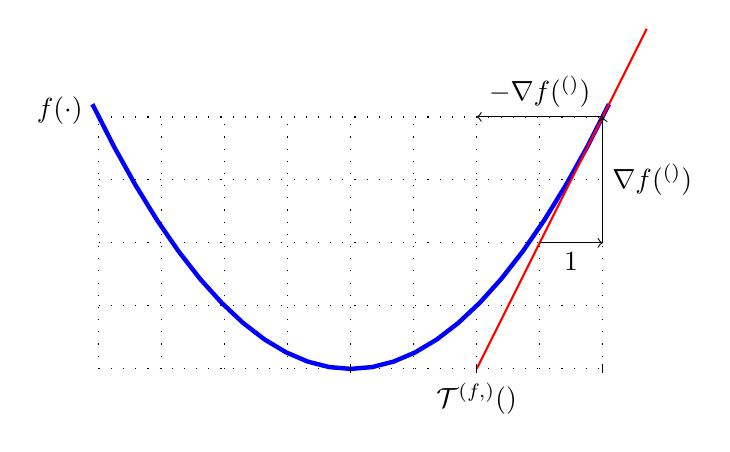
\begin{tikzpicture}[scale=0.8]
					\draw[loosely dotted] (-4,0) grid (4,4);
					\draw[blue, ultra thick, domain=-4.1:4.1] plot (\x,  {(1/4)*\x*\x});
					\draw[red, thick, domain=2:4.7] plot (\x,  {2*\x - 4});
					\draw[<-] (4,4) -- node[right] {$\nabla f(\weights^{(\itercntr)})$} (4,2);
					\draw[->] (4,4) -- node[above] {$-\lrate \nabla f(\weights^{(\itercntr)})$} (2,4);
					\draw[<-] (4,2) -- node[below] {$1$} (3,2) ;
					%\draw[->] (-4.25,0) -- (4.25,0) node[right] {$a$};
					\node[left] at (-4.1, 4.1) {$f(\cdot)$}; 
					\draw[shift={(0,0)}] (0pt,2pt) -- (0pt,-2pt) node[below] {$\overline{\weights}$};
					\draw[shift={(4,0)}] (0pt,2pt) -- (0pt,-2pt) node[below] {$\weights$};
					\draw[shift={(2,0)}] (0pt,2pt) -- (0pt,-2pt) node[below] {$\mathcal{T}^{(f,\lrate)}(\weights)$};
				\end{tikzpicture}
			\end{center}
			\caption{El paso básico de \gls{gradient} \eqref{equ_def_gd_basic_dict} mapea un vector $\weights$ 
			al vector actualizado $\weights'$. Define un operador 
			$\mathcal{T}^{(f,\lrate)}(\cdot): \mathbb{R}^{\nrfeatures} \rightarrow \mathbb{R}^{\nrfeatures}:
			 \weights \mapsto \widehat{\weights}$.}
			\label{fig_basic_GD_step_single_dict}
		\end{figure}
		Nótese que el paso de \gls{gradient} \eqref{equ_def_gd_basic_dict} optimiza localmente - 
		en una \gls{neighborhood} cuyo tamaño está determinado por el \gls{stepsize} $\lrate$ - una aproximación lineal 
		de la función $f(\cdot)$. Un  \gls{generalization} natural de \eqref{equ_def_gd_basic_dict} es optimizar localmente
		la función misma - en lugar de su aproximación lineal - de tal manera que:
		\begin{align} 
		\label{equ_approx_gd_step_dict}
		\widehat{\weights} = \argmin_{\weights' \in \mathbb{R}^{\dimlocalmodel}} f(\weights')\!+\!(1/\lrate)\normgeneric{\weights-\weights'}{2}^2. 
		\end{align}
		Intencionalmente usamos el mismo símbolo $\lrate$ para el parámetro en \eqref{equ_approx_gd_step_dict} 
		que en el \gls{stepsize} de \eqref{equ_def_gd_basic_dict}. Mientras mayor sea el valor de $\lrate$ en 
		\eqref{equ_approx_gd_step_dict}, más progreso hará la actualización en la reducción del valor de la función $f(\widehat{\weights})$. 
		Nótese que, al igual que el paso de \gls{gradient}  \eqref{equ_def_gd_basic_dict}, 
		la actualización \eqref{equ_approx_gd_step_dict} también define un operador (típicamente no lineal)  
		parametrizado por la función $f(\cdot)$ y el parámetro $\lrate$. Para una función \gls{convex}  
		$f(\cdot)$, este operador es conocido como el \gls{proxop} de $f(\cdot)$ \cite{ProximalMethods}. 
		},first={paso de gradiente},text={paso de gradiente}}
	

\newglossaryentry{proxop}{name={operador proximal},description={Dada una funcion\gls{convex}\index{operador proximal}   
		 $f(\weights')$, definimos su operador proximal como \cite{ProximalMethods,Bauschke:2017} 
		$$\proximityop{f(\cdot)}{\weights}{\rho}\defeq \argmin_{\weights' \in \mathbb{R}^{\dimlocalmodel}} \bigg[ f(\weights')\!+\!(\rho/2) \normgeneric{\weights- \weights'}{2}^{2}\bigg] \mbox{ with } \rho > 0. $$ 
		Como se ilustra en la Figura \ref{fig_proxoperator_opt_dict}, evaluar el operador proximal 
		equivale a minimizar una variante penalizada de $f(\weights')$. El término de penalización es 
		la distancia euclidiana cuadrada escalada hacia un vector dado $\weights$ (que es la entrada del operador proximal). 
		%\Gls{convex} functions for which the proximal operator can be computed efficiently 
		%is sometimes referred to as \emph{proximable} or \emph{simple} \cite{Condat2013}. 
		El operador proximal puede interpretarse como una \gls{generalization} del \gls{gradstep}, definido 
		para una función \gls{smooth} y \gls{convex} $f(\weights')$. De hecho, realizar un 
		\gls{gradstep} con \gls{stepsize} $\lrate$ en el vector actual $\weights$ 
		es lo mismo que aplicar el \gls{proxop}de la función $\tilde{f}(\weights')= \big( \nabla f(\weights)\big)^{T} (\weights'-\weights)$ 
		y usar $\rho=1/\lrate$.
			\begin{figure}[H]
			\begin{center}
				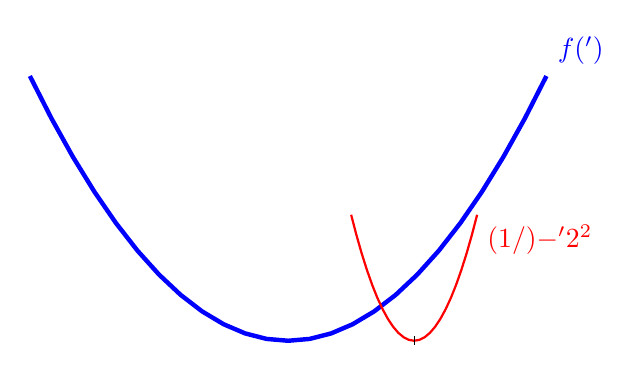
\begin{tikzpicture}[scale=0.8]
					% Original quadratic function
					\draw[blue, ultra thick, domain=-4.1:4.1] plot (\x, {(1/4)*\x*\x}) node[above right] {$f(\weights')$};		
					% Quadratic function with larger curvature, centered at w = 2
					\draw[red, thick, domain=1:3] plot (\x, {2*(\x - 2)*(\x - 2)}) node[below right] {$(1/\lrate)\normgeneric{\weights-\weights'}{2}^{2}$};
					% Axes
					% Minimum point of second curve
					\draw[shift={(2,0)}] (0pt,2pt) -- (0pt,-2pt) node[below] {$\weights$};
					%\node at (2,0.5) [anchor=north] {$\weights$};
				\end{tikzpicture}
			\end{center}
			\caption{Un \gls{gradstep} generalizado actualiza un vector $\weights$ minimizando una versión penalizada 
				de la función $f(\cdot)$. El término de penalización es la distancia euclidiana cuadrada escalada entre 
				la variable de optimización $\weights'$ y el vector dado $\weights$.\label{fig_proxoperator_opt_dict}}
		\end{figure}
		},first={operador proximal},text={operador proximal}}

\newglossaryentry{proximable}{name={proximable},description={Una funcion \index{proximable} 
		\gls{convex} para la cual el \gls{proxop} puede calcularse de manera eficiente 
		se denomina a veces proximable o simple \cite{Condat2013}.},
		first={proximable},text={proximable}
		
		}


\newglossaryentry{connected}
		{name={grafo conexo},
			description={
				Un \gls{graph} no dirigido\index{grafo conexo} $\graph=\pair{\nodes}{\edges}$ es conexo si todo subconjunto no vacío $\nodes' \subset \nodes$
				tiene al menos una arista que lo conecta con $\nodes \setminus \nodes'$.
			},
			first={grafo conexo},text={grafo conexo}
		}
	
	

\newglossaryentry{mvndist}{name ={distribución normal multivariante},description=
{
	La distribución normal multivariante\index{distribución normal multivariante} $\mvnormal{\vm}{\mC}$ es una
	familia importante de \gls{probdist}s para una \gls{rv} continua $\featurevec \in \mathbb{R}^{\nrfeatures}$ \cite{BertsekasProb,GrayProbBook,Lapidoth09}.
	Esta familia está parametrizada por la \gls{mean} $\vm$ y la \gls{covmtx} $\mC$ de $\featurevec$.
	Si la \gls{covmtx} es invertible, la \gls{probdist} de $\featurevec$ es
	$$p(\featurevec) \propto \exp\bigg(-(1/2) \big( \featurevec - \vm \big)^{T} \mC^{-1} \big( \featurevec - \vm \big) \bigg).$$
},
first={distribución normal multivariante},text={distribución normal multivariante}
}

\newglossaryentry{statasp}{name ={aspectos estadísticos}, description={Por aspectos estadísticos\index{aspectos estadísticos} 
		de un método de \gls{ml},  nos referimos a las propiedades de la \gls{probdist} de su salida bajo 
		un \gls{probmodel} para los \gls{data} introducidos en el método.},first={aspectos estadísticos},text={aspectos estadísticos}}

\newglossaryentry{compasp}{name ={aspectos computacionales}, description={Por aspectos 
		computacionales\index{aspectos computacionales} de un método de \gls{ml}, nos referimos principalmente a los recursos 
		computacionales requeridos para su implementación.
		Por ejemplo, si un método de \gls{ml} utiliza técnicas 
		de optimización iterativas para resolver \gls{erm}, sus aspectos computacionales incluyen: 1) cuántas 
		many operaciones aritméticas se necesitan para implementar una sola iteración(\gls{gradstep}); 
		y 2) cuántas iteraciones se requieren para obtener \gls{modelparams} útiles. Un ejemplo 
		importante de técnica de optimización iterativa es el  \gls{gd}.}, first={aspectos computacionales},text={aspectos computacionales}}

\newglossaryentry{zerooneloss}{name={$\bf 0/1$ loss},
	description={La \gls{loss} $0/1$ \index{$0/1$ loss} $\lossfunczo{\pair{\featurevec}{\truelabel}}{\hypothesis}$ 
		mide la calidad de un \gls{classifier} $\hypothesis(\featurevec)$ que genera una 
		\gls{prediction} $\predictedlabel$ (por ejemplo, mediante un umbral como en \eqref{equ_def_threshold_bin_classifier_dict}) 
		para la \gls{label} $\truelabel$ de un \gls{datapoint} con \gls{feature}s $\featurevec$. Es igual a $0$ si 
		la \gls{prediction} es correcta, es decir, 
	$\lossfunczo{\pair{\featurevec}{\truelabel}}{\hypothesis}=0$ cuando $\predictedlabel=\truelabel$. Es igual 
	a $1$ si la \gls{prediction} es incorrecta, es decir, $\lossfunczo{\pair{\featurevec}{\truelabel}}{\hypothesis}=1$ 
	cuando $\predictedlabel\neq\truelabel$.},
	sort=zerooneloss, 
    first={$0/1$ loss},text={$0/1$ loss}}

\newglossaryentry{probability}{name={probabilidad},
	description={Asignamos \index{probabilidad} un valor de probabilidad, típicamente elegido en el 
		intervalo $[0,1]$, a cada evento que pueda ocurrir en un experimento aleatorio \cite{KallenbergBook,BertsekasProb,BillingsleyProbMeasure,HalmosMeasure}.},
		first={probabilidad},text={probabilidad}}
	
\newglossaryentry{underfitting}{name={subajuste},
	description={Consideremos\index{subajuste} un método de \gls{ml} que utiliza \gls{erm} para aprender una \gls{hypothesis}
	con el \gls{minimum} \gls{emprisk} en un \gls{trainset} dado.
	Dicho método presenta subajuste del \gls{trainset} si no es capaz de aprender una \gls{hypothesis}
	con un \gls{emprisk} suficientemente pequeño sobre el \gls{trainset}.
	Si un método sufre de subajuste, típicamente tampoco podrá aprender una \gls{hypothesis}
	con un \gls{risk} pequeño.},
	first={subajuste},text={subajuste}
		}

\newglossaryentry{overfitting}{name={sobreajuste},description={Consideremos\index{overfitting} un 
		método de \gls{ml} que utiliza \gls{erm} para aprender una \gls{hypothesis} con el \gls{minimum} \gls{emprisk} en 
		un \gls{trainset} dado. Dicho método presenta sobreajuste del \gls{trainset} si aprende 
		una \gls{hypothesis} con un \gls{emprisk} pequeño sobre el \gls{trainset} pero una \gls{loss} significativamente mayor fuera de él \gls{trainset}.},first={sobreajuste},text={sobreajuste}}

\newglossaryentry{gdpr}{name={reglamento general de protección de datos (RGPD)},description={
			El\index{reglamento general de protección de datos (RGPD)} RGPD
			fue promulgado por la Union Europea (EU), y entró en efecto el 25 de Mayo de 2018 \cite{GDPR2016}. 
			Protege la privacidad y los derechos sobre los \gls{data} de los individuos dentro de la EU. 
			El RGPD tiene implicaciones significativas sobre cómo se recopilan, almacenan y utilizan los \gls{data} en aplicaciones de \gls{ml}.
			Las disposiciones clave incluyen:
			\begin{itemize}
				\item \Gls{dataminprinc}: los sistemas de \gls{ml} deben utilizar únicamente la cantidad necesaria de  
				\gls{data} personal para su propósito.
				\item \Gls{transparency} y \gls{explainability}: los sistemas de \gls{ml} deben permitir a sus usuarios comprender 
				cómo se toman las decisiones que los afectan.
				\item Derechos del titular de los datos \Gls{data}:los usuarios deben tener la posibilidad de acceder, rectificar y eliminar sus \gls{data}, así como oponerse a decisiones automatizadas y perfiles.
				\item Responsabilidad: las organizaciones deben garantizar una seguridad robusta de los \gls{data} y demostrar 
				cumplimiento mediante documentación y auditorías periódicas.
			\end{itemize}
			}, 
	first={reglamento general de protección de datos (RGPD)},text={RGPD}}
	
\newglossaryentry{gaussrv}{name={variable aleatoria gaussiana (VA gaussiana)},description={
		Una \index{variable aleatoria gaussiana (VA gaussiana)} \gls{rv} gaussiana estándar es una \gls{rv} 
		real $x$ con \gls{pdf} \cite{papoulis,BertsekasProb,GrayProbBook}
		\begin{equation}
			\nonumber
			p(x) = \frac{1}{\sqrt{2\pi}} \exp^{-x^2/2}. 
		\end{equation}
		Dada una \gls{rv} gaussiana estándar $x$, podemos construir una \gls{rv} gaussiana general $x'$ con 
		\gls{mean} $\mu$ y \gls{variance} $\sigma^2$ mediante $x' \defeq \sigma (x+\mu)$. La \gls{probdist} de una 
		\gls{rv} gaussiana se conoce como distribución normal, denotada $\mathcal{N}(\mu,\sigma)$.  \\ 
		Un vector aleatorio gaussiano $\featurevec \in \mathbb{R}^{\featuredim}$ con 
		\gls{covmtx} $\mathbf{C}$ y \gls{mean} ${\bm \mu}$ puede construirse como 
		$\featurevec \defeq \mathbf{A} \big( \vz + {\bm \mu} \big)$. Aquí, $\mA$ 
		es cualquier matriz que satisface $\mA\mA^{T} = \mC$ y $\vz \defeq \big( z_{1},\ldots,z_{\featuredim} \big)^{T}$
		es un vector cuyos elementos son \gls{iid} gaussianas estándar \gls{rv}s $z_{1},\ldots,z_{\featuredim}$. Los procesos aleatorios gaussianos generalizan
		los vectores aleatorios gaussianos aplicando transformaciones lineales a 
		a secuencias infinitas de \gls{rv}s gaussianas estándar \cite{Rasmussen2006Gaussian}.\\
		Las \gls{rv}s gaussianas se utilizan ampliamente como \gls{probmodel}s en el análisis estadístico de métodos de \gls{ml}.
		Su importancia se debe, en parte, al teorema del límite central, que establece que el promedio de un número creciente de \gls{rv}s independientes
		(aunque no sean gaussianas) converge a una \gls{rv} gaussiana \cite{ross2013first}. 
},first={variable aleatoria gaussiana (VA gaussiana)},text={VA gaussiana}

\newglossaryentry{trustAI}{name={inteligencia artificial confiable (IA confiable)},description=
		{Además de los \gls{compasp} y los \gls{statasp}, un tercer aspecto principal 
		en el diseño de métodos de \gls{ml} es su confiabilidad\index{inteligencia artificial confiable (IA confiable)} \cite{pfau2024engineeringtrustworthyaideveloper}. 
		La Unión Europea ha propuesto siete requisitos clave (KRs) para una \gls{ai} confiable 
		(que típicamente se basa en métodos de \gls{ml}) \cite{ALTAIEU}: 
	\begin{enumerate}[label=\arabic*)]
		\item KR1 - Agencia y supervisión humana;
		\item KR2 - Robustez técnica y seguridad;
		\item KR3 - Privacidad y gobernanza de los \gls{data};
		\item KR4 - Transparencia;
		\item KR5 - Diversidad, no discriminación y equidad; 
		\item KR6 - Bienestar social y ambiental;
		\item KR7 - Responsabilidad. 
	\end{enumerate}
	},first={inteligencia artificial confiable (IA confiable)},text={trustworthy AI}}

\newglossaryentry{sqerrloss}{name={pérdida de error cuadrático},description={La \gls{loss} de
		error cuadrático\index{pérdida de error cuadrático} mide el error de \gls{prediction} de una 
		\gls{hypothesis} $\hypothesis$ al predecir una \gls{label} numérica $\truelabel \in \mathbb{R}$ 
		a partir de las \gls{feature}s $\featurevec$ de un \gls{datapoint}. Se define 
	como 
\begin{equation} 
	\nonumber
%	\label{equ_squared_loss_gls}
	\lossfunc{(\featurevec,\truelabel)}{\hypothesis} \defeq \big(\truelabel - \underbrace{\hypothesis(\featurevec)}_{=\predictedlabel} \big)^{2}. 
\end{equation} 
},first={pérdida de error cuadrático},text={pérdida de error cuadrático}}


 \newglossaryentry{projection}{name={proyección}, 
       description={Consideremos\index{proyección} un subconjunto $\paramspace \subseteq \mathbb{R}^{\dimlocalmodel}$ del 
	   \gls{euclidspace} de dimensión $\dimlocalmodel$. Definimos la proyección $\projection{\paramspace}{\weights}$
	   de un vector $\weights \in \mathbb{R}^{\dimlocalmodel}$ sobre $\paramspace$ como
		\begin{equation} 
   	    \label{equ_def_proj_generic_dict}
  	     \projection{\paramspace}{\weights} = \argmin_{\weights' \in \paramspace} \normgeneric{\weights - \weights'}{2}. 
         \end{equation}
		 En otras palabras, $\projection{\paramspace}{\weights}$ es el vector en $\paramspace$ más cercano a $\weights$. 
		 La proyección está bien definida solo para aquellos subconjuntos $\paramspace$ para los cuales existe el \gls{minimum} anterior \cite{BoydConvexBook}.},
		 first={proyección},text={proyección}}


\newglossaryentry{projgd}{name={descenso por gradiente proyectado (GD proyectado)},
description={Consideremos un método basado en \gls{erm} que utiliza un \gls{model} parametrizado con  
un \gls{paramspace} $\paramspace \subseteq \mathbb{R}^{\dimlocalmodel}$. Aun si la
\gls{objfunc} de \gls{erm} es \gls{smooth}, no podemos usar el \gls{gd} básico, ya 
ya que este no toma en cuenta las restricciones sobre la variable de optimización (es decir, los \gls{modelparams}). 
El \gls{gd} proyectado\index{descenso por gradiente proyectado (GD proyectado)} 
extiende el \gls{gd} básico para controlar restricciones sobre la variable de optimización(es decir, los \gls{modelparams}). 
Una sola iteración del \gls{gd} proyectado consiste primero en realizar un \gls{gradstep} 
y luego proyectar el resultado sobre el \gls{paramspace}.
\begin{figure}[H]
	\begin{center}
		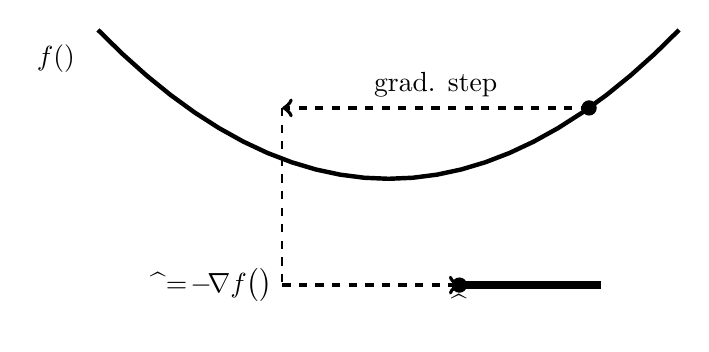
\begin{tikzpicture}[scale=0.9]
			\node [right] at (-5.1,1.7) {$f(\weights)$} ;
			\draw[ultra thick, domain=-4.1:4.1] plot (\x,  {(1/8)*\x*\x});
		%	\draw[dashed, thick, domain=1:3.6] plot (\x,  {\x - 1}) node[right] {$ f\big(\weights^{(\itercntr)}\big)\!+\!\big(\weights\!-\!\weights^{(\itercntr)}\big)^{T} \nabla f\big(\weights^{(\itercntr)}\big)$};
			\draw [fill] (2.83,1) circle [radius=0.1] node[right] {$\weights$};
			\draw[line width =0.5mm,dashed,->] (2.83,1) -- node[midway,above] {grad. step} (-1.5,1);
			\draw[line width =0.2mm,dashed] (-1.5,1) --(-1.5,-1.5)  node [below, left]{$\widehat{\weights}=\weights\!-\!\lrate \nabla f\big(\weights\big)$} ;
			\draw[line width =0.5mm,dashed,->] (-1.5,-1.5)  -- node[midway,above] {} (1,-1.5) ; 
			\draw [fill] (1,-1.5) circle [radius=0.1] node[below] {$\projection{\paramspace}{\widehat{\weights}}$};
			\draw[line width=1mm] (1,-1.5) -- (3,-1.5) node[midway, above] {$\paramspace$};
		\end{tikzpicture}
		\vspace*{-5mm}
	\end{center}
	\caption{\gls{gd} proyectado amplía un \gls{gradstep} básico con una \gls{projection} de regreso 
	al conjunto de restricciones $\paramspace$.}
	\label{fig_projected_GD_dict}
\end{figure}},first={descenso por gradiente proyectado (GD proyectado)},text={GD proyectado}}

\newglossaryentry{diffpriv}
{name=privacidad diferencial (DP),
  description={
  	Consideremos\index{differential privacy (DP)} un método de \gls{ml} $\algomap$ que recibe como entrada un \gls{dataset} (por ejemplo, el \gls{trainset} 
  	usado para \gls{erm}) y entrega una salida $\algomap(\dataset)$. La salida 
  	puede ser los \gls{modelparams} aprendidos o las \gls{prediction}es para ciertos \gls{datapoint}s. 
  	DP es una medida precisa de la \gls{privleakage} ocasionada al revelar dicha salida.
	Aproximadamente, un método de \gls{ml} es diferencialmente privado si la \gls{probdist} 
  	de la salida $\algomap(\dataset)$ no cambia significativamente cuando se modifica el \gls{sensattr} 
  	de un solo \gls{datapoint} del \gls{trainset}. Nótese que la DP 
  	se basa en un \gls{probmodel} para un método de \gls{ml}, es decir, interpretamos su salida $\algomap(\dataset)$ 
  	como la \gls{realization} de un \gls{rv}. La aleatoriedad en la salida puede asegurarse añadiendo intencionalmente la
  	\gls{realization} de una \gls{rv} auxiliar (ruido) a la salida del método de  \gls{ml}.
	}, 
	first = {privacidad diferencial (DP)}, text={DP} 
}

\newglossaryentry{privprot}
{name=protección de la privacidad,
     description={Consideremos\index{protección de la privacidad} un método de \gls{ml}  $\algomap$ que recibe como entrada 
	 una \gls{dataset} $\dataset$ y entega una salida $\algomap(\dataset)$. La salida 
	 puede ser los \gls{modelparams} aprendidos $\widehat{\weights}$ o una \gls{prediction} 
	 $\learnthypothesis(\featurevec)$ obtenida para un \gls{datapoint} específico con \gls{feature}s 
	 $\featurevec$. Muchas aplicaciones importantes de \gls{ml} involucran \gls{datapoint}s 
		que representan a personas. Cada \gls{datapoint} se caracteriza por \gls{feature}s $\featurevec$, 
		posiblemente una \gls{label} $\truelabel$, y un \gls{sensattr} $\sensattr$ (por ejemplo, un diagnóstico medico). 
		Mas o menos, la protección de la privacidad significa que debería ser imposible inferir, de la salida $\algomap(\dataset)$, 
		cualquier \gls{sensattr}s de los \gls{datapoint}s en $\dataset$. Matemáticamente, la protección de privacidad requiere que  
		el mapeo $\algomap(\dataset)$ no sea invertible. En general, el solo hacer que  $\algomap(\dataset)$ no sea invertible 
		no es suficiente. Necesitamos que sea suficientemente no invertible. 
	}, 
	first = {protección de la privacidad}, text={protección de la privacidad} 
}

\newglossaryentry{privleakage}
{
	name=filtración de privacidad,
	description={Consideremos\index{privacy leakage} una aplicacion de \gls{ml} que procesa un
	\gls{dataset} $\dataset$ y produce una salida, como las \gls{prediction}es 
	obtenidas para nuevos \gls{datapoint}s. Se produce una filtración de privacidad 
	cuando la salida contiene información privada sobre un \gls{feature} de un 
	\gls{datapoint} (que podría representar a una persona) en $\dataset$. Basado en la \gls{probmodel} 
	para la generacion de los \gls{data}, podemos medir la filtración de privacidad usando la \gls{mutualinformation} 
	entre la salida y la \gls{feature} sensible. Otra medida cuantitativa de la filtración de privacidad 
	es la \gls{diffpriv}. Las relaciones entre las diferentes medidas de filtración de privacidad han sido estudiadas en la literatura (véa \cite{InfThDiffPriv}). 
	}, 
	first = {filtración de privacidad}, text={filtración de privacidad} 
}



\newglossaryentry{probmodel}
{
	name=modelo probabilístico,
	description={Un \gls{model} probabilístico\index{modelo probabilístico} interpreta los \gls{datapoint}s 
		como \gls{realization}es de \gls{rv}s con una \gls{probdist} conjunta. Esta \gls{probdist} conjunta típicamente 
		incluye \gls{parameters} que deben seleccionarse manualmente or o aprenderse usando métodos de inferencia estadística  
		como la estimación por \gls{maxlikelihood} \cite{LC}. }, 
	first = {modelo probabilístico}, text={modelo probabilístico} 
}



\newglossaryentry{mean}
{
	name=media,
	description={La\index{media} \gls{expectation} $\expect \{ \featurevec \}$ de una \gls{rv} numérica $\featurevec$.}, 
		first = {media}, text={media} 
}

\newglossaryentry{variance}
{
	name={varianza},
	description={La\index{varianza} varianza de una \gls{rv} real $\feature$ se define como la \gls{expectation} 
		$\expect\big\{ \big( x - \expect\{x \} \big)^{2} \big\}$ de la diferencia cuadrada entre $\feature$ 
		y su \gls{expectation} $\expect\{x \}$. Extendemos esta definición a \gls{rv}s vectoriales$\featurevec$ 
		como $\expect\big\{ \big\| \featurevec - \expect\{\featurevec \} \big\|_{2}^{2} \big\}$.} ,
		first={varianza},text={varianza} 
}

\newglossaryentry{nn}
{
	name={vecino más cercano (NN)},
	description={Los métodos de vecino más cerano (NN)\index{vecino más cercano (NN)} aprenden una \gls{hypothesis} 
		$\hypothesis: \featurespace \rightarrow \labelspace$ cuyo valor $\hypothesis(\featurevec)$ 
		se determina únicamente por los \gls{neighbors} más cercanos dentro de un \gls{dataset}. Distintos 
		métodos usan diferentes medidas para determinar los \gls{neighbors} más cercanos. Si los \gls{datapoint}s 
		se caracterizan por \gls{featurevec}s numéricos, podemos usar la distancia euclidiana como medida.  
		the metric.},
	first={vecino más cercano (NN)},text={NN} 
}

\newglossaryentry{neighborhood}
{
	name={entorno},
	description={El\index{entorno} entorno de un nodo $\nodeidx \in \nodes$ es 
	el subconjunto de nodos constituido por los \gls{neighbors} de $\nodeidx$.},
	first={entorno},text={entorno} 
}


\newglossaryentry{neighbors}
{
	name={vecinos},
	description={Los\index{vecinos} vecinos de un nodo $\nodeidx \in \nodes$ 
	dentro de un \gls{empgraph} son los nodos $\nodeidx' \in \nodes \setminus \{ \nodeidx\}$ conectados con $\nodeidx$ por una arista.},
	first={vecinos},text={vecinos} 
}

\newglossaryentry{bias}
{
	name={sesgo},
	description={Consideremos\index{sesgo} un método de \gls{ml} que utiliza un \gls{hypospace} $\hypospace$ parametrizado. 
		Este aprende los \gls{modelparams} $\weights \in \mathbb{R}^{\dimlocalmodel}$ utilizando el \gls{dataset} $$ \dataset=\big\{ \pair{\featurevec^{(\sampleidx)}}{\truelabel^{(\sampleidx)}} \big\}_{\sampleidx=1}^{\samplesize}.$$ 
		Para analizar las propiedades del método de \gls{ml}, típicamente interpretamos los \gls{datapoint}s como \gls{realization}es 
		de \gls{iid} \gls{rv}s, $$ \truelabel^{(\sampleidx)} = \hypothesis^{(\overline{\weights})}\big( \featurevec^{(\sampleidx)} \big) + \bm{\varepsilon}^{(\sampleidx)}, \sampleidx=1,\ldots,\samplesize.$$ 
		Entonces podemos interpetar el método de \gls{ml} como un estimador $\widehat{\weights}$ 
		calculado a partir de $\dataset$ (por ejemplo, resolviendo \gls{erm}). El sesgo (cuadrado) del estimador $\widehat{\weights}$ 
		se define como $\biasterm^{2} \defeq \big\| \expect \{ \widehat{\weights}  \}- \overline{\weights}\big\|_{2}^{2}$. },
		first={sesgo},text={sesgo} 
}

\newglossaryentry{classification}
{name={clasificación},
 description={La clasificación\index{classification} es la tarea de determinar una
 	etiqueta $\truelabel$  con valor discreto para un \gls{datapoint}, basado únicamente en sus 
	 \gls(feature)s $\featurevec$. La etiqueta $\truelabel$ pertenece a un conjunto finito, como por ejemplo 
 	$\truelabel \in \{-1,1\}$ o $\truelabel \in \{1,\ldots,19\}$, y representa la 
 	categoría a la que pertenece el \gls{datapoint}.},
	first={clasificación},text={clasificación} 
}


% a bit awkward, come back to this. 
\newglossaryentry{privfunnel}
{name={embudo de privacidad},
 description={El\index{privacy funnel} embudo de privacidad es un método para aprender \gls{feature}s 
	amigables con la privacidad de los \gls{datapoint}s \cite{PrivacyFunnel}.},
 first={embudo de privacidad},text={embudo de privacidad} 
}




\newglossaryentry{condnr}
{
	name={número de condición},
	description={El número de condición\index{número de condición} $\kappa(\mathbf{Q}) \geq 1$ de una 
		matriz definida positiva $\mathbf{Q} \in \mathbb{R}^{\featurelen \times \featurelen}$ es el cociente 
		$\alpha /\beta  $ entre el 
		mayor $\alpha$ y el menor $\beta$ \gls{eigenvalue} de 
		$\mathbf{Q}$. El número de condición es útil para el análisis de métodos de \gls{ml}. 
		La complejidad computacional de los \gls{gdmethods} para \gls{linreg} depende críticamente del número 
		de condición de la matriz $\mQ = \mX \mX^{T}$, donde $\mX$  es la \gls{featuremtx}  
		del \gls{trainset}. Es por eso que desde una perspectiva computacional, preferimos \gls{feature}s de los 
		\gls{datapoint}s que hagan que $\mQ$ tenga un número de condición cercano a $1$.},first={número de condición},text={número de condición} 
}

\newglossaryentry{classifier}
{
	name={clasificador},
	description={Un clasificador\index{clasificador} es una \gls{hypothesis} (función) $\hypothesis(\featurevec)$ 
		usada para predecir una \gls{label} que toma valores de un \gls{labelspace} finito. Podemos usar directamente 
		el valor $\hypothesis(\featurevec)$ como \gls{prediction} $\predictedlabel$ para 
		la \gls{label}. pero normalmente se usa una función $\hypothesis(\cdot)$ que entrega 
		una cantidad numérica. La \gls{prediction} es obtenida a travez de un paso de umbral. 
		Por ejemplo, en un problema de \gls{classification} binaria con \label{labelspace} $\labelspace \in  \{ -1,1\}$, 
		podríamos usar una \gls{hypothesis} de valores reales $\hypothesis(\featurevec) \in \mathbb{R}$ 
		como clasificador. Una \gls{prediction} $\predictedlabel$ puede obtenerse mediante:  
		 \begin{equation} 
		 	\label{equ_def_threshold_bin_classifier_dict}
		 	\predictedlabel =1   \mbox{ for } \hypothesis(\featurevec)\!\geq\!0 \mbox{ and } 	\predictedlabel =-1  \mbox{ otherwise.}
	 		\end{equation}
 		Podemos caracterizar un clasificador mediante sus \gls{decisionregion}es $\decreg{a}$, para 
 		cada valor posible de \gls{label} $a \in \labelspace$. },first={clasificador},text={clasificador} 
}

\newglossaryentry{emprisk}
{name={riesgo empírico},
  description={El \gls{risk} empírico\index{riesgo empírico} $\emprisk{\hypothesis}{\dataset}$ 
  	de una \gls{hypothesis} sobre un \gls{dataset} $\dataset$ es la \gls{loss} promedio incurrida 
  	por $\hypothesis$ al aplicarse a los \gls{datapoint}s en el $\dataset$.},
  first={riesgo empírico},text={riesgo empírico} 
}

% is it not the number of edges connected to the node instead of the neigbors?  could be the same thing, just wondering about the actual definition here. 
\newglossaryentry{nodedegree}
{name={grado de nodo},
	description={El grado\index{grado de nodo} $\nodedegree{\nodeidx}$ de un nodo $\nodeidx \in \nodes$ 
		en un \gls{graph} no dirigido, es el número de sus \gls{neighbors}, es decir, $\nodedegree{\nodeidx} \defeq \big|\neighbourhood{\nodeidx}\big|$.},
		first={grado de nodo},text={grado de nodo} 
}

\newglossaryentry{graph}
{name={grafo},
	description={Un grafo\index{graph} $\graph = \pair{\nodes}{\edges}$ es un par compuesto por un  
		conjunto de nodos $\nodes$ y un conjunto de aristas $\edges$. En su forma màs general, un grafo se 
		específica por una función que asigna a cada arista $\edgeidx \in \edges$ un par de nodos \cite{RockNetworks}. 
		Un grupo importante de grafos son los grafos no dirigidos. Un grafo simple no dirigido  
		es obtenida identificando cada arista $\edgeidx \in \edges$ con dos nodos diferentes $\{\nodeidx,\nodeidx'\}$. 
		Los grafos etiquetados asignan un peso númerico especifico \gls{weights} $\edgeweight_{\edgeidx}$ a cada 
		arista $\edgeidx \in \edges$.},first={graph},text={graph} 
}

% i think UCB might be a unfinished definition. Check with Alex on this one. 

\newglossaryentry{ucb}
{name={límite superior de confianza (UCB)},
	description={Consideremos\index{límite superior de confianza (UCB)} una aplicacion de \gls{ml} 
		 que predice, en cada nueva iteración,
		 la acción óptima dentro de un conjunto finito de acciones posibles. Medimos la utilidad  
		 de una predicción \gls{prediction} (al tomar una accion específica) por un \gls{reward} númerico. 
		 Un \gls{probmodel} popular utilizado para este tipo de problema de decisiones secuenciales
		 es el problema multibrazo(multi-armed bandit) $\ldots$. 
		 
		 El premio obtenido por cada acción puede modelarse como una \gls{realization} de una\gls{rv} 
		 con cierta \gls{mean} y \gls{variance}.},first={límite superior de confianza (UCB)},text={UCB} 
}


\newglossaryentry{optimism in the face of uncertainty}
{name={optimismo ante la incertidumbre},
	description={Los metodos de \gls{ml}\index{optimismo ante la incertidumbre} aprenden \gls{modelparams} $\weights$ 
		de acuerdo con algún criterio de desempeño $\bar{f}(\weights)$. Sin embargo, normalmente 
		no pueden acceder directamente a $\bar{f}(\weights)$  pero dependen de una estimación (o aproximación) de $f(\weights)$. 
		Por ejemplo, los métodos basados en \gls{erm} usan la \gls{loss} promedio en un \gls{dataset} (por ejemplo, el \gls{trainset}) 
		como estimación del \gls{risk} de una \gls{hypothesis}. Usando un \gls{probmodel}, se puede construir 
		un intervalo  de confianza. 
	$\big[ l^{(\weights)},  u^{(\weights)} \big]$ para cada elección $\weights$ de los \gls{modelparams}.
	Una construcción simple es $l^{(\weights)} \defeq f(\weights) - \sigma/2$, $u^{(\weights)} \defeq f(\weights)+ \sigma/2$, 
	donde $\sigma$ representa una medida de la desviación entre $f(\weights)$ y $\bar{f}(\weights)$. 
	También se pueden usar otras construcciones del intervalo, mientras se aseguren que $\bar{f}(\weights) \in\big[ l^{(\weights)},  u^{(\weights)} \big]$ 
	con un probabilidad suficientemente alta. Siendo optimistas, elegimos los \gls{modelparams} 
	según el valor más favorable - pero realista - del criterio de desempeño $\tilde{f}(\weights) \defeq  l^{(\weights)}$. 
	Dos ejemplos de métodos de \gls{ml} que usan una construcción optimista de una \gls{objfunc} 
	son métodos de \gls{srm} \cite[Ch. 11]{ShalevMLBook} y \gls{ucb}  para decisiones secuenciales \cite[Sec. 2.2]{Bubeck2012}. 
		\begin{figure}[H]
				\begin{center}
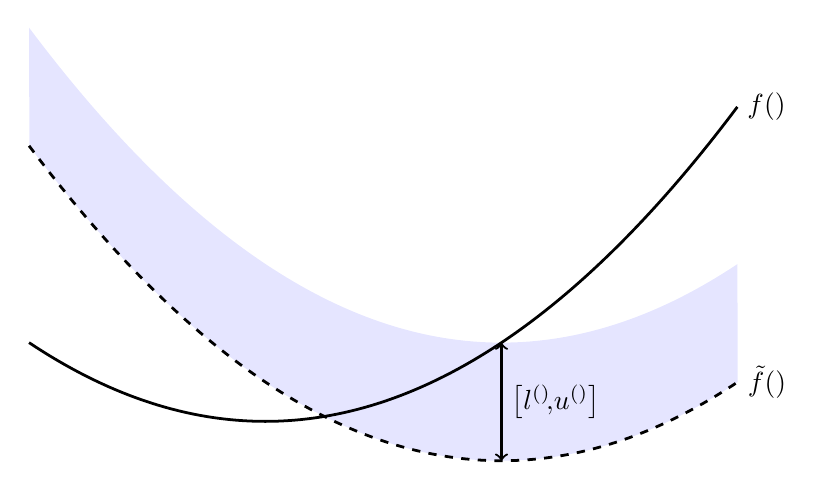
\begin{tikzpicture}[x=3cm, y=1cm]
  % Filled band around the quadratic curve with different boundary curves
\fill[blue!10] 
(-1, 5) -- plot[domain=-2:1, samples=100] ({\x+1}, {\x*\x + 1}) -- 
plot[domain=1:-2, samples=100] ({\x+1}, {\x*\x - 0.5}) -- cycle;
  \node[anchor=west] at (2, 4) {$f(\weights)$};
  \draw[line width=1, domain=-2:1, samples=100,dashed] plot  ({\x+1}, {\x*\x -0.5}) node[right] {$\tilde{f}(\weights)$};
   \draw[line width=1, domain=-1:2, samples=100] plot ({\x}, {\x*\x});
  \draw[<->, thick] (1, -0.5) -- (1, 1) node[midway, right] {$\big[ l^{(\weights)}\!,\!u^{(\weights)} \big]$};
\end{tikzpicture}
\caption{Los métodos de \gls{ml} aprenden \gls{modelparams} $\weights$ usando una estimación de $f(\weights)$ como 
	aproximación del criterio de desempeño $\bar{f}(\weights)$. Usando un \gls{probmodel}, se pueden construir intervalos de confianza $\big[ l^{(\weights)},  u^{(\weights)} \big]$ 
	que contienen $\bar{f}(\weights)$ con alta probabilidad. La mejor medida plausible del desempeño para una elección especifica $\weights$ es $\tilde{f}(\weights) \defeq l^{(\weights)}$.} 
	\end{center}
		\end{figure}},first={optimismo ante la incertidumbre},text={optimismo ante la incertidumbre} 
}

\newglossaryentry{empgraph}
{name={federated learning network (FL network)},
	description={A federated network\index{federated learning network (FL network)} is an undirected weighted \gls{graph} whose 
		nodes represent \gls{data} generators that aim to train a local (or personalized) \gls{model}. 
		Each node in a federated network represents some \gls{device} capable of collecting a \gls{localdataset} 
		and, in turn, train a \gls{localmodel}. 
	    \Gls{fl} methods learn a local \gls{hypothesis} $\localhypothesis{\nodeidx}$, for 
	    each node $\nodeidx \in \nodes$, such that it incurs small \gls{loss} on the \gls{localdataset}s.},first={federated learning network (FL network)},text={FL network} 
}

\newglossaryentry{norm}
{name={norm},
	description={A norm\index{norm} is a function that maps each (vector) element 
		of a linear vector space to a non-negative real number. This function must be homogeneous and definite, and it must satisfy the triangle inequality \cite{HornMatAnalysis}. },
	first={norm},text={norm} 
}

\newglossaryentry{explanation}
{name={explanation},
	description={One approach to make \gls{ml} methods transparent is to provide an 
		explanation\index{explanation} along with the \gls{prediction} delivered by an 
		\gls{ml} method. Explanations can take on many different forms. An explanation 
		could be some natural text or some quantitative measure for the importance 
		of individual \gls{feature}s of a \gls{datapoint} \cite{Molnar2019}. We can also 
		use visual forms of explanations, such as intensity plots for image \gls{classification} \cite{GradCamPaper}.},
	first={explanation},text={explanation} 
}

\newglossaryentry{risk}
{name={risk},
	description={Consider\index{risk} a \gls{hypothesis} $\hypothesis$ used to predict the \gls{label} 
		$\truelabel$ of a \gls{datapoint} based on its \gls{feature}s $\featurevec$. We measure 
		the quality of a particular \gls{prediction} using a \gls{lossfunc} $\lossfunc{(\featurevec,\truelabel)}{\hypothesis}$. 
		If we interpret \gls{datapoint}s as the \gls{realization}s of \gls{iid} \gls{rv}s, 
		also the $\lossfunc{(\featurevec,\truelabel)}{\hypothesis}$ becomes the \gls{realization} 
		of an \gls{rv}. The \gls{iidasspt} allows us to define the risk of a \gls{hypothesis} 
		as the expected \gls{loss} $\expect \big\{\lossfunc{(\featurevec,\truelabel)}{\hypothesis} \big\}$. 
		Note that the risk of $\hypothesis$ depends on both the specific choice for the \gls{lossfunc} and the 
		\gls{probdist} of the \gls{datapoint}s.},
	first={risk},text={risk} 
}

\newglossaryentry{actfun}
{name={activation function},
	description={Each\index{activation function} artificial neuron within an \gls{ann} is 
		assigned an activation function $\actfun(\cdot)$ that maps a weighted combination of 
		the neuron inputs $\feature_{1},\ldots,\feature_{\nrfeatures}$ to a single output 
		value $a = \actfun\big(\weight_{1} \feature_{1}+\ldots+\weight_{\nrfeatures} \feature_{\nrfeatures} \big)$. 
		Note that each neuron is parametrized by the \gls{weights} $\weight_{1},\ldots,\weight_{\nrfeatures}$.},
first={activation function},text={activation function} 
}

\newglossaryentry{distributedalgorithm}
{name={distributed algorithm},
	description={A\index{distributed algorithm} distributed \gls{algorithm} is an \gls{algorithm} designed for 
		a special type of computer: a collection of interconnected computing devices (or nodes). 
		These devices communicate and coordinate their local computations by exchanging 
		messages over a network \cite{IntroDistAlg,ParallelDistrBook}. Unlike a classical \gls{algorithm}, 
		which is implemented on a single \gls{device}, a distributed \gls{algorithm} is 
		executed concurrently on multiple \gls{device}s with computational capabilities. 
		Similar to a classical \gls{algorithm}, a distributed \gls{algorithm} can be modeled as a 
		set of potential executions. However, each execution in the distributed setting involves 
		both local computations and message-passing events. A generic execution might look as 
		follows:
		\[
		\begin{array}{l}
			\text{Node 1: } {\rm input}_1, s_1^{(1)}, s_2^{(1)}, \ldots, s_{T_1}^{(1)}, {\rm output}_1; \\
			\text{Node 2: } {\rm input}_2, s_1^{(2)}, s_2^{(2)}, \ldots, s_{T_2}^{(2)}, {\rm output}_2; \\
			\quad \vdots \\
			\text{Node N: } {\rm input}_N, s_1^{(N)}, s_2^{(N)}, \ldots, s_{T_N}^{(N)}, {\rm output}_N.
		\end{array}
		\]
		Each \gls{device} $\nodeidx$ starts from its own local input and performs a sequence of 
		intermediate computations $s_{\iteridx}^{(\nodeidx)}$ at discrete time instants $\iteridx = 1, \dots, T_\nodeidx$. 
		These computations may depend on both: the previous local computations at the \gls{device} 
		and messages received from other \gls{device}s. One important application of distributed 
		\gls{algorithm}s is in \gls{fl} where a network of \gls{device}s collaboratively train a personal \gls{model} 
		for each \gls{device}. 
		},
	first={distributed algorithm}, text={distributed algorithm}
}


\newglossaryentry{algorithm}
{name={algorithm},
  description={An\index{algorithm} algorithm is a precise, step-by-step specification for 
  	how to produce an output from a given input within a finite number of computational steps \cite{Cormen:2022aa}. 
    For example, an algorithm for training a \gls{linmodel} explicitly describes how to 
	transform a given \gls{trainset} into \gls{modelparams} through a sequence of \gls{gradstep}s. 
    This informal characterization can be formalized rigorously via different mathematical \gls{model}s \cite{Sipser2013}. 
    One very simple \gls{model} of an algorithm is a collection of possible executions. Each execution is a sequence:
    $${\rm input},s_1,s_2,\ldots,s_T,{\rm output}$$ 
    that respects the constraints inherent to the computer executing the algorithm.
	Algorithms may be deterministic, where each input results uniquely in a single execution,
	or randomized, where executions can vary probabilistically. Randomized algorithms 
	can thus be analyzed by modeling execution sequences as outcomes of random experiments, 
	viewing the algorithm as a stochastic process \cite{RandomizedAlgos,BertsekasProb,Gallager13}.
	Crucially, an algorithm encompasses more than just a mapping from input to output; it also includes 
	the intermediate computational steps $s_1,\ldots,s_T$. 
	%. In \textbf{online algorithms}, these intermediate computational steps  can dynamically incorporate additional input data as the execution progresses.
	},
	first={algorithm},text={algorithm} 
}

\newglossaryentry{onlinealgorithm}
{name={online algorithm},
	description={An\index{online algorithm} online \gls{algorithm} processes input \gls{data} incrementally, 
		receiving \gls{data} items sequentially and making decisions or producing outputs (or decisions) immediately 
		without having access to the entire input in advance \cite{HazanOCO,PredictionLearningGames}. 
		Unlike an offline \gls{algorithm}, which has the entire input available from the start, an online \gls{algorithm} 
		must handle uncertainty about future inputs and cannot revise past decisions. Similar to an 
		offline \gls{algorithm}, an online \gls{algorithm} can be modeled formally as a collection of possible 
		executions. However, the execution sequence for an online \gls{algorithm} has a distinct structure:
		$${\rm init},s_1,{\rm out}_{1},{\rm in}_{2},s_2,{\rm out}_{2},\ldots,{\rm in}_{T},s_T,{\rm out}_{T}.$$ 
		Each execution begins from an initial state (\(\text{init}\)) and proceeds through alternating computational steps, 
		outputs (or decisions), and inputs. Specifically, at step \(\iteridx\), the \gls{algorithm} performs a computational step 
		\(s_{\iteridx}\), generates an output \(\text{out}_{\iteridx}\), and then subsequently 
		receives the next input \(\text{in}_{\iteridx+1}\). A notable example of an online \gls{algorithm} in \gls{ml} is 
		\gls{onlineGD} (online gradient descent), which incrementally updates \gls{modelparams} as new \gls{datapoint}s 
		arrive.
	},
	first={online algorithm},text={online algorithm} 
}



%\newglossaryentry{transparency}
%{name={transparency},
%	description={Transparency\index{transparency} is a key requirement for 
%		trustworthy \gls{ai} \cite{HLEGTrustworhtyAI}. In the context of ML methods, 
%		such as \gls{erm}-based methods, transparency is mainly used synonymously 
%		for \gls{explainability} \cite{gallese2023ai,JunXML2020}. However, in the wide 
%		context of \gls{ai} systems, transparency also includes providing information 
%		about limitations and reliability of the \gls{ai} system. As a point in case, \gls{logreg} provides a 
%		quantitative measure of the reliability of a \gls{classification} in the form of the value $|\hypothesis(\featurevec)|$. 
%		Transparency also includes the user interface, by requiring to clearly indicate when a user is 
%		interaction with an \gls{ai} system. Another component of transparency is the documentation 
%		of the system’s purpose, design choices, and intended use cases \cite{Shahriari2017,DatasheetData2021,10.1145/3287560.3287596}. },
%	first={transparency},text={transparency} 
%}

\newglossaryentry{transparency}
{name={transparency},
	description={Transparency\index{transparency} is a fundamental requirement for 
		\gls{trustAI} \cite{HLEGTrustworhtyAI}. In the context of \gls{ml} 
		methods, transparency is often used interchangeably with \gls{explainability} 
		\cite{gallese2023ai,JunXML2020}. However, in the broader scope of \gls{ai} 
		systems, transparency extends beyond \gls{explainability} and includes providing information 
		about the system’s limitations, reliability, and intended use. 
		In medical diagnosis systems, transparency requires disclosing the confidence level 
		for the \gls{prediction}s delivered by a trained \gls{model}. In credit scoring, 
		\gls{ai}-based lending decisions should be accompanied by explanations of 
		contributing factors, such as income level or credit history. These explanations 
		allow humans (e.g., a loan applicant) to understand and contest automated decisions. 
		Some \gls{ml} methods inherently offer transparency. For example, \gls{logreg} 
		provides a quantitative measure of \gls{classification} reliability through the value $|\hypothesis(\featurevec)|$. 
		\Gls{decisiontree}s are another example, as they allow human-readable decision rules \cite{rudin2019stop}.
		Transparency also requires a clear indication when a user is engaging with an \gls{ai} system. 
		For example, \gls{ai}-powered chatbots should notify users that they are interacting with an 
		automated system rather than a human. Furthermore, transparency encompasses comprehensive 
		documentation detailing the purpose and design choices underlying the \gls{ai} system. 
		For instance, \gls{model} datasheets \cite{DatasheetData2021} and \gls{ai} system cards \cite{10.1145/3287560.3287596} 
		help practitioners understand the intended use cases and limitations of an \gls{ai} system \cite{Shahriari2017}.},
	first={transparency}, text={transparency} 
}



\newglossaryentry{sensattr}
{name={sensitive attribute},
	description={\gls{ml}\index{sensitive attribute} revolves around learning a \gls{hypothesis} map that allows 
		us to predict the \gls{label} of a \gls{datapoint} from its \gls{feature}s. In some 
		applications, we must ensure that the output delivered by an \gls{ml} system does 
		not allow us to infer sensitive attributes of a \gls{datapoint}. Which part 
		of a \gls{datapoint} is considered a sensitive attribute is a design 
		choice that varies across different application domains.},
	first={sensitive attribute},text={sensitive attribute} 
}


\newglossaryentry{sbm}
{name={stochastic block model (SBM)},
	description={The\index{stochastic block model (SBM)} stochastic block \gls{model} is a 
		probabilistic generative \gls{model} for an undirected \gls{graph} $\graph = \big( \nodes, \edges \big)$ 
		with a given set of nodes $\nodes$ \cite{AbbeSBM2018}. In its most basic variant, 
		the stochastic block \gls{model} generates a \gls{graph} by first randomly assigning each node $\nodeidx \in \nodes$ to 
		a \gls{cluster} index $\clusteridx_{\nodeidx} \in \{1,\ldots,\nrcluster\}$. A pair of different nodes in the 
		\gls{graph} is connected by an edge with \gls{probability} $p_{\nodeidx,\nodeidx'}$ that depends 
		solely on the \gls{label}s $\clusteridx_{\nodeidx}, \clusteridx_{\nodeidx'}$. 
		The presence of edges between different pairs of 
		nodes is statistically independent. },
	first={stochastic block model (SBM)},text={SBM} 
}

\newglossaryentry{deepnet}
{name={deep net},
	description={A\index{deep net} deep net is an \gls{ann} with a (relatively) large number of 
	hidden layers. Deep learning is an umbrella term for \gls{ml} methods that use a deep 
	net as their \gls{model} \cite{Goodfellow-et-al-2016}.},
	first={deep net},text={deep net} 
}

\newcommand{\gaussiancenter}{3}

\newglossaryentry{baseline}
{name={baseline},
    description={Consider\index{baseline} some \gls{ml} method that produces a learned 
    	\gls{hypothesis} (or trained \gls{model}) $\learnthypothesis \in \hypospace$. We evaluate the quality of a trained \gls{model} 
    by computing the average \gls{loss} on a \gls{testset}. But how can we assess 
    whether the resulting \gls{testset} performance is sufficiently good? How can we 
    determine if the trained \gls{model} performs close to optimal and there is little point 
    in investing more resources (for \gls{data} collection or computation) to improve it? 
    To this end, it is useful to have a reference (or baseline) level against which 
    we can compare the performance of the trained \gls{model}. Such a reference value 
    might be obtained from human performance, e.g., the misclassification rate of dermatologists 
    who diagnose cancer from visual inspection of skin \cite{SkinHumanAI}. Another source for a baseline is an existing, 
    but for some reason unsuitable, \gls{ml} method. For example, the existing \gls{ml} method 
    might be computationally too expensive for the intended \gls{ml} application. 
    Nevertheless, its \gls{testset} error can still serve as a baseline. Another, somewhat more principled, 
    approach to constructing a baseline is via a \gls{probmodel}. In many cases, given a \gls{probmodel} $p(\featurevec,\truelabel)$,  
    we can precisely determine the \gls{minimum} achievable \gls{risk} among any hypotheses
    (not even required to belong to the \gls{hypospace} $\hypospace$) \cite{LC}. 
    This \gls{minimum} achievable \gls{risk} (referred to as the \gls{bayesrisk}) is the \gls{risk} 
    of the \gls{bayesestimator} for the \gls{label} $\truelabel$ of a \gls{datapoint}, given
    its \gls{feature}s $\featurevec$. Note that, for a given choice of \gls{lossfunc}, the 
    \gls{bayesestimator} (if it exists) is completely determined by the \gls{probdist} $p(\featurevec,\truelabel)$ \cite[Ch. 4]{LC}. 
    However, computing the \gls{bayesestimator} and \gls{bayesrisk} presents two 
    main challenges:
    \begin{enumerate}[label=\arabic*)]
    	\item The \gls{probdist} $p(\featurevec,\truelabel)$ is unknown and 
    needs to be estimated.
    	\item Even if $p(\featurevec,\truelabel)$ is known, 
    it can be computationally too expensive to compute the \gls{bayesrisk} exactly \cite{cooper1990computational}. 
   \end{enumerate}
A widely used \gls{probmodel} is the \gls{mvndist} $\pair{\featurevec}{\truelabel} \sim \mathcal{N}({\bm \mu},{\bm \Sigma})$ 
for \gls{datapoint}s characterized by numeric \gls{feature}s and \gls{label}s.
Here, for the \gls{sqerrloss}, the \gls{bayesestimator} is given by the posterior 
\gls{mean} $\mu_{\truelabel|\featurevec}$ of the \gls{label} $\truelabel$, given the 
\gls{feature}s $\featurevec$ \cite{LC,GrayProbBook}. The corresponding \gls{bayesrisk} 
is given by the posterior \gls{variance} 
$\sigma^{2}_{\truelabel|\featurevec}$ (see Figure \ref{fig_post_baseline_dict}).
	\begin{figure}[H]
		\begin{center}
		\begin{tikzpicture}
			% Axes
			\draw[->] (-1,0) -- (7,0) node[right] {$\truelabel$}; % x-axis
			% Gaussian distribution centered at \gaussiancenter with variance 1
			\draw[thick,domain=-1:7,smooth,variable=\x] 
			  plot ({\x}, {2*exp(-0.5*((\x-\gaussiancenter)^2))});
			% Dashed line indicating the mean of the Gaussian
			\draw[dashed] (\gaussiancenter,0) -- (\gaussiancenter,2.5);
			\node[anchor=south] at ([yshift=-5pt] \gaussiancenter,2.5) {\small $\mu_{\truelabel|\featurevec}$};
			% Double arrow indicating the variance
			\draw[<->,thick] (\gaussiancenter-1,1) -- (\gaussiancenter+1,1.0);
			\node[anchor=west] at ([yshift=2pt] \gaussiancenter,1.2) {\small $\sigma_{\truelabel|\featurevec}$};
			% Posterior variance label
			%\node[anchor=south east] at (\gaussiancenter-0.5,1.8) {\small Posterior Variance};
			% x-axis marks with crosses
			  % x-axis marks with crosses
  			\foreach \x in {0.5} {
				\node[red] at (\x, 0) {\bf \large $\times$};
 			 }
  % h(x) label for the first cross
  			\node[anchor=north] at (0.5,-0.2) {\small $\learnthypothesis(\featurevec)$};
		  \end{tikzpicture}
		\end{center}
		\caption{If the \gls{feature}s and the \gls{label} of a \gls{datapoint} are drawn from a \gls{mvndist}, we 
		can achieve the \gls{minimum} \gls{risk} (under \gls{sqerrloss}) by using the \gls{bayesestimator} $\mu_{\truelabel|\featurevec}$ 
		to predict the \gls{label} $\truelabel$ of a \gls{datapoint} with \gls{feature}s $\featurevec$. The corresponding 
		\gls{minimum} \gls{risk} is given by the posterior \gls{variance} $\sigma^{2}_{\truelabel|\featurevec}$. We can use 
		this quantity as a baseline for the average \gls{loss} of a trained \gls{model} $\learnthypothesis$. \label{fig_post_baseline_dict}}
	\end{figure}},
    first={baseline},text={baseline}
}

\newglossaryentry{spectrogram}
{name={spectrogram},
	description={
		A\index{spectrogram} spectrogram represents the time-frequency distribution of the energy of a time signal $x(t)$.  
		Intuitively, it quantifies the amount of signal energy present within a specific time segment 
		$[t_{1},t_{2}] \subseteq \mathbb{R}$ and frequency interval $[f_{1},f_{2}]\subseteq \mathbb{R}$. 
		Formally, the spectrogram of a signal is defined as the squared magnitude of its 
		short-time Fourier transform (STFT) \cite{cohen1995time}.
        Figure \ref{fig:spectrogram_dict} depicts a time signal along with its spectrogram. 
	\begin{figure}[H]
		\centering
		\includegraphics[width=0.8\textwidth]{assets/spectrogram.png}
		\caption{Left: A time signal consisting of two modulated Gaussian pulses. Right: An intensity 
		plot of the spectrogram.
		\label{fig:spectrogram_dict}}
	\end{figure}
        The intensity plot of its spectrogram can serve as an image of a signal. A 
		simple recipe for audio signal \gls{classification} is to feed this signal image 
		into \gls{deepnet}s originally developed for image \gls{classification} and object detection \cite{Li:2022aa}. 
		It is worth noting that, beyond the spectrogram, several alternative representations exist 
		for the time-frequency distribution of signal energy \cite{TimeFrequencyAnalysisBoashash,MallatBook}. 
		}, 
	first={spectrogram},text={spectrogram} 
}

\newglossaryentry{graphclustering}
{name={graph clustering},
	description={\Gls{graph} \gls{clustering}\index{graph clustering} aims at 
		\gls{clustering} \gls{datapoint}s that are represented as the nodes 
		of a \gls{graph} $\graph$. The edges of $\graph$ represent 
		pairwise similarities between \gls{datapoint}s. Sometimes we
		can quantify the extend of these similarities by an \gls{edgeweight} \cite{Luxburg2007,FlowSpecClustering2021}. }, 
	first={graph clustering},text={graph clustering} 
}

\newglossaryentry{specclustering}
{name={spectral clustering},
	description={Spectral \gls{clustering}\index{spectral clustering} is a particular instance of 
		\gls{graphclustering}, i.e., it clusters \gls{datapoint}s 
		represented as the nodes $\nodeidx=1,\ldots,\nrnodes$ of a \gls{graph} $\graph$. 
		Spectral \gls{clustering} uses the \gls{eigenvector}s of the \gls{LapMat} $\LapMat{\graph}$ 
		to construct \gls{featurevec}s $\featurevec^{(\nodeidx)} \in \mathbb{R}^{\nrfeatures}$ 
		for each node (i.e., for each \gls{datapoint}) $\nodeidx=1,\ldots,\nrnodes$. We can feed these \gls{featurevec}s 
		into \gls{euclidspace}-based \gls{clustering} methods, such as \gls{kmeans} 
		or \gls{softclustering} via \gls{gmm}. Roughly speaking, the \gls{featurevec}s of nodes 
		belonging to a well-connected subset (or \gls{cluster}) of nodes in $\graph$ are located 
		nearby in the \gls{euclidspace} $\mathbb{R}^{\nrfeatures}$ (see Figure \ref{fig_lap_mtx_specclustering_dict}). 
		\begin{figure}[H]
			\begin{center}
				\begin{minipage}{0.4\textwidth}
			\begin{tikzpicture}
				% Define the style for filled nodes
				\begin{scope}[every node/.style={circle, fill=black, inner sep=0pt, minimum size=0.3cm}]
					% Define nodes
					\node (1) at (0,0) {};
					\node (2) [below left=of 1, xshift=-0.2cm, yshift=-1cm] {};
					\node (3) [below right=of 1, xshift=0.2cm, yshift=-1cm] {};
					\node (4) [below=of 1, yshift=0.5cm] {}; % Isolated node
				\end{scope}
				% Draw edges
				\draw (1) -- (2);
				\draw (1) -- (3);
				% Add labels (separate from filled nodes)
				\node[above=0.2cm] at (1) {$\nodeidx=1$};
				\node[left=0.3cm] at (2) {$2$};
				\node[right=0.3cm] at (3) {$3$};
				\node[below=0.2cm] at (4) {$4$};
			\end{tikzpicture}
				\end{minipage} 
				\hspace*{5mm}
				\begin{minipage}{0.4\textwidth}
					\begin{equation} 
						\LapMat{\graph}\!=\!
						\begin{pmatrix} 
							2 & -1 & -1 & 0 \\ 
							-1 & 1 & 0 & 0 \\  
							-1 & 0 & 1 & 0 \\ 
							0 & 0 & 0 & 0 
						\end{pmatrix}\!=\!\mathbf{V} {\bm \Lambda} \mathbf{V}^{T}  
						\nonumber
					\end{equation} 
				\end{minipage}
				\vspace*{20mm}\\
				  \begin{minipage}{0.4\textwidth}
				\begin{tikzpicture}[scale=3]
%					% Axes
					\draw[->] (-0.2, 0) -- (1.2, 0) node[right] {$v^{(1)}_{\nodeidx}$};
					\draw[->] (0, -0.2) -- (0, 1.2) node[above] {$v^{(2)}_{\nodeidx}$};
%					
%					% Tailored tick marks and labels
%					\draw (0,0) node[below left] {$0$};
%					\draw (1/sqrt(3), 0) node[below] {$\frac{1}{\sqrt{3}}$} -- ++(0,0.05);
%					\draw (0, 1) node[left] {$1$} -- ++(0.05,0);
%					
%					 Data points
					\filldraw[blue] (0.577, 0) circle (0.03cm) node[above right] {$\nodeidx=1,2,3$};
					\filldraw[blue] (0.577, 0) circle (0.03cm); % Second point overlaps
					\filldraw[blue] (0.577, 0) circle (0.03cm); % Third point overlaps
					\filldraw[red] (0, 1) circle (0.03cm) node[above right] {$4$};
%					% Grid for reference
%					\draw[dashed, gray] (1/sqrt(3), 0) -- (1/sqrt(3), 1);
%					\draw[dashed, gray] (0, 1) -- (1, 1);
				\end{tikzpicture}
				\end{minipage} 
    		\begin{minipage}{0.4\textwidth}
										\begin{align}
											& \mathbf{V} = \big( \vv^{(1)},\vv^{(2)},\vv^{(3)},\vv^{(4)} \big) \nonumber \\
											&	\mathbf{v}^{(1)}\!=\!\frac{1}{\sqrt{3}} \begin{pmatrix} 1 \\ 1 \\ 1 \\ 0 \end{pmatrix}, \,
												\mathbf{v}^{(2)}\!=\!\begin{pmatrix} 0 \\ 0 \\ 0 \\ 1 \end{pmatrix} \nonumber 
												\end{align}
				\end{minipage} 
				\caption{\label{fig_lap_mtx_specclustering_dict} {\bf Top.} Left: An undirected \gls{graph} 
					$\graph$ with four nodes $\nodeidx=1,2,3,4$, each representing a \gls{datapoint}. Right: The \gls{LapMat} 
					$\LapMat{\graph}  \in \mathbb{R}^{4 \times 4}$ and its \gls{evd}. 
					{\bf Bottom.} Left: A \gls{scatterplot} of \gls{datapoint}s using the \gls{featurevec}s 
					$\featurevec^{(\nodeidx)} = \big( v^{(1)}_{\nodeidx},v^{(2)}_{\nodeidx} \big)^{T}$. 
					Right: Two \gls{eigenvector}s $\vv^{(1)},\vv^{(2)} \in \mathbb{R}^{\nrfeatures}$ 
					corresponding to the \gls{eigenvalue} $\lambda=0$ of the \gls{LapMat} $\LapMat{\graph}$. 
					} 
			\end{center}
		\end{figure}
	\newpage}, 
	first={spectral clustering},text={spectral clustering} 
}

\newglossaryentry{flowbasedclustering}
{name={flow-based clustering},
	description={Flow-based \gls{clustering}\index{flow-based clustering} groups the nodes 
		of an undirected \gls{graph} by applying \gls{kmeans} \gls{clustering} to node-wise 
		\gls{featurevec}s. These \gls{featurevec}s are built from network flows between 
		carefully selected sources and destination nodes \cite{FlowSpecClustering2021}. }, 
	first={flow-based clustering},text={flow-based clustering} 
}



\newglossaryentry{esterr}
{name={estimation error},
	description={Consider\index{estimation error} \gls{datapoint}s, each with \gls{featurevec} $\featurevec$ and \gls{label} 
		$\truelabel$. In some applications, we can model the relation between the \gls{featurevec} and the \gls{label}
		of a \gls{datapoint} as $\truelabel = \bar{\hypothesis}(\featurevec) + \varepsilon$. Here, we 
		use some true underlying \gls{hypothesis} $\bar{\hypothesis}$ and a noise term $\varepsilon$ 
		which summarizes any modeling or labeling errors. The estimation error incurred by an \gls{ml} 
		method that learns a \gls{hypothesis} $\widehat{\hypothesis}$, e.g., using \gls{erm}, is defined as 
		$\widehat{\hypothesis}(\featurevec) - \bar{\hypothesis}(\featurevec)$, for some \gls{featurevec}. 
		For a parametric \gls{hypospace}, which consists of \gls{hypothesis} maps determined by 
		\gls{modelparams} $\weights$, we can define the estimation error as $\Delta \weights = \widehat{\weights} - \overline{\weights}$ \cite{kay,hastie01statisticallearning}.},
	first={estimation error},text={estimation error} 
}


\newglossaryentry{dob}
{name={degree of belonging},
	description={Degree of belonging\index{degree of belonging} is a number that indicates the extent to which a \gls{datapoint} 
		belongs to a \gls{cluster} \cite[Ch. 8]{MLBasics}. The degree of belonging can be 
		interpreted as a soft \gls{cluster} assignment. \Gls{softclustering} methods can 
		encode the degree of belonging by a real number in the interval $[0,1]$. 
		\Gls{hardclustering} is obtained as the extreme case when the degree of belonging 
		only takes on values $0$ or $1$.}, first={degree of belonging},text={degree of belonging} 
}

\newglossaryentry{msee}
{name={mean squared estimation error (MSEE)},
	description={Consider\index{mean squared estimation error (MSEE)} an \gls{ml} method that 
		learns \gls{modelparams} $\widehat{\weights}$ based on some \gls{dataset} $\dataset$. 
		If we interpret the \gls{datapoint}s in $\dataset$ as \gls{iid} \gls{realization}s of an \gls{rv} $\datapoint$, 
		we define the \gls{esterr} $\Delta \weights \defeq \widehat{\weight} - \overline{\weights}$. 
		Here, $\overline{\weights}$ denotes the true \gls{modelparams} of the \gls{probdist} 
		of $\datapoint$. The \gls{mean} squared \gls{esterr} is 
		defined as the \gls{expectation} $\expect \big\{ \big\| \Delta \weights \big\|^{2} \big\}$ of the 
		squared Euclidean \gls{norm} of the \gls{esterr} \cite{LC,kay}.},
	first={mean squared estimation error (MSEE)},text={MSEE} 
}

\newglossaryentry{gtvmin}
{name={generalized total variation minimization (GTVMin)},
	description={\gls{gtv} minimization\index{generalized total variation minimization (GTVMin)} is an instance of \gls{rerm} 
		using the \gls{gtv} of local \gls{modelparams} as a \gls{regularizer} \cite{ClusteredFLTVMinTSP}.},
	first={generalized total variation minimization (GTVMin)},text={GTVMin} 
}

\newglossaryentry{regression}
{name={regression},
	description={Regression\index{regression} problems revolve around the 
		prediction of a numeric \gls{label} solely from the \gls{feature}s of a \gls{datapoint} \cite[Ch. 2]{MLBasics}.},
	first={regression},text={regression} 
}

\newglossaryentry{acc}
{name={accuracy},
	description={Consider\index{accuracy} \gls{datapoint}s characterized by \gls{feature}s $\featurevec \in \featurespace$ and 
		a categorical label $\truelabel$ which takes on values from a finite \gls{labelspace} $\labelspace$. The 
		accuracy of a \gls{hypothesis} $\hypothesis: \featurespace \rightarrow \labelspace$, when applied 
		to the \gls{datapoint}s in a \gls{dataset} $\dataset = \big\{ \big(\featurevec^{(1)}, \truelabel^{(1)} \big), \ldots, \big(\featurevec^{(\samplesize)},\truelabel^{(\samplesize)}\big) \big\}$, 
		is then defined as $1 - (1/\samplesize)\sum_{\sampleidx=1}^{\samplesize} \lossfunczo{\big(\featurevec^{(\sampleidx)},\truelabel^{(\sampleidx)}\big)}{\hypothesis}$ using the \gls{zerooneloss} $\lossfunczo{\cdot}{\cdot}$.},
	first={accuracy},text={accuracy} 
}





\newglossaryentry{expert}
{name={expert},
	description={\gls{ml}\index{expert} aims to learn a \gls{hypothesis} $\hypothesis$ that accurately predicts the \gls{label} 
		of a \gls{datapoint} based on its \gls{feature}s. We measure the \gls{prediction} error using 
		some \gls{lossfunc}. Ideally, we want to find a \gls{hypothesis} that incurs minimal \gls{loss} 
		on any \gls{datapoint}. We can make this informal goal precise via the \gls{iidasspt} 
		and by using the \gls{bayesrisk} as the \gls{baseline} for the (average) \gls{loss} of a \gls{hypothesis}. 
		An alternative approach to obtaining a \gls{baseline} is to use the \gls{hypothesis} $\hypothesis'$ learned 
		by an existing \gls{ml} method. We refer to this \gls{hypothesis} $\hypothesis'$ as an expert \cite{PredictionLearningGames}. \Gls{regret} minimization methods learn a \gls{hypothesis}
		that incurs a \gls{loss} comparable to the best expert \cite{PredictionLearningGames,HazanOCO}.},
	first={expert},text={expert} 
}

\newglossaryentry{nfl}
{name={networked federated learning (NFL)},
	description={Networked \gls{fl}\index{networked federated learning (NFL)} refers 
		to methods that learn personalized \gls{model}s in a distributed fashion. These methods learn from \gls{localdataset}s 
		that are related by an intrinsic network structure.},
 first={networked federated learning (NFL)},text={NFL} 
}




\newglossaryentry{regret}
{name={regret},
	description={The regret\index{regret} of a \gls{hypothesis} $\hypothesis$ relative to 
		another \gls{hypothesis} $\hypothesis'$, which serves as a \gls{baseline}, 
		is the difference between the \gls{loss} incurred by $\hypothesis$ and the \gls{loss} 
		incurred by $\hypothesis'$ \cite{PredictionLearningGames}. 
		The \gls{baseline} \gls{hypothesis} $\hypothesis'$ is also referred to as an \gls{expert}.},
	first={regret},text={regret} 
}

\newglossaryentry{strcvx}
{name={strongly convex},
	description={A\index{strongly convex} continuously \gls{differentiable} real-valued 
		function $f(\featurevec)$ is strongly \gls{convex} with coefficient $\sigma$ if $f(\vy) \geq f(\vx) + \nabla f(\vx)^{T} (\vy - \vx) + (\sigma/2) \normgeneric{\vy - \vx}{2}^{2}$ \cite{nesterov04},\cite[Sec. B.1.1]{CvxAlgBertsekas}.},
	first={strongly convex},text={strongly convex} 
}

\newglossaryentry{differentiable}
{name={differentiable},
	description={A\index{differentiable} real-valued function $f: \mathbb{R}^{\featuredim} \rightarrow \mathbb{R}$ 
		is differentiable if it can, at any point, be approximated locally by a linear 
		function. The local linear approximation at the point $\mathbf{x}$ is determined 
		by the \gls{gradient} $\nabla f ( \mathbf{x})$ \cite{RudinBookPrinciplesMatheAnalysis}.},
	first={differentiable},text={differentiable} 
}

\newglossaryentry{gradient}
{name={gradient},
	description={For\index{gradient} a real-valued function $f: \mathbb{R}^{\featuredim} \rightarrow \mathbb{R}: \weights \mapsto f(\weights)$, 
	a vector $\vg$ such that $\lim_{\weights \rightarrow \weights'} \frac{f(\weights) - \big(f(\weights')+ \vg^{T} (\weights- \weights') \big) }{\| \weights-\weights'\|}=0$ 
	is referred to as the gradient of $f$ at $\weights'$. If such a vector exists, it is 
	denoted $\nabla f(\weights')$ or $\nabla f(\weights)\big|_{\weights'}$ \cite{RudinBookPrinciplesMatheAnalysis}.},
	first={gradient},text={gradient} 
}

\newglossaryentry{subgradient}
{name={subgradient},
description={For\index{subgradient} a real-valued function $f: \mathbb{R}^{\featuredim} \rightarrow \mathbb{R}: \weights \mapsto f(\weights)$, 
		a vector $\va$ such that $f(\weights) \geq  f(\weights') +\big(\weights-\weights' \big)^{T} \va$ is 
		referred to as a subgradient of $f$ at $\weights'$ \cite{BertCvxAnalOpt,BertsekasNonLinProgr}.},
	first={subgradient},text={subgradient} 
}

\newglossaryentry{fedavg}
{name={federated averaging (FedAvg)},
	description={FedAvg\index{federated averaging (FedAvg)} refers to an iterative \gls{fl} \gls{algorithm} that alternates between separately training \gls{localmodel}s and combining the updated local \gls{modelparams}. The training of \gls{localmodel}s 
		is implemented via several \gls{stochGD} steps \cite{pmlr-v54-mcmahan17a}.}, 
		first = {FedAvg}, text={FedAvg} 
}

\newglossaryentry{fedprox}
{name={FedProx},
	description={FedProx\index{FedProx} refers to an iterative \gls{fl} \gls{algorithm} that alternates between separately training \gls{localmodel}s and combining the updated local \gls{modelparams}. In contrast to \gls{fedavg}, which uses 
		\gls{stochGD} to train \gls{localmodel}s, FedProx uses a \gls{proxop} for the training \cite{FedProx2020}.}, 
	first = {FedProx}, text={FedProx} 
}

\newglossaryentry{relu}
{name={rectified linear unit (ReLU)},
	description={The\index{rectified linear unit (ReLU)} ReLU is 
		a popular choice for the \gls{actfun} of a neuron within an \gls{ann}. It is defined 
		as $\actfun(z) = \max\{0,z\}$, with $z$ being the weighted input of the artificial 
		neuron.}, first = {rectified linear unit (ReLU)}, text={ReLU} 
}

\newglossaryentry{hypothesis}
{name={hypothesis},
	description={A\index{hypothesis} hypothesis refers to a map (or function) $\hypothesis: \featurespace \rightarrow \labelspace$ from the 
		\gls{featurespace} $\featurespace$ to the \gls{labelspace} $\labelspace$. 
		Given a \gls{datapoint} with \gls{feature}s $\featurevec$, we use a hypothesis map $\hypothesis$
		to estimate (or approximate) the \gls{label} $\truelabel$ using the \gls{prediction}  
		$\hat{\truelabel} = \hypothesis(\featurevec)$. \Gls{ml} is all about learning (or finding) a 
		hypothesis map $\hypothesis$ such that $\truelabel \approx \hypothesis(\featurevec)$ 
		for any \gls{datapoint} (having \gls{feature}s $\featurevec$ and \gls{label} $\truelabel$).},
	first={hypothesis},text={hypothesis}  
}



\newglossaryentry{vcdim}
{name={Vapnik–Chervonenkis dimension (VC dimension)},
	description={The\index{Vapnik–Chervonenkis dimension (VC dimension)} VC dimension of an infinite \gls{hypospace} is a widely-used measure 
		for its size. We refer to the literature (see \cite{ShalevMLBook}) for a precise definition of VC dimension 
		as well as a discussion of its basic properties and use in \gls{ml}.},
	first={Vapnik–Chervonenkis dimension (VC dimension)},text={VC dimension}  
}

\newglossaryentry{effdim}
{name={effective dimension},
	description={The\index{effective dimension} effective dimension $\effdim{\hypospace}$ of 
		an infinite \gls{hypospace} $\hypospace$ is a measure of its size. Loosely speaking, the 
		effective dimension is equal to the effective number of independent tunable \gls{modelparams}. 
		These \gls{parameters} might be the coefficients used in a linear map or the 
		\gls{weights} and bias terms of an \gls{ann}.},
	first={effective dimension},text={effective dimension}  
}

\newglossaryentry{labelspace}
{name={label space},
	description={Consider\index{label space} an \gls{ml} application that involves \gls{datapoint}s characterized by \gls{feature}s 
		and \gls{label}s. The \gls{label} space is constituted by all potential values that the \gls{label} 
		of a \gls{datapoint} can take on. \Gls{regression} methods, aiming at predicting numeric \gls{label}s, often
		 use the \gls{label} space $\labelspace = \mathbb{R}$. Binary \gls{classification} methods use a \gls{label} space 
 		that consists of two different elements, e.g., $\labelspace =\{-1,1\}$, $\labelspace=\{0,1\}$, 
		or $\labelspace = \{ \mbox{``cat image''}, \mbox{``no cat image''} \}$.}, first={label space},text={label space}  
}

\newglossaryentry{prediction}
{name={prediction},
	description={A\index{prediction} prediction is an estimate or approximation for some 
		quantity of interest. \Gls{ml} revolves around learning or finding a \gls{hypothesis} map $\hypothesis$ 
		that reads in the \gls{feature}s $\featurevec$ of a \gls{datapoint} and delivers a prediction 
		$\widehat{\truelabel} \defeq \hypothesis(\featurevec)$ for its \gls{label} $\truelabel$. },
	first={prediction},text={prediction}  
}


\newglossaryentry{histogram}
{name={histogram},
	description={Consider\index{histogram} a \gls{dataset} $\dataset$ that consists of $\samplesize$ \gls{datapoint}s 
		$\datapoint^{(1)},\ldots,\datapoint^{(\samplesize)}$, each of them belonging to some 
		cell $[-U,U] \times \ldots \times [-U,U] \subseteq \mathbb{R}^{\featuredim}$ with side 
		length $U$. We partition this cell evenly into smaller elementary cells with side 
		length $\Delta$. The histogram of $\dataset$ assigns each elementary cell to 
		the corresponding fraction of \gls{datapoint}s in $\dataset$ that fall into this 
		elementary cell. 
	},
	first={histogram},text={histogram}  
}

\newglossaryentry{bootstrap}
{name={bootstrap},
	description={For\index{bootstrap} the analysis of \gls{ml} methods, it is often useful to interpret 
		a given set of \gls{datapoint}s $\dataset = \big\{ \datapoint^{(1)},\ldots,\datapoint^{(\samplesize)}\big\}$ 
		as \gls{realization}s of \gls{iid} \gls{rv}s with a common \gls{probdist} $p(\datapoint)$. In general, we 
		do not know $p(\datapoint)$ exactly, but we need to estimate it. The bootstrap uses the 
		histogram of $\dataset$ as an estimator for the underlying \gls{probdist} $p(\datapoint)$. 
	},
	first={bootstrap},text={bootstrap}  
}

\newglossaryentry{featurespace}
{name={feature space},
	description={
		The\index{feature space} \gls{feature} space of a given \gls{ml} application or method is 
		constituted by all potential values that the \gls{featurevec} of a \gls{datapoint} can 
		take on. A widely used choice for the \gls{feature} space is the \gls{euclidspace} $\mathbb{R}^{\featuredim}$, 
		with the dimension $\featurelen$ being the number of individual \gls{feature}s of a \gls{datapoint}.},
	first={feature space},text={feature space}  
}


\newglossaryentry{missingdata}
{name={missing data},
	description={Consider\index{missing data} a \gls{dataset} constituted by \gls{datapoint}s collected via 
		some physical \gls{device}. Due to imperfections and failures, some of the \gls{feature} 
		or \gls{label} values of \gls{datapoint}s might be corrupted or simply missing. 
		\Gls{data} imputation aims at estimating these missing values \cite{Abayomi2008DiagnosticsFM}. 
		We can interpret \gls{data} imputation as an \gls{ml} problem where the \gls{label} of a \gls{datapoint} is 
		the value of the corrupted \gls{feature}. },
	first={missing data},text={missing data}  
}


\newglossaryentry{psd}
{name={positive semi-definite (psd)},
	description=
	{A\index{positive semi-definite (psd)} (real-valued) symmetric matrix $\mQ = \mQ^{T} \in \mathbb{R}^{\featuredim \times \featuredim}$ 
	 is referred to as psd if $\featurevec^{T} \mQ \featurevec \geq 0$ for every vector $\featurevec \in \mathbb{R}^{\featuredim}$. 
	 The property of being psd can be extended from matrices to (real-valued) 
	 symmetric \gls{kernel} maps $\kernel: \featurespace \times \featurespace \rightarrow \mathbb{R}$ 
	 (with $\kernel(\featurevec,\featurevec') = \kernel(\featurevec',\featurevec)$)
	 as follows: For any finite set of \gls{featurevec}s $\featurevec^{(1)},\dots,\featurevec^{(\samplesize)}$, 
	 the resulting matrix $\mQ \in \mathbb{R}^{\samplesize \times \samplesize}$ with 
	entries $Q_{\sampleidx,\sampleidx'} = \kernelmap{\featurevec^{(\sampleidx)}}{\featurevec^{(\sampleidx')}}$ 
	is psd \cite{LearningKernelsBook}.},
	first={positive semi-definite (psd)},text={psd}  
}

\newglossaryentry{feature}
{name={feature},
	description={A\index{feature} feature of a \gls{datapoint} is one of its properties that can be 
		measured or computed easily without the need for human supervision. For example, if a \gls{datapoint} 
		is a digital image (e.g., stored as a \texttt{.jpeg} file), then we could use the red-green-blue intensities 
		of its pixels as features. Domain-specific synonyms for the term feature are "covariate," "explanatory variable," 
		"independent variable," "input (variable)," "predictor (variable)," or "regressor" \cite{Gujarati2021}, \cite{Dodge2003}, \cite{Everitt2022}. 
		}, first={feature},text={feature}  
}

\newglossaryentry{featurevec}
{name={feature vector},
	description={\Gls{feature} vector refers to a\index{feature vector} vector $\vx = \big(x_{1},\ldots,x_{\nrfeatures}\big)^{T}$ 
	whose entries are individual \gls{feature}s $x_{1},\ldots,x_{\nrfeatures}$. Many \gls{ml} methods 
	use \gls{feature} vectors that belong to some finite-dimensional \gls{euclidspace} $\mathbb{R}^{\nrfeatures}$. 
	For some \gls{ml} methods, however, it can be more convenient to work with \gls{feature} 
	vectors that belong to an infinite-dimensional vector space (e.g., see \gls{kernelmethod}). 
		}, first={feature vector},text={feature vector}  
}


\newglossaryentry{label}
{name={label},
	description={A\index{label} higher-level fact or quantity of interest associated with a \gls{datapoint}. 
		For example, if the \gls{datapoint} is an image, the label could indicate whether the 
		image contains a cat or not. Synonyms for label, commonly used in specific domains, 
		include "response variable," "output variable," and "target" \cite{Gujarati2021}, \cite{Dodge2003}, \cite{Everitt2022}.
 },
	first={label},text={label}  
}


\newglossaryentry{data}
{name={data},
	 description={Data\index{data} refers to objects that carry information. These 
	 	objects can be either concrete physical objects (such as persons or animals) 
	 	or abstract concepts (such as numbers). We often use representations (or 
	 	approximations) of the original data that are more convenient for data processing. 
	 	These approximations are based on different data models, with the relational data 
	 	model being one of the most widely used \cite{codd1970relational}.}, 
	text={data}
}

\newglossaryentry{dataset}
{name={dataset},
	description={A\index{dataset} dataset refers to a collection of \gls{datapoint}s. These 
		\gls{datapoint}s carry information about some quantity of interest (or \gls{label}) within 
		a \gls{ml} application. \gls{ml} methods use datasets for \gls{model} training (e.g., via \gls{erm})
		and \gls{model} \gls{validation}. Note that our notion of a dataset is very flexible as 
		it allows for very different types of \gls{datapoint}s. Indeed, \gls{datapoint}s can be concrete 
		physical objects (such as humans or animals) or abstract objects (such as numbers). 
		As a case in point, Figure\ \ref{fig_cows_dataset} depicts a dataset that consists of cows as 
		\gls{datapoint}s. 
		\begin{figure}[H]
				\begin{center}
		\label{fig:cowsintheswissalps}
		\includegraphics[width=0.5\textwidth]{assets/Cows_in_the_Swiss_Alps}
		  \end{center}
		\caption{\label{fig_cows_dataset}“Cows in the Swiss Alps” by User:Huhu Uet is licensed under [CC BY-SA 4.0](https://creativecommons.org/licenses/by-sa/4.0/)}
	  \end{figure}
       Quite often, an \gls{ml} engineer does not have direct access to a dataset. Indeed, accessing the 
       dataset in Figure\ \ref{fig:cowsintheswissalps} would require to visit the cow herd in the Alps. Instead, 
       we need to use an approximation (or representation) of the dataset which is more convenient 
       to work with. Different mathematical models have been developed for the representation (or approximation) 
       of datasets \cite{silberschatz2019database}, \cite{abiteboul1995foundations}, \cite{hoberman2009data}, \cite{ramakrishnan2002database}. 
       One of the most widely adopted data \gls{model} is the relational model, which organizes \gls{data} 
       as a table (or relation) \cite{codd1970relational}, \cite{silberschatz2019database}.
		A table consists of rows and columns:
		\begin{itemize} 
		\item Each row of the table represents a single \gls{datapoint}.
		\item Each column of the table corresponds to a specific attribute of the \gls{datapoint}. 
		\gls{ml} methods can use attributes as \gls{feature}s and \gls{label}s of the \gls{datapoint}.
		\end{itemize}
		For example, Table \ref{tab:cowdata} shows a representation of the dataset in Figure\ \ref{fig_cows_dataset}. 
		In the relational \gls{model}, the order of rows is irrelevant, and each attribute (i.e., column) must be 
		precisely defined with a domain, which specifies the set of possible values. In \gls{ml} applications, 
		these attribute domains become the \gls{featurespace} and the \gls{labelspace}.
		\begin{table}[H]
			\centering
			\begin{tabular}{lcccc}
				\hline
				\textbf{Name} & \textbf{Weight} & \textbf{Age} & \textbf{Height} & \textbf{Stomach temp} \\
				\hline
				Zenzi & 100 & 4 & 100 & 25 \\
				Berta & 140 & 3 & 130 & 23 \\
				Resi  & 120 & 4 & 120 & 31 \\
				\hline
			\end{tabular}
			\caption{A relation (or table) that represents the dataset in Figure\ \ref{fig:cowsintheswissalps}.}
			\label{tab:cowdata}
		\end{table}
 While the relational model is useful for the study of many \gls{ml} applications, it may be 
 insufficient regarding the requirements for \gls{trustAI}. Modern 
 approaches like datasheets for datasets provide more comprehensive 
 documentation, including details about the dataset’s collection process, intended 
 use, and other contextual information \cite{DatasheetData2021}.},first={dataset},text={dataset}  
}

\newglossaryentry{predictor}
{name={predictor},
	description={A\index{predictor} predictor is a real-valued \gls{hypothesis} map. 
		Given a \gls{datapoint} with \gls{feature}s $\featurevec$, the value 
		$\hypothesis(\featurevec) \in \mathbb{R}$ is used as a \gls{prediction} for the true 
		numeric \gls{label} $\truelabel \in \mathbb{R}$ of the \gls{datapoint}. },first={predictor},text={predictor}  
}

\newglossaryentry{labeled datapoint}
{name={labeled datapoint},
 description={A\index{labeled datapoint} \gls{datapoint} whose \gls{label} is known or has been determined 
 	by some means which might require human labor.},
 first={labeled datapoint},text={labeled datapoint}  
}

\newglossaryentry{rv}
{name={random variable (RV)},
 description={An RV\index{random variable (RV)} is a function that maps from 
 	a \gls{probspace} $\mathcal{P}$ to a value space \cite{BillingsleyProbMeasure,GrayProbBook}. 
 	The \gls{probspace} consists of elementary events and is equipped with a \gls{probability} 
 	measure that assigns probabilities to subsets of $\mathcal{P}$. 
 	Different types of RVs include  
 	\begin{itemize} 
 	\item {binary RVs}, which map elementary events to a set of two distinct values, such as 
 	$\{-1,1\}$ or $\{\text{cat}, \text{no cat}\}$; 
 	\item {real-valued RVs}, which take values in the real numbers $\mathbb{R}$;  
 	\item {vector-valued RVs}, which map elementary events to the \gls{euclidspace} $\mathbb{R}^{\featuredim}$.  
 	\end{itemize} 
 	\Gls{probability} theory uses the concept of measurable spaces to rigorously define 
 	and study the properties of (large) collections of RVs \cite{BillingsleyProbMeasure}.}, first={random variable (RV)},text={RV}  }
 
 \newglossaryentry{probspace}{
 	name={probability space}, 
 	description={A\index{probability space} \gls{probability} space is a mathematical 
 		\gls{model} of a physical process (a random experiment) with an uncertain outcome. 
 	   Formally, a \gls{probability} space $\mathcal{P}$ is a triplet $(\Omega, \mathcal{F}, P)$ where
 		\begin{itemize} 
 		\item  $\Omega$ is a sample space containing all possible elementary outcomes of a random experiment;
 		\item  $\mathcal{F}$ is a sigma-algebra, a collection of subsets of $\Omega$ (called events) that satisfies 
 		certain closure properties under set operations;
 		\item $P$ is a \gls{probability} measure, a function that assigns a \gls{probability} $P(\mathcal{A}) \in [0,1]$ 
 		to each event $\mathcal{A} \in \mathcal{F}$. The function must satisfy $P(\Omega) = 1$ and 	$
 		P\left(\bigcup_{i=1}^{\infty} \mathcal{A}_i\right) = \sum_{i=1}^{\infty} P(\mathcal{A}_i)$ for any 
 		countable sequence of pairwise disjoint events $\mathcal{A}_1, \mathcal{A}_2, \dots$ in $\mathcal{F}$.
 		\end{itemize}
 		\Gls{probability} spaces provide the foundation for defining \gls{rv}s and to reason about 
 		uncertainty in \gls{ml} applications \cite{BillingsleyProbMeasure,GrayProbBook,ross2013first}.},  
 	first={probability space}, 
 	text={probability space}
 }
 
	
\newglossaryentry{realization}
{name={realization},
	description={Consider\index{realization} an \gls{rv} $x$ which maps each element 
	(i.e., outcome or elementary event) $\omega \in \mathcal{P}$ of a \gls{probspace} $\mathcal{P}$ 
	to an element $a$ of a measurable space $\mathcal{N}$ \cite{BillingsleyProbMeasure,RudinBookPrinciplesMatheAnalysis,HalmosMeasure}. 
	A realization of $x$ is any element $a' \in \mathcal{N}$ such that there is 
	an element $\omega' \in \mathcal{P}$ with $x(\omega') = a'$.}, first={realization},text={realization}  }

\newglossaryentry{trainset}
{name={training set},
description={A\index{training set} training set is a \gls{dataset} $\dataset$ which consists of some \gls{datapoint}s used in \gls{erm} 
	to learn a \gls{hypothesis} $\learnthypothesis$. The average \gls{loss} of $\learnthypothesis$ on the 
	training set is referred to as the \gls{trainerr}. The comparison of the \gls{trainerr} with the 
	\gls{valerr} of $\learnthypothesis$ allows us to diagnose the \gls{ml} method and informs how to improve 
	the validation error (e.g., using a different \gls{hypospace} or collecting more \gls{datapoint}s) \cite[Sec. 6.6]{MLBasics}.},first={training set},text={training set}  
}

\newglossaryentry{netmodel}
{name={networked model},
  description={A\index{networked model} networked \gls{model} over an \gls{empgraph} $\graph = \pair{\nodes}{\edges}$ assigns 
   a \gls{localmodel} (i.e., a \gls{hypospace}) to each node $\nodeidx \in \nodes$ of the \gls{empgraph} $\graph$.}, 
   first={networked model},text={networked model}  
}

\newglossaryentry{batch}
{
	name={batch},
	description={In\index{batch} the context of \gls{stochGD}, a batch refers to a randomly 
	chosen subset of the overall \gls{trainset}. We use the \gls{datapoint}s in this subset 
	to estimate the \gls{gradient} of \gls{trainerr} and, in turn, to update the \gls{modelparams}.}, 
	first={batch},text={batch}  
}

\newglossaryentry{netdata}
{
	name={networked data},
	description={Networked\index{networked data} \gls{data} consists of \gls{localdataset}s 
	that are related by some notion of pairwise similarity. We can represent networked 
	\gls{data} using a \gls{graph} whose nodes carry \gls{localdataset}s and edges encode 
	pairwise similarities. One example of networked \gls{data} arises in \gls{fl} applications 
	where \gls{localdataset}s are generated by spatially distributed \gls{device}s.}, 
	first={networked data},text={networked data}  
}

\newglossaryentry{trainerr}
{
	name={training error},
	description={The\index{training error} average \gls{loss} of a \gls{hypothesis} when 
		predicting the \gls{label}s of the \gls{datapoint}s in a \gls{trainset}. 
		We sometimes refer by training error also to minimal average \gls{loss} 
		which is achieved by a solution of \gls{erm}.},first={training error},text={training error}  
}

\newglossaryentry{datapoint}
{name={data point},
description={A\index{data point} \gls{data} point is any object that conveys information \cite{coverthomas}. \Gls{data} points might be 
		students, radio signals, trees, forests, images, \gls{rv}s, real numbers, or proteins. We characterize \gls{data} points 
		using two types of properties. One type of property is referred to as a \gls{feature}. \Gls{feature}s are properties of a 
		\gls{data} point that can be measured or computed in an automated fashion. 
		A different kind of property is referred to as a \gls{label}. The \gls{label} of 
		a \gls{data} point represents some higher-level fact (or quantity of interest). In 
		contrast to \gls{feature}s, determining the \gls{label} of a \gls{data} point typically 
		requires human experts (domain experts). Roughly speaking, \gls{ml} aims to predict 
		the \gls{label} of a \gls{data} point based solely on its \gls{feature}s. 
		}, first={data point},text={data point}  
}


\newglossaryentry{valerr}
{name={validation error},
 description={Consider\index{validation error} a \gls{hypothesis} $\learnthypothesis$ which is 
 	obtained by some \gls{ml} method, e.g., using \gls{erm} on a \gls{trainset}. The average \gls{loss} 
 	of $\learnthypothesis$ on a \gls{valset}, which is different from the \gls{trainset}, is referred 
 	to as the \gls{validation} error.},first={validation error},text={validation error}  
}

\newglossaryentry{validation} 
{name={validation},
	description={Consider\index{validation} a \gls{hypothesis} $\learnthypothesis$ that has been 
		learned via some \gls{ml} method, e.g., by solving \gls{erm} on a \gls{trainset} $\dataset$. 
		Validation refers to the practice of evaluating the \gls{loss} incurred by the 
		\gls{hypothesis} $\learnthypothesis$ on a set of 
		\gls{datapoint}s that are not contained in the \gls{trainset} $\dataset$. },first={validation},text={validation}  
}

\newglossaryentry{quadfunc}
{name={quadratic function},
	description={A\index{quadratic function} function $f: \mathbb{R}^{\nrfeatures} \rightarrow \mathbb{R}$ of the form 
	$$f(\weights) =  \weights^{T} \mathbf{Q} \mathbf{w} + \mathbf{q}^{T} \weights+a,$$ with 
	some matrix $\mQ \in \mathbb{R}^{\nrfeatures \times \nrfeatures}$, vector $\vq \in \mathbb{R}^{\nrfeatures}$, 
	and scalar $a \in \mathbb{R}$.  },first={quadratic function},text={quadratic function}  
}

\newglossaryentry{valset}
{name={validation set},
  description={A\index{validation set} set of \gls{datapoint}s used to estimate 
  	the \gls{risk} of a \gls{hypothesis} $\learnthypothesis$ that has been learned by some 
  	\gls{ml} method (e.g., solving \gls{erm}). The average \gls{loss} of $\learnthypothesis$ 
  	on the \gls{validation} set is referred to as the \gls{valerr} and can be used to diagnose an 
  	\gls{ml} method (see \cite[Sec. 6.6]{MLBasics}). The comparison between \gls{trainerr} 
  	and \gls{valerr} can inform directions for improvement of the \gls{ml} method (such as 
  	using a different \gls{hypospace}).},first={validation set},text={validation set}  
}

\newglossaryentry{testset}
{name={test set},
	description={A\index{test set} set of \gls{datapoint}s that have  
		been used neither to train a \gls{model} (e.g., via \gls{erm}) nor in a \gls{valset} 
		to choose between different \gls{model}s.},first={test set},text={test set}  
}


\newglossaryentry{modelsel}
{name={model selection},
	description={In\index{model selection} \gls{ml}, \gls{model} selection refers to the 
		process of choosing between different candidate \gls{model}s. In its most 
		basic form, \gls{model} selection amounts to: 1) training each candidate \gls{model}; 
		2) computing the \gls{valerr} for each trained \gls{model}; and 3) choosing the \gls{model} 
		with the smallest \gls{valerr} \cite[Ch. 6]{MLBasics}. },first={model selection},text={model selection}  
}





\newglossaryentry{linclass}{name={linear classifier}, description={
	    Consider\index{linear classifier} \gls{datapoint}s characterized by numeric \gls{feature}s $\featurevec \in \mathbb{R}^{\nrfeatures}$ 
	    and a \gls{label} $\truelabel \in \labelspace$ from some finite \gls{labelspace} $\labelspace$. 
		A linear \gls{classifier} is characterized by having \gls{decisionregion}s that are 
		separated by hyperplanes in $\mathbb{R}^{\featuredim}$ \cite[Ch. 2]{MLBasics}.},first={linear classifier},text={linear classifier} }

\newglossaryentry{erm}{name={empirical risk minimization (ERM)}, description={\Gls{emprisk} minimization\index{empirical risk minimization (ERM)} is the optimization problem of finding 
		a \gls{hypothesis} (out of a \gls{model}) with the \gls{minimum} average \gls{loss} (or \gls{emprisk}) on a given \gls{dataset} 
		$\dataset$ (i.e., the \gls{trainset}). Many \gls{ml} methods are obtained from 
		\gls{emprisk} via specific design choices for the \gls{dataset}, \gls{model}, and \gls{loss} \cite[Ch. 3]{MLBasics}.},
	first={empirical risk minimization (ERM)},text={ERM} }

\newglossaryentry{multilabelclass}{name={multi-label classification}, description={Multi-\gls{label} 
		\gls{classification}\index{multi-label classification} problems and methods use \gls{datapoint}s 
		that are characterized by several \gls{label}s. As an example, consider a \gls{datapoint} 
		representing a picture with two \gls{label}s. One \gls{label} indicates the presence of a human 
		in this picture and another \gls{label} indicates the presence of a car.},
	    first={multi-label classification},text={multi-label classification} }


\newglossaryentry{ssl}{name={semi-supervised learning (SSL)}, description={SSL\index{semi-supervised learning (SSL)} 
		methods use unlabeled datapoints to support the learning of a \gls{hypothesis} 
		from \gls{labeled datapoint}s \cite{SemiSupervisedBook}. This approach is particularly useful 
		for \gls{ml} applications that offer a large amount of unlabeled datapoints, but only a limited 
		number of \gls{labeled datapoint}s.}, 
		first={semi-supervised learning (SSL)},text={SSL} }
	
	
\newglossaryentry{objfunc}{name={objective function}, description={An\index{objective function} 
		objective function is a map that assigns each value of an optimization variable, such 
		as the \gls{modelparams} $\weights$ of a \gls{hypothesis} $\hypothesis^{(\weights)}$, to 
		an objective value $f(\weights)$. The objective value $f(\weights)$ could be the 
		\gls{risk} or the \gls{emprisk} of a \gls{hypothesis} $\hypothesis^{(\weights)}$.},first={objective function},text={objective function} }
	
\newglossaryentry{regularizer}{name={regularizer}, description={A regularizer\index{regularizer} 
		assigns each \gls{hypothesis} $\hypothesis$ from a \gls{hypospace} $\hypospace$ a quantitative 
		measure $\regularizer{\hypothesis}$ for how much its \gls{prediction} error on a \gls{trainset} might 
		differ from its \gls{prediction} errors on \gls{datapoint}s outside the \gls{trainset}. \Gls{ridgeregression} 
		uses the regularizer $\regularizer{\hypothesis} \defeq \normgeneric{\weights}{2}^{2}$ for linear \gls{hypothesis} maps $\hypothesis^{(\weights)}(\featurevec) \defeq \weights^{T} \featurevec$ \cite[Ch. 3]{MLBasics}. 
		\Gls{lasso} uses the regularizer $\regularizer{\hypothesis} \defeq \normgeneric{\weights}{1}$ 
		for linear \gls{hypothesis} maps $\hypothesis^{(\weights)}(\featurevec) \defeq \weights^{T} \featurevec$ \cite[Ch. 3]{MLBasics}. },first={regularizer},text={regularizer} }


\newglossaryentry{regularization}{name={regularization}, description={
		A\index{regularization} key challenge of modern \gls{ml} applications is that they often 
		use large \gls{model}s, which have an \gls{effdim} in the order of billions. 
		Training a high-dimensional \gls{model} using basic \gls{erm}-based methods
		is prone to \gls{overfitting}: the learned \gls{hypothesis} performs well on the \gls{trainset} 
		but poorly outside the \gls{trainset}. Regularization refers to modifications of a given instance 
		of \gls{erm} in order to avoid \gls{overfitting}, i.e., to ensure that the learned \gls{hypothesis} performs 
		not much worse outside the \gls{trainset}. There are three routes for implementing 
		regularization: 
		\begin{enumerate}[label=\arabic*)]
			\item {\Gls{model} pruning:} We prune the original \gls{model} $\hypospace$ to obtain a 
			smaller \gls{model} $\hypospace'$. For a parametric \gls{model}, the pruning can be 
			implemented via constraints on the \gls{modelparams} (such as $w_{1} \in [0.4,0.6]$ for 
			the weight of \gls{feature} $x_{1}$ in \gls{linreg}).
			\item {\Gls{loss} penalization:} We modify the \gls{objfunc} of \gls{erm} by adding a 
			penalty term to the \gls{trainerr}. The penalty term estimates how much larger the expected \gls{loss} (or \gls{risk}) 
			is compared to the average \gls{loss} on the \gls{trainset}. 
			\item {\Gls{dataaug}:} We can enlarge the \gls{trainset} $\dataset$ by adding 
			perturbed copies of the original \gls{datapoint}s in $\dataset$. One example for such 
			a perturbation is to add the \gls{realization} of an \gls{rv} to the \gls{featurevec} 
			of a \gls{datapoint}. 
		\end{enumerate} 
		Figure \ref{fig_equiv_dataaug_penal_dict} illustrates the above three routes to regularization. 
		These routes are closely related and sometimes fully equivalent: \gls{dataaug} using \gls{gaussrv}s 
		to perturb the \gls{featurevec}s in the \gls{trainset} of \gls{linreg} 
		has the same effect as adding the penalty 
		$\lambda \normgeneric{\weights}{2}^2$ to the \gls{trainerr} (which is nothing but \gls{ridgeregression}). 
        The decision on which route to use for regularization can be based on the 
        available computational infrastructure. For example, it might be much easier to 
        implement \gls{dataaug} than \gls{model} pruning. 
		\begin{figure}[H]
			\begin{center} 
				\begin{tikzpicture}[scale = 1]
					% Axes
					\draw[->, very thick] (0,0.5) -- (7.7,0.5) node[right] {\gls{feature} $\feature$};       % X-axis
					\draw[->, very thick] (0.5,0) -- (0.5,4.2) node[above] {\gls{label} $\truelabel$};   % Y-axis
					\draw[color=black, thick, dashed, domain = -1: 6.2, variable = \x]  plot ({\x},{\x*0.4 + 2.0}) ;     
					\draw[color=black, thick, dashed, domain = -1: 6.2, variable = \x]  plot ({\x},{\x*0.6 + 2.0}) ;     
					            % Add a lasso around the two dashed lines
	          % Ellipse around the two dashed lines
					\draw[blue, thick] (5, 4.5) ellipse [x radius=0.2cm, y radius=1cm];
					\node at (5, 5.8) [text=black, font=\small] {$\{ \hypothesis: \hypothesis(x)\!=\!w_{1}x\!+\!w_{0}; w_{1} \in [0.4,0.6]\}$};
					\node at (6.7,4.5) {$\hypothesis(\feature)$};    
					\coordinate (l1)   at (1.2, 2.48);
					\coordinate (l2) at (1.4, 2.56);
					\coordinate (l3)   at (1.7,  2.68);
					\coordinate (l4)   at (2.2, 2.2*0.4+2.0);
					\coordinate (l5) at (2.4, 2.4*0.4+2.0);
					\coordinate (l6)   at (2.7,  2.7*0.4+2.0);
					\coordinate (l7)   at (3.9,  3.9*0.4+2.0);
					\coordinate (l8) at (4.2, 4.2*0.4+2.0);
					\coordinate (l9)   at (4.5,  4.5*0.4+2.0);
					\coordinate (n1)   at (1.2, 1.8);
					\coordinate (n2) at (1.4, 1.8);
					\coordinate (n3)   at (1.7,  1.8);
					\coordinate (n4)   at (2.2, 3.8);
					\coordinate (n5) at (2.4, 3.8);
					\coordinate (n6)   at (2.7,  3.8);
					% augemented data point obtained by perturbing feature, not touching label value 
					\coordinate (n7)   at (3.9, 2.6);
					\coordinate (n8) at (4.2, 2.6);
					\coordinate (n9)   at (4.5,  2.6);
					\node at (n1)  [circle,draw,fill=red,minimum size=6pt,scale=0.6, name=c1] {};
					\node at (n2)  [circle,draw,fill=blue,minimum size=6pt, scale=0.6, name=c2] {};
					\node at (n3)  [circle,draw,fill=red,minimum size=6pt,scale=0.6,  name=c3] {};
					\node at (n4)  [circle,draw,fill=red,minimum size=12pt, scale=0.6, name=c4] {};  
					\node at (n5)  [circle,draw,fill=blue,minimum size=12pt,scale=0.6,  name=c5] {};
					\node at (n6)  [circle,draw,fill=red,minimum size=12pt, scale=0.6, name=c6] {};  
					\node at (n7)  [circle,draw,fill=red,minimum size=12pt,scale=0.6,  name=c7] {};
					\node at (n8)  [circle,draw,fill=blue,minimum size=12pt, scale=0.6, name=c8] {};
					\node at (n9)  [circle,draw,fill=red,minimum size=12pt, scale=0.6, name=c9] {};
					\draw [<->] ($ (n7) + (0,-0.3) $)  --  ($ (n9) + (0,-0.3) $) node [pos=0.4, below] {$\sqrt{\regparam}$}; ; 
					\draw[<->, color=red, thick] (l1) -- (c1);  
					\draw[<->, color=blue, thick] (l2) -- (c2);  
					\draw[<->, color=red, thick] (l3) -- (c3);  
					\draw[<->, color=red, thick] (l4) -- (c4);  
					\draw[<->, color=blue, thick] (l5) -- (c5);  
					\draw[<->, color=red, thick] (l6) -- (c6);  
					\draw[<->, color=red, thick] (l7) -- (c7);  
					\draw[<->, color=blue, thick] (l8) -- (c8);  
					\draw[<->, color=red, thick] (l9) -- (c9);  
					\draw[fill=blue] (6.2, 3.7)  circle (0.1cm) node [black,xshift=2.3cm] {original \gls{trainset} $\dataset$};
					\draw[fill=red] (6.2, 3.2)  circle (0.1cm) node [black,xshift=1.3cm] {augmented};
					\node at (4.6,1.2)  [minimum size=12pt, font=\fontsize{12}{0}\selectfont, text=blue] {$\frac{1}{\samplesize} \sum_{\sampleidx=1}^\samplesize \lossfunc{\pair{\featurevec^{(\sampleidx)}}{ \truelabel^{(\sampleidx)}}}{\hypothesis}$};
					\node at (7.8,1.2)  [minimum size=12pt, font=\fontsize{12}{0}\selectfont, text=red] {$+\regparam \regularizer{\hypothesis}$};
				\end{tikzpicture}
				\caption{Three approaches to regularization: 1) \gls{dataaug}; 2) \gls{loss} penalization; and 3) \gls{model} 
				pruning (via constraints on \gls{modelparams}). \label{fig_equiv_dataaug_penal_dict} }
			\end{center}
		\end{figure} 
		\newpage
		},first={regularization},text={regularization} }
	

\newglossaryentry{rerm}{name={regularized empirical risk minimization (RERM)}, 
	description={Synonym\index{regularized empirical risk minimization (RERM)} for \gls{srm}.},
	first={regularized empirical risk minimization (RERM)},text={RERM} }

\newglossaryentry{generalization}{name={generalization}, 
	description={Many\index{generalization} current \gls{ml} (and \gls{ai}) systems 
		are based on \gls{erm}: At their core, they train a \gls{model} (i.e., learn a \gls{hypothesis} 
		$\learnthypothesis \in \hypospace$) by minimizing the average \gls{loss} (or \gls{emprisk}) on some 
		\gls{datapoint}s $\vz^{(1)},\ldots,\vz^{(\samplesize)}$, which serve as a \gls{trainset} $\trainset$. 
		Generalization refers to an \gls{ml} method's ability to perform well outside the \gls{trainset}. 
		Any mathematical theory of generalization needs some mathematical concept for the 
		"outside the \gls{trainset}." For example, statistical learning theory uses a 
		\gls{probmodel} such as the \gls{iidasspt} for \gls{data} generation: the \gls{datapoint}s in 
		the \gls{trainset} are \gls{iid} \gls{realization}s of some underlying \gls{probdist} $p(\vz)$. 
		A \gls{probmodel} allows us to explore the outside of the \gls{trainset} by 
		drawing additional \gls{iid} \gls{realization}s from $p(\vz)$. Moreover, using the \gls{iidasspt} 
		allows us to define the \gls{risk} of a trained \gls{model} $\learnthypothesis \in \hypospace$ as 
		the expected \gls{loss} $\risk{\learnthypothesis}$. What is more, we can use concentration 
		bounds or convergence results for sequences of \gls{iid} \gls{rv}s to bound the deviation 
		between the \gls{emprisk} $\emprisk{\learnthypothesis}{\trainset}$ of a trained \gls{model} and 
		its \gls{risk} \cite{ShalevMLBook}. It is possible to study generalization also without using 
		\gls{probmodel}s. For example, we could use (deterministic) 
	    perturbations of the \gls{datapoint}s in the \gls{trainset} to study its outside. 
	    In general, we would like the trained \gls{model} to be robust, i.e., its \gls{prediction}s 
	    should not change too much for small perturbations of a \gls{datapoint}. Consider a trained \gls{model} for detecting 
	    an object in a smartphone snapshot. The detection result should not change if we mask a 
	    small number of randomly chosen pixels in the image \cite{OnePixelAttack}. 
		  \begin{figure}[H]
		                   	\centering
		                   	\begin{tikzpicture}[scale=0.8]
 % Filled ellipsoid to represent p(z)
							   \draw[lightblue, fill=lightblue, opacity=0.5] (3, 2) ellipse (6cm and 2cm);
% Label for p(z)
								\node[black] at (6, 3) {$p(z)$};
		                   		% Data points
		                   		\fill[blue] (1, 3) circle (4pt) node[below, xshift=0pt, yshift=0pt] {$\datapoint^{(1)}$};
		                   		\fill[blue] (5, 1) circle (4pt) node[below] {$\datapoint^{(2)}$};
		                   		% Shifted copies for datapoint^{(1)}
		                   		\fill[blue] (1.6, 3) circle (3pt);
		                   		\fill[blue] (0.4, 3) circle (3pt);
		                   		\draw[<->, thin] (1, 3) -- (1.6, 3);
		                   		\draw[<->, thin] (1, 3) -- (0.4, 3);
		                   		% Shifted copies for datapoint^{(2)}
		                   		\fill[blue] (5.6, 1) circle (3pt);
		                   		\fill[blue] (4.4, 1) circle (3pt);
		                   		\draw[<->, thin] (5, 1) -- (5.6, 1);
		                   		\draw[<->, thin] (5, 1) -- (4.4, 1);
		                   		% Polynomial curve
		                   		\draw[black, thick, domain=0:6, smooth] plot (\x, {- 1*\x + 5});
		                   		% Label for polynomial
		                   		\node[black] at (3, 2.5) [right] {$\learnthypothesis$};
		                   	\end{tikzpicture}
		                   	\caption{Two \gls{datapoint}s $\datapoint^{(1)},\datapoint^{(2)}$ that are used as a \gls{trainset} 
		                   		to learn a \gls{hypothesis} $\learnthypothesis$ via \gls{erm}. We can evaluate $\learnthypothesis$ 
		                   		outside $\trainset$ either by an \gls{iidasspt} with some underlying \gls{probdist} $p(\datapoint)$ 
		                   		or by perturbing the \gls{datapoint}s.}
		                   	\label{fig:polynomial_fit_dict}
		                   \end{figure}
		                   \newpage
		},
	first={generalization},text={generalization} }

	
\newglossaryentry{gtv}{name={generalized total variation (GTV)}, description={GTV is a\index{generalized total variation (GTV)} 
		measure of the variation of trained \gls{localmodel}s $\localhypothesis{\nodeidx}$ 
		(or their \gls{modelparams} $\localparams{\nodeidx}$) assigned to the nodes $\nodeidx=1,\ldots,\nrnodes$ 
		of an undirected weighted \gls{graph} $\graph$ with edges $\edges$. Given a measure $\discrepancy{\hypothesis}{\hypothesis'}$ 
		for the \gls{discrepancy} between \gls{hypothesis} maps $\hypothesis,\hypothesis'$, the GTV is 
		\begin{equation} 
			\nonumber
			\sum_{\edge{\nodeidx}{\nodeidx'}\in \edges} \edgeweight_{\nodeidx,\nodeidx'} 
			\discrepancy{\localhypothesis{\nodeidx}}{\localhypothesis{\nodeidx'}}.
		\end{equation}
		Here, $\edgeweight_{\nodeidx,\nodeidx'}>0$ denotes the weight of the undirected edge $\edge{\nodeidx}{\nodeidx'}\in \edges$.
		},first={GTV},text={GTV} }
	
\newglossaryentry{srm}{name={structural risk minimization (SRM)}, description={Structural\index{structural risk minimization (SRM)} 
		\gls{risk} minimization is the problem of finding the \gls{hypothesis} that optimally 
		balances the average \gls{loss} (or \gls{emprisk}) on a \gls{trainset} with a 
		\gls{regularization} term. The \gls{regularization} term penalizes a \gls{hypothesis}
		that is not robust against (small) perturbations of the \gls{datapoint}s in the \gls{trainset}.},first={structural risk minimization (SRM)},text={SRM} }

\newglossaryentry{datapoisoning}{name={data poisoning}, description={\Gls{data}\index{data poisoning} 
		poisoning refers to the intentional manipulation (or fabrication) of \gls{datapoint}s to 
		steer the training of an \gls{ml} \gls{model} \cite{Liu2021,PoisonGAN}. The protection against 
		\gls{data} poisoning is particularly important in distributed \gls{ml} applications where \gls{dataset}s are decentralized.},first={data poisoning},text={data poisoning} }
	
	
\newglossaryentry{backdoor}{name={backdoor}, description={A\index{backdoor} backdoor attack refers 
		to the intentional manipulation of the training process underlying an \gls{ml} method. This manipulation 
		can be implemented by perturbing the \gls{trainset} (\gls{data} poisoning) or the 
		optimization \gls{algorithm} used by an \gls{erm}-based method. The goal of a 
		backdoor attack is to nudge the learned \gls{hypothesis} $\learnthypothesis$ 
		towards specific \gls{prediction}s for a certain range of \gls{feature} values. This range of \gls{feature} 
		values serves as a key (or trigger) to unlock a backdoor in the sense of 
		delivering anomalous \gls{prediction}s. The key $\featurevec$ and the corresponding 
		anomalous \gls{prediction} $\learnthypothesis(\featurevec)$ are only known to the attacker.},
	first={backdoor},text={backdoor} }


\newglossaryentry{clustasspt}{name={clustering assumption}, description={The\index{clustering assumption} 
		\gls{clustering} assumption postulates that \gls{datapoint}s in a \gls{dataset} form a (small) number of 
		groups or clusters. \Gls{datapoint}s in the same \gls{cluster} are more similar to each 
		other than those outside the \gls{cluster} \cite{SemiSupervisedBook}. We obtain different 
		\gls{clustering} methods by using different notions of similarity between \gls{datapoint}s.},first={clustering assumption},text={clustering assumption} }
	
\newglossaryentry{dosattack}{name={denial-of-service attack}, description={A\index{denial-of-service attack} 
		denial-of-service attack aims (e.g., via \gls{datapoisoning}) to steer the training of a \gls{model} 
		such that it performs poorly for typical \gls{datapoint}s.},
	first={denial-of-service attack},text={denial-of-service attack} }

\newglossaryentry{netexpfam}{name={networked exponential families (nExpFam)}, 
	description={A\index{networked exponential families (nExpFam)} collection of exponential 
		families, each of them assigned to a node of an \gls{empgraph}. The \gls{modelparams} are coupled 
	   via the network structure by requiring them to have a small \gls{gtv} \cite{JungNetExp2020}. },first={networked exponential family (nExpFam)},text={nExpFam} }
	 


\newglossaryentry{scatterplot}{name={scatterplot}, description={A\index{scatterplot} 
		visualization technique that depicts \gls{datapoint}s by markers in a two-dimensional plane. 
		Figure \ref{fig_scatterplot_temp_FMI_dict} depicts an example of a scatterplot.  
		\begin{figure}[H]
			\begin{center}
				\begin{tikzpicture}[scale=1]
					\tikzset{x=2cm,y=2cm,every path/.style={>=latex},node style/.style={circle,draw}}
					\begin{axis}[axis x line=none,
						axis y line=none,
						ylabel near ticks,
						xlabel near ticks,
						enlarge y limits=true,
						xmin=-5, xmax=30,
						ymin=-5, ymax=30,
						width=6cm, height=6cm ]
						\addplot[only marks] table [x=mintmp, y=maxtmp, col sep = semicolon] {assets/FMIData1.csv};
						\node at (axis cs:26,2) [anchor=west] {$\feature$};
						\node at (axis cs:0,30) [anchor=west] {$\truelabel$};
						\draw[->] (axis cs:-5,0) -- (axis cs:30,0);
						\draw[->] (axis cs:0,-5) -- (axis cs:0,30);
					\end{axis}
				\end{tikzpicture}
				\vspace*{-10mm}
			\end{center}
			\caption{A scatterplot of some \gls{datapoint}s representing daily weather conditions in Finland. 
				Each \gls{datapoint} is characterized by its \gls{minimum} daytime temperature $\feature$ 
				as the \gls{feature} and its \gls{maximum} daytime temperature $\truelabel$ as the \gls{label}. 
				The temperatures have been measured at the \gls{fmi} weather station Helsinki Kaisaniemi 
				during 1.9.2024 - 28.10.2024.}
			\label{fig_scatterplot_temp_FMI_dict}
			\vspace*{-3mm}
			\end{figure}
		},first={scatterplot},text={scatterplot} }


\newglossaryentry{stepsize}{name={step size}, description={
		See\index{step size} \gls{learnrate}.}, 
	first={step size},text={step size} }

\newglossaryentry{learnrate}{name={learning rate}, description={Consider\index{learning rate} 
		an iterative \gls{ml} method for finding or learning a useful \gls{hypothesis} $\hypothesis \in \hypospace$. 
		Such an iterative method repeats similar computational (update) steps that adjust or 
		modify the current \gls{hypothesis} to obtain an improved \gls{hypothesis}. One 
		well-known example of such an iterative learning method is \gls{gd} and its variants, \gls{stochGD} and 
		\gls{projgd}. A key parameter of an iterative method is the learning rate. 
		The learning rate controls the extent to which the current \gls{hypothesis} 
		can be modified during a single iteration. A well-known example of such a parameter 
		is the \gls{stepsize} used in \gls{gd} \cite[Ch. 5]{MLBasics}.},
	first={learning rate},text={learning rate} }

\newglossaryentry{featuremap}{name={feature map}, description={\Gls{feature} map refers to a\index{feature map} map 
		that transforms the original \gls{feature}s of a \gls{datapoint} into new \gls{feature}s. The 
		so-obtained new \gls{feature}s might be preferable over the original \gls{feature}s for 
		several reasons. For example, the arrangement of \gls{datapoint}s might become 
		simpler (or more linear) in the new \gls{featurespace}, allowing the use of \gls{linmodel}s 
		in the new \gls{feature}s. This idea is a main driver for the development of \gls{kernelmethod}s \cite{LearningKernelsBook}. 
		Moreover, the hidden layers of a \gls{deepnet} can be interpreted as a trainable \gls{feature} map 
		followed by a \gls{linmodel} in the form of the output layer. Another reason for learning a \gls{feature} map
		could be that learning a small number of new \gls{feature}s helps to avoid \gls{overfitting} and 
		ensures \gls{interpretability} \cite{Ribeiro2016}. The special case of a \gls{feature} map delivering 
		two numeric \gls{feature}s is particularly useful for \gls{data} visualization. Indeed, we can depict 
		\gls{datapoint}s in a \gls{scatterplot} by using two \gls{feature}s as the coordinates of a \gls{datapoint}.},
	first={feature map},text={feature map} }
	
 
  \newglossaryentry{lasso}{name={least absolute shrinkage and selection operator (Lasso)}, 
	description={The Lasso\index{least absolute shrinkage and selection operator (Lasso)} is an 
		instance of \gls{srm}. It learns the \gls{weights} $\weights$ of a linear map 
		$\hypothesis(\featurevec) = \weights^{T} \featurevec$ based on a \gls{trainset}. 
		Lasso is obtained from \gls{linreg} by adding the scaled $\ell_{1}$-\gls{norm} 
		$\regparam \normgeneric{\weights}{1}$ to the average \gls{sqerrloss} incurred on the \gls{trainset}. 
	},
	first={Lasso},text={Lasso} }
 
 \newglossaryentry{simgraph}{name={similarity graph}, 
 	description={Some\index{similarity graph} \gls{ml} applications generate \gls{datapoint}s that 
 		are related by a domain-specific notion of similarity. These similarities can be 
 		represented conveniently using a similarity \gls{graph} $\graph = \big(\nodes \defeq \{1,\ldots,\samplesize\},\edges\big)$. 
 		The node $\sampleidx \in \nodes$ represents the $\sampleidx$-th \gls{datapoint}. Two 
 		nodes are connected by an undirected edge if the corresponding \gls{datapoint}s are similar. 
 	},
 	first={similarity graph},text={similarity graph} }
 
 
 \newglossaryentry{kld}{name={Kullback-Leibler divergence (KL divergence)}, 
 	description={
 		 The\index{Kullback-Leibler divergence (KL divergence)} KL divergence is a quantitative 
 		 measure of how much one \gls{probdist} is different from another \gls{probdist} \cite{coverthomas}.  
 	},
 	first={Kullback-Leibler divergence (KL divergence)},text={KL divergence} }

\newglossaryentry{LapMat}{
	name={Laplacian matrix},
	description={The\index{Laplacian matrix} structure of a \gls{graph} $\graph$, with 
		nodes $\nodeidx=1,\ldots,\nrnodes$, can be analyzed using the properties of 
		special matrices that are associated with $\graph$. One such matrix is the 
		\gls{graph} Laplacian matrix $\mL^{(\graph)} \in \mathbb{R}^{\nrnodes \times \nrnodes}$, 
		which is defined for an undirected and weighted \gls{graph} \cite{Luxburg2007,Ng2001}. 
		It is defined element-wise as (see Figure \ref{fig_lap_mtx_dict})
	\begin{equation}
		\LapMatEntry{\graph}{\nodeidx}{\nodeidx'} \defeq \begin{cases} - \edgeweight_{\nodeidx,\nodeidx'} & \mbox{ for } \nodeidx\neq \nodeidx', \edge{\nodeidx}{\nodeidx'}\!\in\!\edges, \\ 
			\sum_{\nodeidx'' \neq \nodeidx} \edgeweight_{\nodeidx,\nodeidx''} & \mbox{ for } \nodeidx = \nodeidx', \\ 
							0 & \mbox{ else.} \end{cases}
	 \end{equation}
  Here, $\edgeweight_{\nodeidx,\nodeidx'}$ denotes the \gls{edgeweight} of an edge $\edge{\nodeidx}{\nodeidx'} \in \edges$. 
  \begin{figure}[H]
  	\begin{center}
    \begin{minipage}{0.45\textwidth}
	\begin{tikzpicture}
%	 				% 		% Left part - Graph
	 	 		\begin{scope}[every node/.style={circle, draw, minimum size=1cm}]
	 					 			\node (1) at (0,0) {1};
	 					 			\node (2) [below left=of 1] {2};
	 					 			\node (3) [below right=of 1] {3};
	 					 		   \draw (1) -- (2);
	 					 			\draw (1) -- (3);
	 					 		\end{scope}
	 				 	\end{tikzpicture}
	 			 	\end{minipage} 
	 			 	\hspace*{-15mm}
 		 		\begin{minipage}{0.45\textwidth}
	 			 	 \begin{equation} 
	 				 		 \LapMat{\graph} = \begin{pmatrix} 2 & -1& -1 \\ -1& 1 & 0 \\  -1 & 0 & 1 \end{pmatrix}  
	 				 		 \nonumber
	 				 		 \end{equation} 
	 			 \end{minipage}
	 	 \caption{\label{fig_lap_mtx_dict} Left: Some undirected \gls{graph} $\graph$ with three nodes $\nodeidx=1,2,3$. 
	 		 	Right: The Laplacian matrix $\LapMat{\graph}  \in \mathbb{R}^{3 \times 3}$ of $\graph$.} 
	 		 	\end{center}
	 		\end{figure}
	%		
	},
	first={Laplacian matrix},
	text={Laplacian matrix}
}

\newglossaryentry{cfwmaxmin}{name ={Courant–Fischer–Weyl min-max characterization}, 
description={Consider\index{Courant–Fischer–Weyl min-max characterization} a \gls{psd} 
	matrix $\mQ \in \mathbb{R}^{\nrfeatures \times \nrfeatures}$ with 
	\gls{evd} (or spectral decomposition), 
	$$ \mQ = \sum_{\featureidx=1}^{\nrfeatures} \eigval{\featureidx} \vu^{(\featureidx)} \big(  \vu^{(\featureidx)}  \big)^{T}.$$ 
	Here, we use the ordered (in increasing fashion) \gls{eigenvalue}s 
	\begin{equation}
		\nonumber
	%	\label{equ_def_order_eigvals_LapMat}  
		 \eigval{1}  \leq  \ldots \leq \eigval{\nrnodes}. 
	\end{equation}
	The Courant–Fischer–Weyl min-max characterization \cite[Th. 8.1.2]{GolubVanLoanBook} 
	represents the \gls{eigenvalue}s of $\mQ$ as the solutions to certain optimization problems.}, 
first = {Courant–Fischer–Weyl min-max characterization (CFW)}, text={CFW}}

\newglossaryentry{kernel}{name={kernel}, 
	description={Consider\index{kernel} \gls{datapoint}s characterized by a \gls{featurevec} $\featurevec \in \featurespace$ 
	with a generic \gls{featurespace} $\featurespace$. A (real-valued) kernel $\kernel: \featurespace \times \featurespace \rightarrow \mathbb{R}$ 
	assigns each pair of \gls{featurevec}s $\featurevec, \featurevec' \in \featurespace$ a real number $\kernelmap{\featurevec}{\featurevec'}$. 
	The value $\kernelmap{\featurevec}{\featurevec'}$ is often interpreted as a measure for the similarity between $\featurevec$ 
	and $\featurevec'$. \Gls{kernelmethod}s use a kernel to transform the \gls{featurevec} $\featurevec$ to a new \gls{featurevec} $\vz = \kernelmap{\featurevec}{\cdot}$. 
         This new \gls{featurevec} belongs to a linear \gls{featurespace} $\featurespace'$ which is (in general)  
          different from the original \gls{featurespace} $\featurespace$. The \gls{featurespace} $\featurespace'$ has 
          a specific mathematical structure, i.e., it is a reproducing kernel \gls{hilbertspace} \cite{LampertNowKernel,LearningKernelsBook}.
          },
	first={kernel},text={kernel} }
	
\newglossaryentry{kernelmethod}{name={kernel method}, 
	description={A\index{kernel method} \gls{kernel} method is an \gls{ml} method that uses a 
	\gls{kernel} $\kernel$ to map the original (raw) \gls{featurevec} $\featurevec$ of a 
	\gls{datapoint} to a new (transformed) \gls{featurevec} $\vz = \kernelmap{\featurevec}{\cdot}$ \cite{LampertNowKernel,LearningKernelsBook}.
	The motivation for transforming the \gls{featurevec}s is that, by using a suitable \gls{kernel}, 
	the \gls{datapoint}s have a "more pleasant" geometry in the transformed \gls{featurespace}. 
	For example, in a binary \gls{classification} problem, using transformed \gls{featurevec}s $\vz$ might 
	allow us to use \gls{linmodel}s, even if the \gls{datapoint}s are not linearly 
	separable in the original \gls{featurespace} (see Figure \ref{fig_linsep_kernel_dict}). 
	\begin{figure}[H]
\begin{center}
 \begin{tikzpicture}[auto,scale=0.6]
        % Left rectangle (\featurespace)
       % \draw [thick] (-9,-3) rectangle (-2,4) node [anchor=east,above] {$\featurespace$};
        \draw [thick] (-6,2) circle (0.1cm) node[anchor=west] {\hspace*{0mm}$\featurevec^{(5)}$};
       \draw [thick] (-8,1.6) circle (0.1cm) node[anchor=west] {\hspace*{0mm}$\featurevec^{(4)}$};
        \draw [thick] (-7.4,-1.7) circle (0.1cm) node[anchor=west] {\hspace*{0mm}$\featurevec^{(3)}$};
        \draw [thick] (-6,-1.9) circle (0.1cm) node[anchor=west] {\hspace*{0mm}$\featurevec^{(2)}$};
        \draw [thick] (-6.5,0.0) rectangle ++(0.1cm,0.1cm) node[anchor=west,above] {\hspace*{0mm}$\featurevec^{(1)}$};
%
%        % Right rectangle (\featurespace')
      % \draw [thick] (0,-4) rectangle (7,3) node [anchor=east,above] {$\featurespace'$};
        \draw [thick] (4,0) circle (0.1cm) node[anchor=north] {\hspace*{0mm}$\vz^{(5)}$};
        \draw [thick] (5,0) circle (0.1cm) node[anchor=north] {\hspace*{0mm}$\vz^{(4)}$};
        \draw [thick] (6,0) circle (0.1cm) node[anchor=north] {\hspace*{0mm}$\vz^{(3)}$};
        \draw [thick] (7,0) circle (0.1cm) node[anchor=north] {\hspace*{0mm}$\vz^{(2)}$};
        \draw [thick] (2,0) rectangle ++(0.1cm,0.1cm) node[anchor=west,above] {\hspace*{0mm}$\vz^{(1)}$};
%
%        % Arrow from left rectangle to right rectangle
       \draw[->,bend left=30] (-3,0) to node[midway,above] {$\vz = \kernelmap{\featurevec}{\cdot}$} (1,0);
    \end{tikzpicture}
\end{center}
\caption{
Five \gls{datapoint}s characterized by \gls{featurevec}s $\featurevec^{(\sampleidx)}$ 
and \gls{label}s $\truelabel^{(\sampleidx)} \in \{ \circ, \square \}$, for $\sampleidx=1,\ldots,5$. 
With these \gls{featurevec}s, there is no way to separate the two classes 
by a straight line (representing the \gls{decisionboundary} of a \gls{linclass}). 
In contrast, the transformed \gls{featurevec}s $\vz^{(\sampleidx)} = \kernelmap{\featurevec^{(\sampleidx)}}{\cdot}$ 
allow us to separate the \gls{datapoint}s using a \gls{linclass}.  \label{fig_linsep_kernel_dict}}
\end{figure}
},first={kernel method},text={kernel method} }
	

\newglossaryentry{cm}{name={confusion matrix}, 
	description={Consider\index{confusion matrix} \gls{datapoint}s characterized by \gls{feature}s $\featurevec$ 
		and \gls{label} $\truelabel$ having values from the finite \gls{labelspace} $\labelspace = \{1,\ldots,\nrcluster\}$. 
		The confusion matrix is a $\nrcluster \times \nrcluster$ matrix with rows representing different values $\clusteridx$ 
		of the true label of a \gls{datapoint}. The columns of a confusion matrix correspond to different values 
		$\clusteridx'$ delivered by a hypothesis $\hypothesis(\featurevec)$. The $(\clusteridx,\clusteridx')$-th entry of 
		the confusion matrix is the fraction of \gls{datapoint}s with the \gls{label} $\truelabel\!=\! \clusteridx$ and the 
		\gls{prediction} $\hat{\truelabel}\!=\!\clusteridx'$ assigned by the \gls{hypothesis} $\hypothesis$.},
	first={confusion matrix},text={confusion matrix} }


\newglossaryentry{featuremtx}{name={feature matrix}, 
	description={Consider\index{feature matrix} a \gls{dataset} $\dataset$ 
		with $\samplesize$ \gls{datapoint}s with \gls{featurevec}s $\featurevec^{(1)},\ldots,\featurevec^{(\samplesize)} \in \mathbb{R}^{\nrfeatures}$. It is convenient to 
		collect the individual \gls{featurevec}s into a \gls{feature} 
		matrix $\mX \defeq \big(\featurevec^{(1)},\ldots,\featurevec^{(\samplesize)}\big)^{T}$ 
		of size $\samplesize \times \nrfeatures$.},
	first={feature matrix},text={feature matrix} }

\newglossaryentry{dbscan}{name={density-based spatial clustering of applications with noise (DBSCAN)}, 
	description={DBSCAN\index{density-based spatial clustering of applications with noise (DBSCAN)} refers to a \gls{clustering} \gls{algorithm} for \gls{datapoint}s that are characterized by numeric \gls{featurevec}s. 
		Like \gls{kmeans} and \gls{softclustering} via \gls{gmm}, also DBSCAN uses the Euclidean 
		distances between \gls{featurevec}s to determine the \gls{cluster}s. However, in contrast to \gls{kmeans} 
		and \gls{gmm}, DBSCAN uses a different notion of similarity between \gls{datapoint}s. 
		DBSCAN considers two \gls{datapoint}s as similar if they are connected 
		via a sequence (path) of close-by intermediate \gls{datapoint}s. Thus, DBSCAN might consider 
		two \gls{datapoint}s as similar (and therefore belonging to the same cluster) even if 
		their \gls{featurevec}s have a large Euclidean distance.},
	first={density-based spatial clustering of applications with noise (DBSCAN)},text={DBSCAN} }

\newglossaryentry{fl}{name={federated learning (FL)}, description={FL\index{federated learning (FL)} 
		is an umbrella term for \gls{ml} methods that train \gls{model}s in a collaborative 
		fashion using decentralized \gls{data} and computation.},first={federated learning (FL)},text={FL} }
	
\newglossaryentry{cfl}{name={clustered federated learning (CFL)}, description={
		Clustered\index{clustered federated learning (CFL)} \gls{fl} assumes that \gls{localdataset}s 
		are naturally grouped into \gls{cluster}s. The \gls{localdataset}s belonging to the 
		same \gls{cluster} have similar statistical properties. Clustered \gls{fl} aggregates \gls{localdataset}s 
		in the same \gls{cluster} to obtain a \gls{trainset} for the training of a \gls{cluster}-specific 
		\gls{model}. \Gls{gtvmin} facilitates this clustering implicitly by enforcing approximate 
		similarity of \gls{modelparams} across well-connected subsets of the \gls{empgraph}.},
	first={clustered federated learning (CFL)},text={CFL} }

\newglossaryentry{iid}{name={independent and identically distributed (i.i.d.)}, description={It\index{independent and identically distributed (i.i.d.)} can be useful to 
		interpret \gls{datapoint}s $\datapoint^{(1)},\ldots,\datapoint^{(\samplesize)}$ 
		as \gls{realization}s of i.i.d. \gls{rv}s with 
		a common \gls{probdist}. If these \gls{rv}s are continuous-valued, their joint \gls{pdf} is $p\big(\datapoint^{(1)},\ldots,\datapoint^{(\samplesize)} \big) = \prod_{\sampleidx=1}^{\samplesize} p \big(\datapoint^{(\sampleidx)}\big)$, with $p(\datapoint)$ being the common 
		marginal \gls{pdf} of the underlying \gls{rv}s.},
	first={independent and identically distributed (i.i.d.)},text={{i.i.d.}} }


\newglossaryentry{outlier}{name={outlier}, description={Many\index{outlier} \gls{ml} methods 
		are motivated by the \gls{iidasspt}, which interprets \gls{datapoint}s as \gls{realization}s of 
		\gls{iid} \gls{rv}s with a common \gls{probdist}. The \gls{iidasspt} is useful for applications  
		where the statistical properties of the \gls{data} generation process are stationary (or time-invariant) \cite{Brockwell91}. 
		However, in some applications the \gls{data} consists of a majority of regular \gls{datapoint}s 
		that conform with an \gls{iidasspt} as well as a small number of \gls{datapoint}s that have fundamentally different 
        statistical properties compared to the regular \gls{datapoint}s. We refer to a \gls{datapoint} that 
        substantially deviates from the statistical properties of most \gls{datapoint}s as an 
        outlier. Different methods for outlier detection use different measures for this deviation. 
        Stastistical learning theory studies fundamental limits on the ability to mitigate outliers reliably \cite{doi:10.1137/0222052,10.1214/20-AOS1961}.},
	          first={outlier},text={outlier} }

\newglossaryentry{decisionregion}{name={decision region}, description={Consider\index{decision region} 
		a \gls{hypothesis} map $\hypothesis$ that delivers values from a finite set $\labelspace$. 
		For each \gls{label} value (category) $a \in \labelspace$, the \gls{hypothesis} $\hypothesis$ 
		determines a subset of \gls{feature} values $\featurevec \in \featurespace$ that result 
		in the same output $\hypothesis(\featurevec)=a$. We refer to this subset as a decision 
		region of the \gls{hypothesis} $\hypothesis$.},first={decision region},text={decision region} }

\newglossaryentry{decisionboundary}{name={decision boundary}, description={Consider\index{decision boundary} a 
		\gls{hypothesis} map $\hypothesis$ that reads in a \gls{feature} vector 
		$\featurevec \in \mathbb{R}^{\featuredim}$ and delivers a value from a finite set $\labelspace$. 
		The decision boundary of $\hypothesis$ is the set of vectors $\featurevec \in \mathbb{R}^{\featuredim}$ 
		that lie between different \gls{decisionregion}s. More precisely, a 
		vector $\featurevec$ belongs to the decision boundary if and only 
		if each \gls{neighborhood} $\{ \featurevec': \| \featurevec - \featurevec' \| \leq \varepsilon \}$, 
		for any $\varepsilon >0$, contains at least two vectors with different function values.},first={decision boundary},text={decision boundary} }


\newglossaryentry{euclidspace}{name={Euclidean space}, description={The\index{Euclidean space} 
		Euclidean space $\mathbb{R}^{\featuredim}$ of dimension $\featuredim \in \mathbb{N}$ consists 
		of vectors $\featurevec= \big(\feature_{1},\ldots,\feature_{\featurelen}\big)$, with $\featuredim$ 
		real-valued entries $\feature_{1},\ldots,\feature_{\featuredim} \in \mathbb{R}$. Such an Euclidean 
		space is equipped with a geometric structure defined by the inner product 
		$\featurevec^{T} \featurevec' = \sum_{\featureidx=1}^{\featuredim} \feature_{\featureidx} \feature'_{\featureidx}$ 
		between any two vectors $\featurevec,\featurevec' \in \mathbb{R}^{\featuredim}$ \cite{RudinBookPrinciplesMatheAnalysis}.},first={Euclidean space},text={Euclidean space} }

\newglossaryentry{eerm}{name={explainable empirical risk minimization (EERM)}, description={Explainable \gls{erm} is an\index{explainable empirical risk minimization (EERM)} 
		instance of \gls{srm} that adds a \gls{regularization} term to the 
		average \gls{loss} in the \gls{objfunc} of \gls{erm}. 
		The \gls{regularization} term is chosen to favor \gls{hypothesis} maps that are intrinsically 
		explainable for a specific user. This user is characterized by their \gls{prediction}s provided 
		for the \gls{datapoint}s in a \gls{trainset} \cite{Zhang:2024aa}.},first={explainable empirical risk minimization (EERM)},text={EERM} }
	
	
\newglossaryentry{kmeans}{name={$k$-means}, description={The\index{$k$-means} $k$-\gls{mean}s \gls{algorithm} 
		is a \gls{hardclustering} method which assigns each \gls{datapoint} of a \gls{dataset} 
		to precisely one of $k$ different \gls{cluster}s. The method alternates between updating 
		the \gls{cluster} assignments (to the \gls{cluster} with the nearest \gls{mean}) and, given the 
		updated \gls{cluster} assignments, re-calculating the \gls{cluster} \gls{mean}s \cite[Ch. 8]{MLBasics}.},first={$k$-means},text={$k$-means} }


\newglossaryentry{xml}{name={explainable machine learning (explainable ML)}, description={Explainable\index{explainable machine learning (explainable ML)} 
		\gls{ml} methods aim at complementing each \gls{prediction} with an \gls{explanation} of 
		how the \gls{prediction} has been obtained. The construction of an explicit \gls{explanation} 
		might not be necessary if the \gls{ml} method uses a sufficiently simple (or interpretable) \gls{model} \cite{rudin2019stop}.},first={explainable ML},text={explainable ML} }

\newglossaryentry{fmi}{name={Finnish Meteorological Institute (FMI)}, description={The\index{Finnish Meteorological Institute (FMI)}
		FMI is a government agency responsible for gathering 
		and reporting weather \gls{data} in Finland.},first={Finnish Meteorological Institute (FMI)},text={FMI} }
	
\newglossaryentry{samplemean}{name={sample mean}, description={The\index{sample mean} \gls{sample} \gls{mean} 
			$\vm \in \mathbb{R}^{\nrfeatures}$ for a given \gls{dataset}, with \gls{featurevec}s $\featurevec^{(1)},\ldots,\featurevec^{(\samplesize)} \in \mathbb{R}^{\nrfeatures}$, 
			is defined as 
			$$\vm = (1/\samplesize) \sum_{\sampleidx=1}^{\samplesize} \featurevec^{(\sampleidx)}.$$ 
		},
		first={sample mean},text={sample mean} }
	
\newglossaryentry{samplecovmtx}{name={sample covariance matrix}, description={The\index{sample covariance matrix} 
		sample \gls{covmtx} $\widehat{\bf \Sigma} \in \mathbb{R}^{\nrfeatures \times \nrfeatures}$ 
		for a given set of \gls{featurevec}s $\featurevec^{(1)},\ldots,\featurevec^{(\samplesize)} \in \mathbb{R}^{\nrfeatures}$ is defined as 
		$$\widehat{\bf \Sigma} = (1/\samplesize) \sum_{\sampleidx=1}^{\samplesize} (\featurevec^{(\sampleidx)}\!-\!\widehat{\vm}) (\featurevec^{(\sampleidx)}\!-\!\widehat{\vm})^{T}.$$ 
		Here, we use the \gls{samplemean} $\widehat{\vm}$. 
	},
	first={sample covariance matrix},text={sample covariance matrix} }

\newglossaryentry{covmtx}{name={covariance matrix}, 
	description={The\index{covariance matrix} covariance matrix of an \gls{rv} $\vx \in \mathbb{R}^{\featuredim}$ 
		is defined as $\expect \bigg \{ \big( \vx - \expect \big\{ \vx \big\} \big)  \big(\vx - \expect \big\{ \vx \big\} \big)^{T} \bigg\}$.},
	first={covariance matrix},text={covariance matrix} }
	
\newglossaryentry{highdimregime}{name={high-dimensional regime}, description={The\index{high-dimensional regime} 
		high-dimensional regime of \gls{erm} is characterized by the \gls{effdim} of the \gls{model} 
		being larger than the \gls{samplesize}, i.e., the number of (labeled) \gls{datapoint}s in the \gls{trainset}. 
		For example, \gls{linreg} methods operate in the high-dimensional regime whenever the number $\featuredim$ of \gls{feature}s 
		used to characterize \gls{datapoint}s exceeds the number of \gls{datapoint}s in the \gls{trainset}. 
		Another example of \gls{ml} methods that operate in the high-dimensional regime is large \gls{ann}s, which have 
		far more tunable \gls{weights} (and bias terms) than the total number of \gls{datapoint}s in the \gls{trainset}. 
		High-dimensional statistics is a recent main thread of \gls{probability} theory that studies the 
		behavior of \gls{ml} methods in the high-dimensional regime \cite{Wain2019,BuhlGeerBook}.},
   first={high-dimensional regime},text={high-dimensional regime} }

\newglossaryentry{gmm}{name={Gaussian mixture model (GMM)}, description={A GMM\index{Gaussian mixture model (GMM)} 
		is a particular type of \gls{probmodel} for a numeric vector $\featurevec$ (e.g., 
		the \gls{feature}s of a \gls{datapoint}). Within a GMM, the vector $\featurevec$ is drawn from a randomly 
		selected \gls{mvndist} $p^{(\clusteridx)} = \mvnormal{\meanvec{\clusteridx}}{\covmtx{\clusteridx}}$ with 
		$\clusteridx = I$. The index $I \in \{1,\ldots,\nrcluster\}$ is an \gls{rv} with probabilities $\prob{I=\clusteridx} = p_{\clusteridx}$.
	     Note that a GMM is parametrized by the probability $p_{\clusteridx}$, the 
		\gls{mean} vector $\clustermean^{(\clusteridx)}$, and the \gls{covmtx} $\bf\Sigma^{(\clusteridx)}$ for each $\clusteridx=1,\ldots,\nrcluster$. 
		GMMs are widely used for \gls{clustering}, density estimation, and as a generative \gls{model}. 
	 },first={Gaussian mixture model (GMM)},text={GMM} }
 
\newglossaryentry{maxlikelihood}{name={maximum likelihood}, description={
		Consider\index{maximum likelihood} \gls{datapoint}s $\dataset=\big\{ \datapoint^{(1)}, \ldots, \datapoint^{(\samplesize)} \}$ 
		that are interpreted as the \gls{realization}s of \gls{iid} \gls{rv}s with a common \gls{probdist} $\prob{\datapoint; \weights}$ which 
		depends on the \gls{modelparams} $\weights \in \mathcal{W} \subseteq \mathbb{R}^{n}$. 
		\Gls{maximum} likelihood methods learn \gls{modelparams} $\weights$ by maximizing 
		the probability (density) $\prob{\dataset; \weights} = \prod_{\sampleidx=1}^{\samplesize} \prob{\datapoint^{(\sampleidx)}; \weights}$ 
		of the observed \gls{dataset}. Thus, the \gls{maximum} likelihood estimator is a 
		solution to the optimization problem $\max_{\weights \in \mathcal{W}} \prob{\dataset; \weights}$.
	},first={maximum likelihood},text={maximum likelihood}}



\newglossaryentry{em}{name={expectation-maximization (EM)}, description={
		\index{expectation-maximization (EM)} 
		Consider a \gls{probmodel} $\prob{\datapoint; \weights}$ for the \gls{datapoint}s $\dataset$ generated in some 
		\gls{ml} application. The \gls{maxlikelihood} estimator for the \gls{modelparams} $\weights$ is obtained by maximizing 
		$\prob{\dataset; \weights}$. However, the resulting optimization problem might be computationally 
		challenging. \Gls{expectation}-maximization approximates the \gls{maxlikelihood} estimator by introducing a latent 
		\gls{rv} $\vz$ such that maximizing $\prob{\dataset,\vz; \weights}$ would be easier \cite{BishopBook,hastie01statisticallearning,GraphModExpFamVarInfWainJor}. Since we 
		do not observe $\vz$, we need to estimate it from the observed \gls{dataset} $\dataset$ 
		using a conditional \gls{expectation}. The resulting estimate $\widehat{\vz}$ is then used to 
		compute a new estimate $\widehat{\weights}$ by solving $\max_{\weights} \prob{\dataset, \widehat{\vz}; \weights}$. 
		The crux is that the conditional \gls{expectation} $\widehat{\vz}$ depends on the \gls{modelparams} $\widehat{\weights}$, 
		which we have updated based on $\widehat{\vz}$. Thus, we have to re-calculate $\widehat{\vz}$, 
		which, in turn, results in a new choice $\widehat{\weights}$ for the \gls{modelparams}. In practice, 
		we repeat the computation of the conditional \gls{expectation} (i.e., the E-step) and the update 
		of the \gls{modelparams} (i.e., the M-step) until some \gls{stopcrit} is met. 
  },first={EM},text={EM}}

\newglossaryentry{ppca}{name={probabilistic principal component analysis (PPCA)}, description={Probabilistic\index{probabilistic principal component analysis (PPCA)} \gls{pca} 
		extends basic \gls{pca} by using a \gls{probmodel} for \gls{datapoint}s. The \gls{probmodel} of probabilistic \gls{pca} 
		reduces the task of dimensionality reduction to an estimation problem that can be solved using \gls{em} 
		methods.},first={probabilistic principal component analysis (PPCA)},text={PPCA}}
	
\newglossaryentry{polyreg}{name={polynomial regression}, description={Polynomial\index{polynomial regression} 
		\gls{regression} aims at learning a polynomial \gls{hypothesis} map to predict a numeric \gls{label} based
		 on the numeric \gls{feature}s of a \gls{datapoint}. For \gls{datapoint}s characterized by a single 
		 numeric \gls{feature}, polynomial \gls{regression} uses the \gls{hypospace} 
			$\hypospace^{(\rm poly)}_{\nrfeatures} \defeq \{ \hypothesis(x) = \sum_{\featureidx=0}^{\nrfeatures-1} x^{\featureidx} \weight_{\featureidx} \}.$
			The quality of a polynomial \gls{hypothesis} map is measured using the average \gls{sqerrloss} 
			incurred on a set of \gls{labeled datapoint}s (which we refer to as the 
			\gls{trainset}).},first={polynomial regression},text={polynomial regression}}

\newglossaryentry{linreg}{name={linear regression}, description={Linear\index{linear regression} 
		\gls{regression} aims to learn a linear \gls{hypothesis} map to predict a numeric \gls{label} based 
		on the numeric \gls{feature}s of a \gls{datapoint}. The quality of a linear \gls{hypothesis} map is 
		measured using the average \gls{sqerrloss} incurred on a set of \gls{labeled datapoint}s, 
		which we refer to as the \gls{trainset}.},first={linear regression},text={linear regression}}
        
\newglossaryentry{ridgeregression}{name={ridge regression}, description={Ridge\index{ridge regression} 
		\gls{regression} learns the \gls{weights} $\weights$ of a linear \gls{hypothesis} map $\hypothesis^{(\weights)}(\featurevec)= \weights^{T} \featurevec$. The quality of a particular choice for the \gls{modelparams} $\weights$ is measured by the sum 
		of two components. The first component is the average \gls{sqerrloss} incurred by $\hypothesis^{(\weights)}$ on a set of 
		\gls{labeled datapoint}s (i.e., the \gls{trainset}). The second component is the scaled squared 
		Euclidean \gls{norm} $\regparam \| \weights \|^{2}_{2}$ with a \gls{regularization} parameter 
		$\regparam > 0$. Adding $\regparam \| \weights \|^{2}_{2}$ to 
	    the average \gls{sqerrloss} is equivalent to replacing each original \gls{datapoint}s by the \gls{realization} 
	    of (infinitely many) \gls{iid} \gls{rv}s centered around these \gls{datapoint}s (see \gls{regularization}).},first={ridge regression},text={ridge regression}}


\newglossaryentry{expectation}{name={expectation}, description={
		Consider\index{expectation} a numeric \gls{featurevec} $\featurevec \in \mathbb{R}^{\featuredim}$ 
		which we interpret as the \gls{realization} of an \gls{rv} with a \gls{probdist} $p(\featurevec)$. 
		The expectation of $\featurevec$ is defined as the integral $\expect \{ \featurevec \} \defeq \int \featurevec p(\featurevec)$ \cite{HalmosMeasure,BillingsleyProbMeasure,RudinBookPrinciplesMatheAnalysis}. Note that 
		the expectation is only defined if this integral exists, i.e., if the \gls{rv} is integrable.},first={expectation},text={expectation}}

\newglossaryentry{logreg}{name={logistic regression}, description={Logistic\index{logistic regression} \gls{regression} learns a 
		linear \gls{hypothesis} map (or \gls{classifier}) $\hypothesis(\featurevec) = \weights^{T} \featurevec$ 
		to predict a binary \gls{label} $\truelabel$ based on the numeric \gls{featurevec} $\featurevec$ of 
		a \gls{datapoint}. The quality of a linear \gls{hypothesis} map is measured by the average \gls{logloss} 
		on some \gls{labeled datapoint}s (i.e., the \gls{trainset}).},
		first={logistic regression},text={logistic regression}}
	
\newglossaryentry{logloss}{name={logistic loss}, description={Consider\index{logistic loss} 
		a \gls{datapoint} characterized by the \gls{feature}s $\featurevec$ and a binary \gls{label} $\truelabel \in \{-1,1\}$. 
		We use a real-valued \gls{hypothesis} $\hypothesis$ to predict the \gls{label} $\truelabel$ 
		from the \gls{feature}s $\featurevec$. The logistic \gls{loss} incurred by this \gls{prediction} is 
		defined as 
	\begin{equation} 
		\label{equ_log_loss_gls_dict}
		\lossfunc{(\featurevec,\truelabel)}{\hypothesis} \defeq  \log ( 1 + \exp(- \truelabel \hypothesis(\featurevec))).
\end{equation}
Carefully note that the expression \eqref{equ_log_loss_gls_dict} 
for the logistic \gls{loss} applies only for the \gls{labelspace} $\labelspace = \{ -1,1\}$ and when using 
the thresholding rule \eqref{equ_def_threshold_bin_classifier_dict}. },first={logistic loss},text={logistic loss}}
	
\newglossaryentry{hingeloss}{name={hinge loss}, description={Consider\index{hinge loss} a \gls{datapoint} 
		characterized by a \gls{featurevec} $\featurevec \in \mathbb{R}^{\featuredim}$ and a 
		binary \gls{label} $\truelabel \in \{-1,1\}$. The hinge \gls{loss} incurred by a real-valued 
		\gls{hypothesis} map $\hypothesis(\featurevec)$ is defined as 
		\begin{equation} 
			\label{equ_hinge_loss_gls_dict}
				\lossfunc{(\featurevec,\truelabel)}{\hypothesis} \defeq \max \{ 0 , 1 - \truelabel \hypothesis(\featurevec) \}. 
			\end{equation}
			\begin{center}
		%\begin{figure}[htbp]
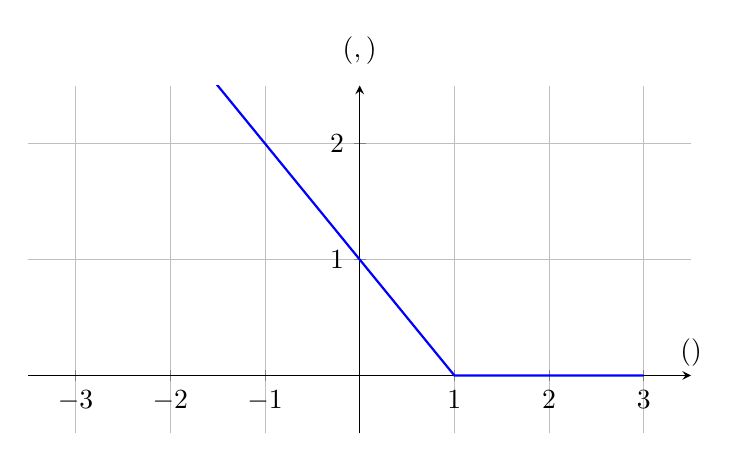
\begin{tikzpicture}
    \begin{axis}[
        axis lines=middle,
        xlabel={$\truelabel\hypothesis(\featurevec)$},
        ylabel={$\lossfunc{(\featurevec,\truelabel)}{\hypothesis}$},
 	xlabel style={at={(axis description cs:1.,0.3)}, anchor=north},  % Adjusted to be relative to axis end
        ylabel style={at={(axis description cs:0.5,1.1)}, anchor=center}, % Corrected to vertical position, rotated for readability
        xmin=-3.5, xmax=3.5,
        ymin=-0.5, ymax=2.5,
        xtick={-3, -2, -1, 0, 1, 2, 3},
        ytick={0, 1, 2},
        domain=-3:3,
        samples=100,
        width=10cm, height=6cm,
        grid=both,
        major grid style={line width=.2pt, draw=gray!50},
        minor grid style={line width=.1pt, draw=gray!20},
        legend pos=south west % Positions legend at the bottom left
    ]
        \addplot[blue, thick] {max(0, 1-x)};
     %   \addlegendentry{$\max(0, 1-x)$}
    \end{axis}
\end{tikzpicture}
	%	\end{figure} 
		\end{center}
	    A regularized variant of the hinge \gls{loss} is used by the \gls{svm} \cite{LampertNowKernel}. 	    
		},first={hinge loss},text={hinge loss}}

\newglossaryentry{iidasspt}{name={independent and identically distributed assumption (i.i.d.\ assumption)}, description={The \gls{iid} 
		assumption\index{independent and identically distributed assumption (i.i.d.\ assumption)} interprets \gls{datapoint}s of a \gls{dataset} as the 
		\gls{realization}s of \gls{iid} \gls{rv}s.},first={independent and identically distributed assumption (i.i.d.\ assumption)},text={i.i.d.\ assumption} }

\newglossaryentry{hypospace}{name={hypothesis space}, description={Every\index{hypothesis space} 
		practical \gls{ml} method uses a \gls{hypothesis} space (or \gls{model}) $\hypospace$. The \gls{hypothesis} space 
		of an \gls{ml} method is a subset of all possible maps from the \gls{featurespace} to the \gls{labelspace}. 
		The design choice of the \gls{hypothesis} space should take into account available computational resources and 
		\gls{statasp}. If the computational infrastructure allows for efficient matrix operations, and there 
		is an (approximately) linear relation between a set of \gls{feature}s and a \gls{label}, a useful choice for the 
		\gls{hypothesis} space might be the \gls{linmodel}.},first={hypothesis space},text={hypothesis space} }
	
\newglossaryentry{model}{name={model}, description={In\index{model} the context of \gls{ml} methods, 
		the term model typically refers to the \gls{hypospace} employed by an 
		\gls{ml} method \cite{ShalevMLBook,MLBasics}.},first={model},text={model} }

\newglossaryentry{modelparams}{name={model parameters}, 
	description={\Gls{model} \gls{parameters}\index{model parameters} are quantities that 
	are used to select a specific \gls{hypothesis} map from a \gls{model}. 
	We can think of a list of \gls{model} \gls{parameters} as a unique identifier for a \gls{hypothesis} 
	map, similar to how a social security number identifies a person in Finland.},
	first={model parameters},text={model parameters} }

\newglossaryentry{ai}{name={artificial intelligence (AI)}, description={
		AI\index{artificial intelligence (AI)} refers to systems that behave rationally in the sense of 
		maximizing a long-term \gls{reward}. The \gls{ml}-based approach to AI is to train a \gls{model} for  
		predicting optimal actions. These predictions are computed from observations about the state of the 
		environment. The choice of \gls{lossfunc} sets AI applications apart from more basic \gls{ml} applications. 
		AI systems rarely have access to a labeled \gls{trainset} that allows the average \gls{loss} to be measured for any possible choice of \gls{modelparams}. 
		Instead, AI systems use observed \gls{reward} signals to obtain a (point-wise) estimate for the 
		\gls{loss} incurred by the current choice of \gls{modelparams}.},first={AI},text={AI} }

\newglossaryentry{reward}{name={reward}, description={A reward refers to some\index{reward} observed 
		(or measured) quantity that allows us to estimate the \gls{loss} incurred by the \gls{prediction} 
		(or decision) of a \gls{hypothesis} $\hypothesis(\featurevec)$. For example, in an 
		\gls{ml} application to self-driving vehicles, $\hypothesis(\featurevec)$ could represent 
		the current steering direction of a vehicle. We could construct a reward from the 
		measurements of a collision sensor that indicate if the vehicle is moving towards 
		an obstacle. We define a low reward for the steering direction 
	$\hypothesis(\featurevec)$ if the vehicle moves dangerously towards an obstacle.},
	first={reward}, text={reward}} 

\newglossaryentry{hardclustering}{name={hard clustering}, description={Hard \gls{clustering}\index{hard clustering} 
		refers to the task of partitioning a given set of \gls{datapoint}s into (a few) non-overlapping \gls{cluster}s. 
		The most widely used hard \gls{clustering} method is \gls{kmeans}.},first={hard clustering},text={hard clustering} }
	
\newglossaryentry{softclustering}{name={soft clustering}, description={Soft \gls{clustering}\index{soft clustering} 
		refers to the task of partitioning a given set of \gls{datapoint}s into (a few) overlapping \gls{cluster}s. 
		Each \gls{datapoint} is assigned to several different \gls{cluster}s with varying degrees of belonging. Soft \gls{clustering} 
		methods determine the \gls{dob} (or soft \gls{cluster} assignment) for each \gls{datapoint} and each \gls{cluster}.
		A principled approach to soft \gls{clustering} is by interpreting \gls{datapoint}s as \gls{iid} \gls{realization}s 
		of a \gls{gmm}. We then obtain a natural choice for the \gls{dob} as the conditional 
		\gls{probability} of a \gls{datapoint} belonging to a specific mixture component.},first={soft clustering},text={soft clustering} }
	
\newglossaryentry{clustering}{name={clustering}, description={Clustering\index{clustering} methods decompose a given 
		set of \gls{datapoint}s into a few subsets, which are referred to as \gls{cluster}s. 
		Each \gls{cluster} consists of \gls{datapoint}s that are more similar to each 
		other than to \gls{datapoint}s outside the \gls{cluster}. Different clustering methods 
		use different measures for the similarity between \gls{datapoint}s and different 
		forms of \gls{cluster} representations. The clustering method \gls{kmeans} uses the 
		average \gls{feature} vector (cluster \gls{mean}) of a \gls{cluster} as its representative. 
		A popular \gls{softclustering} method based on \gls{gmm} represents 
		a \gls{cluster} by a \gls{mvndist}.},first={clustering},text={clustering} }
	
\newglossaryentry{cluster}{name={cluster}, description={A\index{cluster} cluster is a subset of 
		\gls{datapoint}s that are more similar to each other than to the \gls{datapoint}s outside the cluster. 
		The quantitative measure of similarity between \gls{datapoint}s is a design choice. If \gls{datapoint}s 
		are characterized by Euclidean \gls{featurevec}s $\featurevec \in \mathbb{R}^{\nrfeatures}$, 
		we can define the similarity between two \gls{datapoint}s via the Euclidean distance between 
		their \gls{featurevec}s.},first={cluster},text={cluster} }

%\newglossaryentry{softclustering}{name={soft clustering}, description={Soft clustering methods determine, for each \gls{datapoint} within a dataset, 
%		a soft cluster assignment or the degree of belonging to a particular cluster.},first={soft clustering},text={soft clustering} }


\newglossaryentry{huberloss}{name={Huber loss}, description={The\index{Huber loss} 
		Huber \gls{loss} unifies the \gls{sqerrloss} and the \gls{abserr}.},first={Huber loss},text={Huber loss} }

\newglossaryentry{svm}{name={support vector machine (SVM)}, description={The\index{support vector machine (SVM)} 
		SVM is a binary \gls{classification} method that 
		learns a linear \gls{hypothesis} map. Thus, like \gls{linreg} and \gls{logreg}, 
		it is also an instance of \gls{erm} for the \gls{linmodel}. However, the 
		SVM uses a different \gls{lossfunc} from the one used in those methods. As illustrated in 
		Figure \ref{fig_svm_gls_dict}, it aims to maximally separate \gls{datapoint}s from 
		the two different classes in the \gls{featurespace} (i.e., \gls{maximum} margin principle). 
		Maximizing this separation is equivalent to minimizing a regularized 
		variant of the \gls{hingeloss} \eqref{equ_hinge_loss_gls_dict} \cite{LampertNowKernel,Cristianini_Shawe-Taylor_2000,BishopBook}.
		\begin{figure}[H]
			\begin{center}
				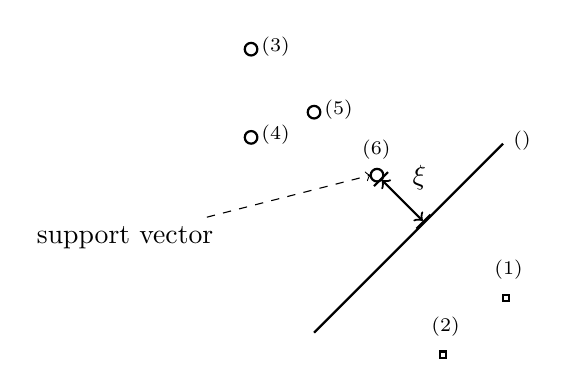
\begin{tikzpicture}[auto,scale=0.8]
					%\draw [thick] (0,-3) rectangle (4,4) node [anchor=east,above] {$\featurespace$} ;
					\draw [thick] (1,2) circle (0.1cm)node[anchor=west] {\hspace*{0mm}$\featurevec^{(5)}$};
					\draw [thick] (0,1.6) circle (0.1cm)node[anchor=west] {\hspace*{0mm}$\featurevec^{(4)}$};
					\draw [thick] (0,3) circle (0.1cm)node[anchor=west] {\hspace*{0mm}$\featurevec^{(3)}$};
					\draw [thick] (2,1) circle (0.1cm)node[anchor=east,above] {\hspace*{0mm}$\featurevec^{(6)}$};
					\node[] (B) at (-2,0) {support vector};
					\draw[->,dashed] (B) to (1.9,1) ; 
					\draw [|<->|,thick] (2.05,0.95)  -- (2.75,0.25)node[pos=0.5] {$\xi$} ; 
					\draw [thick] (1,-1.5) -- (4,1.5) node [right] {$\hypothesis^{(\weights)}$} ; 
					\draw [thick] (3,-1.9) rectangle ++(0.1cm,0.1cm) node[anchor=west,above]  {\hspace*{0mm}$\featurevec^{(2)}$};
					\draw [thick] (4,.-1) rectangle ++(0.1cm,0.1cm) node[anchor=west,above] {\hspace*{0mm}$\featurevec^{(1)}$};
				\end{tikzpicture}
				\caption{The \gls{svm} learns a \gls{hypothesis} (or \gls{classifier}) $\hypothesis^{(\weights)}$ with 
					minimal average soft-margin \gls{hingeloss}. Minimizing this \gls{loss} is equivalent 
					to maximizing the margin $\xi$ between the \gls{decisionboundary} of $\hypothesis^{(\weights)}$ 
					and each class of the \gls{trainset}.}
				\label{fig_svm_gls_dict}
			\end{center}
		\end{figure}
		The above basic variant of SVM is only useful if the \gls{datapoint}s from different categories can be  
		(approximately) linearly separated. For an \gls{ml} application where the categories are not 
		%linearly separable based on the the original (raw) \gls{feature}s it is possible to apply the SVM 
		%to transformed \gls{feature}s. These transformed \gls{feature}s can be obtained by applying a \gls{featuremap} 
		derived from a \gls{kernel}.
},first={support vector machine (SVM)},text={SVM} }

\newglossaryentry{eigenvalue}{name={eigenvalue}, description={We\index{eigenvalue} refer to a 
		number $\lambda \in \mathbb{R}$ as an eigenvalue of a square matrix $\mathbf{A} \in \mathbb{R}^{\featuredim \times \featuredim}$ 
		if there is a non-zero vector $\vx \in \mathbb{R}^{\featuredim} \setminus \{ \mathbf{0} \}$ such that $\mathbf{A} \vx = \lambda \vx$. },first={eigenvalue},text={eigenvalue} }
	
\newglossaryentry{eigenvector}{name={eigenvector}, description={An\index{eigenvector} 
		eigenvector of a matrix $\mathbf{A} \in \mathbb{R}^{\featuredim \times \featuredim}$ 
		is a non-zero vector $\vx \in \mathbb{R}^{\featuredim} \setminus \{ \mathbf{0} \}$ 
		such that $\mathbf{A} \vx = \lambda \vx$ with some \gls{eigenvalue} $\lambda$.},first={eigenvector},text={eigenvector} }

\newglossaryentry{evd}{name={eigenvalue decomposition (EVD)}, 
	description={The\index{eigenvalue decomposition (EVD)} \gls{eigenvalue} 
		decomposition for a square matrix $\mA \in \mathbb{R}^{\dimlocalmodel \times \dimlocalmodel}$ 
		is a factorization of the form 
		$$\mA = \mathbf{V} {\bm \Lambda} \mathbf{V}^{-1}.$$ 
		The columns of the matrix $\mV = \big( \vv^{(1)},\ldots,\vv^{(\dimlocalmodel)} \big)$ are the 
		\gls{eigenvector}s of the matrix $\mV$. The diagonal matrix 
		${\bm \Lambda} = {\rm diag} \big\{ \eigval{1},\ldots,\eigval{\dimlocalmodel} \big\}$ 
		contains the \gls{eigenvalue}s $\eigval{\featureidx}$ corresponding to the \gls{eigenvector}s $\vv^{(\featureidx)}$. 
		Note that the above decomposition exists only if the matrix $\mA$ is diagonalizable.},first={eigenvalue decomposition (EVD)},text={EVD} }

\newglossaryentry{svd}{name={singular value decomposition (SVD)}, 
  	description={The\index{singular value decomposition (SVD)} SVD  
  		for a matrix $\mA \in \mathbb{R}^{\samplesize \times \dimlocalmodel}$ 
		is a factorization of the form 
		$$\mA = \mathbf{V} {\bm \Lambda} \mathbf{U}^{T},$$ 
		with orthonormal matrices $\mV \in \mathbb{R}^{\samplesize \times \samplesize}$ 
		and $\mU \in \mathbb{R}^{\dimlocalmodel \times \dimlocalmodel}$ \cite{GolubVanLoanBook}. 
		The matrix ${\bm \Lambda} \in \mathbb{R}^{\samplesize \times \dimlocalmodel}$ is 
		only non-zero along the main diagonal, whose entries $\Lambda_{\featureidx,\featureidx}$ 
		are non-negative and referred to as singular values.
	},first={singular value decomposition (SVD)},text={SVD} }


\newglossaryentry{tv}{name={total variation}, description={See \gls{gtv}\index{total variation}.},
	first={total variation},text={total variation} }

 \newglossaryentry{cvxclustering}{name={convex clustering}, 
 	description={Consider\index{convex clustering} a \gls{dataset} 
 	$\featurevec^{(1)},\ldots,\featurevec^{(\samplesize)} \in \mathbb{R}^{\nrfeatures}$. 
 	\Gls{convex} \gls{clustering} learns vectors $\weights^{(1)},\ldots,\weights^{(\samplesize)}$ by 
 	minimizing 
 	$$ \sum_{\sampleidx=1}^{\samplesize} \normgeneric{\featurevec^{(\sampleidx)} - \weights^{(\sampleidx)}}{2}^2 + 
 	\regparam \sum_{\nodeidx,\nodeidx' \in \nodes} \normgeneric{\weights^{(\nodeidx)} - \weights^{(\nodeidx')}}{p}.$$ 
	Here, $ \normgeneric{\vu}{p} \defeq \big( \sum_{\featureidx=1}^{\dimlocalmodel} |u_{\featureidx}|^{p} \big)^{1/p}$ 
	denotes the $p$-\gls{norm} (for $p\geq1$).  
	It turns out that many of the optimal vectors $\widehat{\weights}^{(1)},\ldots,\widehat{\weights}^{(\samplesize)}$ 
	coincide. A \gls{cluster} then consists of those \gls{datapoint}s $\sampleidx \in \{1,\ldots,\samplesize\}$ 
	with identical $\widehat{\weights}^{(\sampleidx)}$ \cite{JMLR:v22:18-694,Pelckmans2005}. 
 	  },
 		first={convex clustering},text={convex clustering} }


\newglossaryentry{gdmethods}{name={gradient-based methods}, 
	description={\Gls{gradient}-based\index{gradient-based methods} 
		methods are iterative techniques for finding the \gls{minimum} (or \gls{maximum}) 
		of a \gls{differentiable} \gls{objfunc} of the \gls{modelparams}. These 
		methods construct a sequence of approximations to an optimal choice for 
		\gls{modelparams} that results in a \gls{minimum} (or \gls{maximum}) value of the \gls{objfunc}. 
		As their name indicates, \gls{gradient}-based methods use the \gls{gradient}s of the \gls{objfunc} 
		evaluated during previous iterations to construct new, (hopefully) improved \gls{modelparams}. 
		One important example of a \gls{gradient}-based method is \gls{gd}.},
		first={gradient-based methods},text={gradient-based methods} }

\newglossaryentry{sgd}{name={subgradient descent}, description={\Gls{subgradient}\index{subgradient descent} 
		descent is a \gls{generalization} of \gls{gd} that does not require differentiability of the 
		function to be minimized. This \gls{generalization} is obtained by replacing the concept 
		of a \gls{gradient} with that of a \gls{subgradient}. Similar to \gls{gradient}s, also \gls{subgradient}s 
		allow us to construct local approximations of an \gls{objfunc}. The \gls{objfunc} 
		might be the \gls{emprisk} $\emperror\big( \hypothesis^{(\weights)} \big| \dataset \big)$ viewed 
		as a function of the \gls{modelparams} $\weights$ that select a \gls{hypothesis} $\hypothesis^{(\weights)} \in \hypospace$.},first={subgradient descent},text={subgradient descent} }
	
\newglossaryentry{stochGD}{name={stochastic gradient descent (SGD)}, description={Stochastic\index{stochastic gradient descent (SGD)} 
		\gls{gd} is obtained from \gls{gd} by replacing the \gls{gradient} of the \gls{objfunc} 
		with a stochastic approximation. A main application of stochastic \gls{gd} 
		is to train a parametrized \gls{model} via \gls{erm} on a \gls{trainset} $\dataset$ that 
		is either very large or not readily available (e.g., when \gls{datapoint}s are stored 
		in a database distributed all over the planet). To evaluate the \gls{gradient} of the 
		\gls{emprisk} (as a function of the \gls{modelparams} $\weights$), 
		we need to compute a sum $\sum_{\sampleidx=1}^{\samplesize} \nabla_{\weights} \lossfunc{\datapoint^{(\sampleidx)}}{\weights}$  
		over all \gls{datapoint}s in the \gls{trainset}. We obtain a stochastic 
		approximation to the \gls{gradient} by replacing the sum $\sum_{\sampleidx=1}^{\samplesize} \nabla_{\weights} \lossfunc{\datapoint^{(\sampleidx)}}{\weights}$ 
		with a sum $\sum_{\sampleidx \in \batch} \nabla_{\weights} \lossfunc{\datapoint^{(\sampleidx)}}{\weights}$ 
		over a randomly chosen subset $\batch \subseteq \{1,\ldots,\samplesize\}$ (see Figure \ref{fig_sgd_approx_dict}). 
		We often refer to these randomly chosen \gls{datapoint}s as a \gls{batch}. 
		The \gls{batch} size $|\batch|$ is an important parameter of stochastic \gls{gd}. 
		Stochastic \gls{gd} with $|\batch|> 1$ is referred to as mini-\gls{batch} stochastic \gls{gd} \cite{Bottou99}. 		
		\begin{figure}[H]
			\centering
			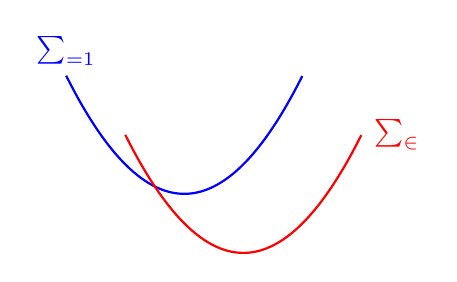
\begin{tikzpicture}[scale=1.5, >=stealth]
% Axes
				%\draw[->] (-1, 0) -- (4, 0) node[right] {$w$};
				%\draw[->] (0, -0.5) -- (0, 4) node[above] {};
% First quadratic function: f(w)
				\draw[thick, blue, domain=0.5:2.5, samples=100] plot (\x, {(\x-1.5)^2 + 1});
				\node[blue,above] at (0.5, 2) {$\sum_{\sampleidx=1}^{\samplesize}$};
% Second quadratic function: f'(w)
				\draw[thick, red, domain=1:3, samples=100] plot (\x, {(\x-2)^2 + 0.5});
				\node[red] at (3.3, 1.5) {$\sum_{\sampleidx \in \batch}$};
% Labels
			\end{tikzpicture}
		\caption{Stochastic \gls{gd} for \gls{erm} approximates the \gls{gradient} 
		$\sum_{\sampleidx=1}^{\samplesize} \nabla_{\weights} \lossfunc{\datapoint^{(\sampleidx)}}{\weights}$ 
		by replacing the 
		sum over all \gls{datapoint}s in the \gls{trainset} (indexed by $\sampleidx=1,\ldots,\samplesize$) 
		with a sum over a randomly chosen subset $\batch \subseteq \{1,\ldots,\samplesize\}$.\label{fig_sgd_approx_dict}}
		\end{figure}
},first={stochastic gradient descent (SGD)},text={SGD} }


\newglossaryentry{onlineGD}{name={online gradient descent (online GD)}, description={
Consider \index{online gradient descent (online GD)} an \gls{ml} method that learns \gls{modelparams} 
$\weights$ from some \gls{paramspace} $\paramspace \subseteq \mathbb{R}^{\dimlocalmodel}$. 
The learning process uses \gls{datapoint}s $\datapoint^{(\timeidx)}$ that arrive at consecutive time-instants $\timeidx=1,2,\ldots$. 
Let us interpret the \gls{datapoint}s $\datapoint^{(\timeidx)}$ as \gls{iid} copies 
of an \gls{rv} $\datapoint$. The \gls{risk} $\expect\{ \lossfunc{\datapoint}{\weights} \}$ of a 
\gls{hypothesis} $\hypothesis^{(\weights)}$ can then (under mild conditions) be obtained as the limit 
$\lim_{T\rightarrow \infty} (1/T)\sum_{\timeidx=1}^{T} \lossfunc{\datapoint^{(\timeidx)}}{\weights}$. 
We might use this limit as the \gls{objfunc} for learning the \gls{modelparams} $\weights$. 
Unfortunately, this limit can only be evaluated if we wait infinitely long in order to collect all \gls{datapoint}s. 
Some \gls{ml} applications require methods that learn online: as soon as a new \gls{datapoint} $\datapoint^{(\timeidx)}$ 
arrives at time $\timeidx$, we update the current \gls{modelparams} $\weights^{(\timeidx)}$. Note that 
the new \gls{datapoint} $\datapoint^{(\timeidx)}$ contributes the component $\lossfunc{\datapoint^{(\timeidx)}}{\weights}$ 
to the \gls{risk}. As its name suggests, online \gls{gd} updates $\weights^{(\timeidx)}$ via a (projected) \gls{gradstep}
\begin{equation} 
\label{equ_def_ogd_dict}
 \weights^{(\timeidx+1)} \defeq \projection{\paramspace}{\weights^{(\timeidx)} - \lrate_{\timeidx} \nabla_{\weights} \lossfunc{\datapoint^{(\timeidx)}}{\weights}}. 
\end{equation} 
Note that \eqref{equ_def_ogd_dict} is a \gls{gradstep} for the current component $\lossfunc{\datapoint^{(\timeidx)}}{\cdot}$ 
of the \gls{risk}. The update \eqref{equ_def_ogd_dict} ignores all the previous components $\lossfunc{\datapoint^{(\timeidx')}}{\cdot}$, 
for $\timeidx' < \timeidx$. It might therefore happen that, compared to $\weights^{(\timeidx)}$, the updated \gls{modelparams} 
$\weights^{(\timeidx+1)}$ increase the retrospective average \gls{loss} $\sum_{\timeidx'=1}^{\timeidx-1} \lossfunc{\datapoint^{(\timeidx')}}{\cdot}$. 
However, for a suitably chosen \gls{learnrate} $\lrate_{\timeidx}$, online \gls{gd} can be shown 
to be optimal in practically relevant settings. By optimal, we mean that the \gls{modelparams} 
$\weights^{(T+1)}$ delivered by online \gls{gd} after observing $T$ \gls{datapoint}s $\datapoint^{(1)},\ldots, \datapoint^{(T)}$ 
are at least as good as those delivered by any other learning method \cite{HazanOCO,GDOptimalRakhlin2012}. 
\begin{figure}[H]
	\begin{center}
\begin{tikzpicture}[x=1.5cm,scale=1.5, every node/.style={font=\footnotesize}]
	% Axes
	\draw[->] (0.5, 0) -- (5.5, 0) node[below] {};
	%\draw[->] (0, -0.5) -- (0, 3) node[left] {Value};
	% Labels for time steps
	\foreach \x in {1, 2, 3, 4, 5} {
		\draw (\x, 0.1) -- (\x, -0.1) node[below] {$t=\x$};
	}
	% Data points (black circles)
	\foreach \x/\y in {1/2.5, 2/1.8, 3/2.3, 4/1.5, 5/2.0} {
		\fill[black] (\x, \y) circle (2pt) node[above right] {$\datapoint^{(\x)}$};
	}
	% Model parameters (blue circles)
	\foreach \x/\y in {1/1.0, 2/1.6, 3/1.8, 4/2.2, 5/1.9} {
		\fill[blue] (\x, \y) circle (2pt) node[below left] {$\weights^{(\x)}$};
	}
	% Connecting lines (model tracking data)
	\foreach \x/\y/\z in {1/2.5/1.0, 2/1.8/1.6, 3/2.3/2.0, 4/1.5/1.8, 5/2.0/1.9} {
		\draw[dashed, gray] (\x, \y) -- (\x, \z);
	}
	% Legend
	% \node[draw, fill=white] at (4.5, 2.7) {
	% 	\begin{tabular}{@{}ll@{}}
	% 		\textcolor{black}{$\bullet$} & Data Point ($d_t$) \\
	% 		\textcolor{blue}{$\bullet$} & Model Parameter ($\theta_t$) \\
	% 		\textcolor{gray}{\rule{1cm}{0.5pt}} & Gradient Update
	% 	\end{tabular}
	%};
	\end{tikzpicture}
\end{center} 
\caption{An instance of online \gls{gd} that updates the \gls{modelparams} $\weights^{(\timeidx)}$ 
using the \gls{datapoint} $\datapoint^{(\timeidx)} = \feature^{(\timeidx)}$ arriving at time $\timeidx$. 
This instance uses the \gls{sqerrloss} $\lossfunc{\datapoint^{(\timeidx)}}{\weight} = (\feature^{(\timeidx)} - \weight)^{2}$.
}
\end{figure}},
first={online gradient descent (online GD)},text={online GD}}

\newglossaryentry{pca}{name={principal component analysis (PCA)}, description={PCA\index{principal component analysis (PCA)} 
		determines a linear \gls{featuremap} such that the new \gls{feature}s 
		allow us to reconstruct the original \gls{feature}s with the \gls{minimum} reconstruction error \cite{MLBasics}.},first={principal component analysis (PCA)},text={PCA} }
	
\newglossaryentry{loss}{name={loss}, description={\gls{ml}\index{loss} methods use a 
		\gls{lossfunc} $\lossfunc{\datapoint}{\hypothesis}$ to measure the error incurred 
		by applying a specific \gls{hypothesis} to a specific \gls{datapoint}. With a
		slight abuse of notation, we use the term loss for both the \gls{lossfunc} $\loss$ 
		itself and the specific value $\lossfunc{\datapoint}{\hypothesis}$, for a \gls{datapoint} $\datapoint$ 
		and \gls{hypothesis} $\hypothesis$.},first={loss},text={loss} }

\newglossaryentry{lossfunc}{name={loss function}, description={A\index{loss function} \gls{loss} function is a map 
		$$\lossfun: \featurespace \times \labelspace \times \hypospace \rightarrow \mathbb{R}_{+}: \big( \big(\featurevec,\truelabel\big),
		 \hypothesis\big) \mapsto  \lossfunc{(\featurevec,\truelabel)}{\hypothesis}.$$
		It assigns a non-negative real number (i.e., the \gls{loss}) $\lossfunc{(\featurevec,\truelabel)}{\hypothesis}$
		to a pair that consists of a \gls{datapoint}, with \gls{feature}s $\featurevec$ 
		and \gls{label} $\truelabel$, and a \gls{hypothesis} $\hypothesis \in \hypospace$. The 
		value $\lossfunc{(\featurevec,\truelabel)}{\hypothesis}$ quantifies the discrepancy 
		between the true \gls{label} $\truelabel$ and the \gls{prediction} $\hypothesis(\featurevec)$. 
		Lower (closer to zero) values $\lossfunc{(\featurevec,\truelabel)}{\hypothesis}$ indicate a smaller 
		discrepancy between \gls{prediction} $\hypothesis(\featurevec)$ and \gls{label} $\truelabel$. 
		Figure \ref{fig_loss_function_gls_dict} depicts a \gls{loss} function for a given \gls{datapoint}, 
		with \gls{feature}s $\featurevec$ and \gls{label} $\truelabel$, as a function of the \gls{hypothesis} $\hypothesis \in \hypospace$. 
		\begin{figure}[H]
			\begin{center}
				\begin{tikzpicture}[scale = 0.7]
					\begin{axis}
						[%grid, 
						axis x line=center,
						axis y line=center,
						%	xtick={-2,-1,...,2},
						%	ytick={0,1,...,2},
						xlabel={},
						%	ylabel={\hspace*{3mm} loss $\lossfun$},
						xlabel style={below right},
						ylabel style={above right},
						xtick=\empty,
						ytick=\empty,
						xmin=-4,
						xscale = 1.4, 
						xmax=4,
						ymin=-0.5,
						ymax=2.5
						]
						\addplot [smooth, ultra thick] table [x=a, y=b, col sep=comma] {assets/logloss.csv};    
					\end{axis}
					\node [above] at (1,5) {$\lossfunc{(\featurevec,\truelabel)}{\hypothesis}$};
					\node [above] at (10,1) {\gls{hypothesis} $\hypothesis$};
						\node [right] at (4,6) {\gls{loss}};
				\end{tikzpicture}
			\end{center}
			\vspace*{-7mm}
			\caption{Some \gls{loss} function $\lossfunc{(\featurevec,\truelabel)}{\hypothesis}$ for a fixed \gls{datapoint}, with 
				\gls{featurevec} $\featurevec$ and \gls{label} $\truelabel$, and a varying \gls{hypothesis} $\hypothesis$. 
				\gls{ml} methods try to find (or learn) a \gls{hypothesis} that incurs minimal \gls{loss}.}
			\label{fig_loss_function_gls_dict}
	\end{figure}
 },first={loss function},text={loss function} }

\newglossaryentry{decisiontree}{name={decision tree}, description={A\index{decision tree} 
		decision tree is a flow-chart-like representation of a \gls{hypothesis} map $\hypothesis$. 
		More formally, a decision tree is a directed \gls{graph} containing a root node that reads 
		in the \gls{featurevec} $\featurevec$ of a \gls{datapoint}. The root node then forwards 
		the \gls{datapoint} to one of its children nodes based on some elementary test on the \gls{feature}s $\featurevec$. 
		If the receiving child node is not a leaf node, i.e., it has itself children nodes, 
	  it represents another test. Based on the test result, the \gls{datapoint} is forwarded 
	   to one of its descendants. This testing and forwarding of the \gls{datapoint} is continued 
	  until the \gls{datapoint} ends up in a leaf node (having no children nodes). 
\begin{figure}[H]
\begin{minipage}{.45\textwidth}
	\scalebox{1}{
\begin{tikzpicture}
%	% Root node
	\node[fill=black, circle, inner sep=2pt, label=above:{$\| \featurevec-\mathbf{u} \| \leq \varepsilon$?}] (A) {};	
%	% Left child (h1)
	\node[fill=black, circle, inner sep=2pt, below left=1.5cm and 1cm of A, label=left:{$\hypothesis(\featurevec) = \predictedlabel_1$}] (B) {};
	% Right child (next question)
	\node[fill=black, circle, inner sep=2pt, below right=1.5cm and 1cm of A, label=right:{$\| \featurevec - \mathbf{v} \| \leq \varepsilon$?}] (C) {};
%	% Left child of C (h2)
	\node[fill=black, circle, inner sep=2pt, below left=1.5cm and 1cm of C, label=left:{$\hypothesis(\featurevec) = \predictedlabel_2$}] (D) {};
	% Right child of C (h3)
	\node[fill=black, circle, inner sep=2pt, below right=1.5cm and 1cm of C, label=right:{$\hypothesis(\featurevec) =\predictedlabel_3$}] (E) {};
%	% Arrows
	\draw[line width=1.5pt, ->] (A) -- (B) node[midway, left] {no};
	\draw[line width=1.5pt, ->] (A) -- (C) node[midway, right] {yes};
	\draw[line width=1.5pt, ->] (C) -- (D) node[midway, left] {no};
	\draw[line width=1.5pt, ->] (C) -- (E) node[midway, right] {yes};
\end{tikzpicture}
	}
\end{minipage}	
\hspace*{15mm}
\begin{minipage}{.45\textwidth}
	\hspace*{15mm}
	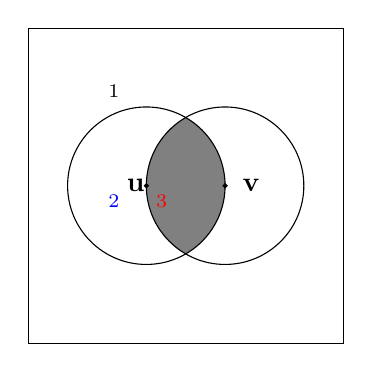
\begin{tikzpicture}
		\draw (-2,2) rectangle (2,-2);
		\begin{scope}
			\clip (-0.5,0) circle (1cm);
			\clip (0.5,0) circle (1cm);
			\fill[color=gray] (-2,1.5) rectangle (2,-1.5);
		\end{scope}
		\draw (-0.5,0) circle (1cm);
		\draw (0.5,0) circle (1cm);
		\draw[fill] (-0.5,0) circle [radius=0.025];
		\node [below right, red] at (-0.5,0) {$\predictedlabel_{3}$};
		\node [below left, blue] at (-0.7,0) {$\predictedlabel_{2}$};
		\node [above left] at (-0.7,1) {$\predictedlabel_{1}$};
		\node [left] at (-0.4,0) {$\mathbf{u}$};
		\draw[fill] (0.5,0) circle [radius=0.025];
		\node [right] at (0.6,0) {$\mathbf{v}$};
	\end{tikzpicture}
\end{minipage}
	\caption{Left: A decision tree is a flow-chart-like representation of a piece-wise constant \gls{hypothesis} $\hypothesis: \featurespace \rightarrow \mathbb{R}$.  Each piece is a \gls{decisionregion} $\decreg{\predictedlabel} \defeq \big\{ \featurevec \in  \featurespace: \hypothesis(\featurevec) = \predictedlabel \big\}$. 
		The depicted decision tree can be applied to numeric \gls{featurevec}s, i.e., $\featurespace \subseteq \mathbb{R}^{\dimlocalmodel}$. It is  parametrized by the threshold $\varepsilon>0$ and the vectors $\vu, \vv \in \mathbb{R}^{\dimlocalmodel}$. 
		Right: A decision tree partitions  
		the \gls{featurespace} $\featurespace$ into \gls{decisionregion}s. Each \gls{decisionregion}  
		$\decreg{\hat{\truelabel}} \!\subseteq\!\featurespace$ corresponds to a specific leaf node in the decision tree.}
	\label{fig_decision_tree}
\end{figure} 
	  }
	  ,first={decision tree},text={decision tree} }

%\newglossaryentry{API} 
%{
%	name={application programming interface (API)},
%	description={An\index{application programming interface} application programming 
%		interface (API) is a precise specification of the services and resources 
%		offered by software or hardware implementing that API.},
%	first={application programming interface (API)},
%	text={API}
%}


\newglossaryentry{API} 
{name={application programming interface (API)},
		description={
			An \index{application programming interface (API)} API is a formal mechanism for enabling 
			software components to interact in a structured manner \cite{RestfulBook2013}. In the 
			context of \gls{ml}, APIs are frequently used to make a trained \gls{ml} \gls{model} 
			accessible to different types of users. These users, which can be other computers 
			or humans, can request a \gls{prediction} for the \gls{label} of a \gls{datapoint} by 
			providing its \gls{feature}s. The internal structure of the \gls{ml} 
			\gls{model} remains hidden from the user. For instance, consider a trained \gls{ml} \gls{model}  
			$\widehat{\hypothesis}(\feature) \defeq  2 \feature+1$. An API enables a user to 
			submit the \gls{feature} value $\feature=3$ and obtain the response $\widehat{\hypothesis}(3)=7$ 
			without knowledge of the detailed structure of the \gls{ml} \gls{model} or its training. 
			In practice, the \gls{ml} \gls{model} is typically hosted on a computer (i.e., a server) connected to the internet. 
			Another computer (i.e., a client) sends the \gls{feature}s of a \gls{datapoint} to the 
			server, which then computes $\widehat{\hypothesis}(\featurevec)$ and returns the 
			result to the external system. APIs help to modularize the development of 
			\gls{ml} applications by decoupling specific tasks. For instance, one team can 
			focus on developing and training the \gls{model}, while another team handles 
			user interaction and integration of the \gls{model} into applications.
			},
		first={application programming interface (API)},
		text={API}
}


\newglossaryentry{hilbertspace}{name={Hilbert space},description={A\index{Hilbert space} 
		Hilbert space is a linear vector space equipped with an inner product between 
		pairs of vectors. One important example of a Hilbert space is the \gls{euclidspace} 
		$\mathbb{R}^{\featuredim}$, for some dimension $\featuredim$, which consists of 
		Euclidean vectors $\vu = \big(u_{1},\ldots,u_{\featurelen}\big)^{T}$ along with the inner 
		product $\vu^{T} \vv$.},first={Hilbert space},text={Hilbert space}}



\newglossaryentry{sample}{name={sample},description={A\index{sample} 
		finite sequence (or list) of \gls{datapoint}s $\datapoint^{(1)},\ldots,\datapoint^{(m)}$ that 
		is obtained or interpreted as the \gls{realization} of $\samplesize$ \gls{iid} \gls{rv}s 
		with a common \gls{probdist} $p(\datapoint)$. The length $\samplesize$ of 
		the sequence is referred to as the \gls{samplesize}.},first={sample},text={sample}}
	
\newglossaryentry{samplesize}
{name=sample size,
	description={The\index{sample size} number of individual \gls{datapoint}s 
		contained in a \gls{dataset}.},first={sample size},text={sample size}
}

\newglossaryentry{ann}{
	name={artificial neural network (ANN)},
	description={An\index{artificial neural network (ANN)} ANN 
		is a graphical (signal-flow) representation of a function that maps 
		\gls{feature}s of a \gls{datapoint} at its input to a \gls{prediction} 
		for the corresponding \gls{label} at its output. The fundamental unit of an 
		ANN is the artificial neuron, which applies an \gls{actfun} to its 
		weighted inputs. The outputs of these neurons serve as inputs for other neurons, 
		forming interconnected layers.},
	first={artificial neural network (ANN)},
	text={ANN}
}


\newglossaryentry{randomforest}
{name=random forest,
	description={A\index{random forest} random forest is a set (or ensemble) of different \gls{decisiontree}s. 
		Each of these \gls{decisiontree}s is obtained by fitting a perturbed copy of 
		the original \gls{dataset}.},first = {random forest}, text={random forest}
}

\newglossaryentry{bagging}{name={bagging},description={Bagging\index{bagging} (or bootstrap aggregation) 
		is a generic technique to improve (the robustness of) a given \gls{ml} method. The idea is to use the \gls{bootstrap} 
		to generate perturbed copies of a given \gls{dataset} and then to learn a separate \gls{hypothesis} for 
		each copy. We then predict the \gls{label} of a \gls{datapoint} by combining or aggregating the individual 
		\gls{prediction}s of each separate \gls{hypothesis}. For \gls{hypothesis} maps delivering numeric \gls{label} 
		values, this aggregation could be implemented by computing the average of individual \gls{prediction}s.},first={bootstrap aggregation (bagging)},text={bagging}}

\newglossaryentry{gd}{name={gradient descent (GD)},description={\Gls{gradient}\index{gradient descent (GD)} 
		descent is an iterative method for finding the \gls{minimum} of a \gls{differentiable} function $f(\weights)$ 
		of a vector-valued argument $\weights \in \mathbb{R}^{\featurelen}$. Consider a current guess or 
		approximation $\weights^{(\itercntr)}$ for the \gls{minimum} of the function $f(\weights)$. We would like to find a new (better) vector $\weights^{(\itercntr+1)}$ 
		that has a smaller objective value $f(\weights^{(\itercntr+1)}) < f\big(\weights^{(\itercntr)}\big)$ than 
		the current guess $\weights^{(\itercntr)}$. We can achieve this typically by using a \gls{gradstep}
		\begin{equation} 
			\label{equ_def_GD_step_dict}
			\weights^{(\itercntr\!+\!1)} = \weights^{(\itercntr)} - \lrate \nabla f(\weights^{(\itercntr)})
		\end{equation} 
		with a sufficiently small \gls{stepsize} $\lrate\!>\!0$. Figure \ref{fig_basic_GD_step_dict} illustrates the effect of 
		a single \gls{gradient} descent step \eqref{equ_def_GD_step_dict}.
		\begin{figure}[H]
			\begin{center}
				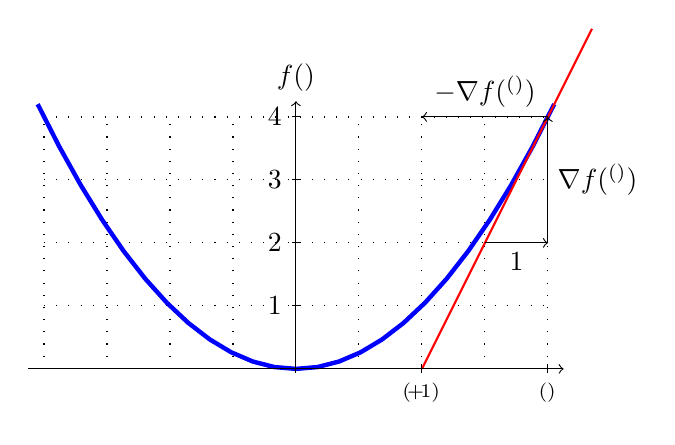
\begin{tikzpicture}[scale=0.8]
					\draw[loosely dotted] (-4,0) grid (4,4);
					\draw[blue, ultra thick, domain=-4.1:4.1] plot (\x,  {(1/4)*\x*\x});
					\draw[red, thick, domain=2:4.7] plot (\x,  {2*\x - 4});
					\draw[<-] (4,4) -- node[right] {$\nabla f(\weights^{(\itercntr)})$} (4,2);
					\draw[->] (4,4) -- node[above] {$-\lrate \nabla f(\weights^{(\itercntr)})$} (2,4);
					\draw[<-] (4,2) -- node[below] {$1$} (3,2) ;
					\draw[->] (-4.25,0) -- (4.25,0) node[right] {$\weights$};
					\draw[->] (0,-2pt) -- (0,4.25) node[above] {$f(\weights)$};
					\draw[shift={(0,0)}] (0pt,2pt) -- (0pt,-2pt) node[below] {$\overline{\weights}$};
					\draw[shift={(4,0)}] (0pt,2pt) -- (0pt,-2pt) node[below] {$\weights^{(\itercntr)}$};
					\draw[shift={(2,0)}] (0pt,2pt) -- (0pt,-2pt) node[below] {$\weights^{(\itercntr\!+\!1)}$};
					\foreach \y/\ytext in {1/1, 2/2, 3/3, 4/4}
					\draw[shift={(0,\y)}] (2pt,0pt) -- (-2pt,0pt) node[left] {$\ytext$};  
				\end{tikzpicture}
			\end{center}
			\caption{A single \gls{gradstep} \eqref{equ_def_GD_step_dict} towards the minimizer $\overline{\weights}$ of $f(\weights)$.}
			\label{fig_basic_GD_step_dict}
		\end{figure}
%		
		},first={gradient descent (GD)},text={GD}}

\newglossaryentry{abserr}{name={absolute error loss},description={
			Consider a \gls{datapoint} with \gls{feature}s $\featurevec \in \featurespace$ and numeric 
			\gls{label} $\truelabel \in \mathbb{R}$. The absolute error \gls{loss}\index{absolute error loss} 
			incurred by a \gls{hypothesis} $\hypothesis: \featurespace \rightarrow \mathbb{R}$ 
			is defined as $|\truelabel - \hypothesis(\featurevec)|$, i.e., the absolute difference between 
			the \gls{prediction} $\hypothesis(\featurevec)$ and the true \gls{label} $\truelabel$.},
	%		{\bf Example.} Imagine you are predicting the temperature for tomorrow. If the actual 
	%		temperature is 20 (measured in degree Celsius), but your model predicts 18, the absolute 
	%		error is $20−18=2$. This means your prediction was off by $2$ (degrees Celius). 
	%		The absolute error loss always gives a positive number, so it doesn't matter if the \gls{prediction} 
	%		is too high or too low - only the size of the difference matters.}
			first={absolute error loss},text={absolute error loss}}

\newglossaryentry{device}{name={device},description={
				Any\index{device} physical system that can be used to store and process \gls{data}. In the context of \gls{ml}, 
				we typically mean a computer that is able to read in \gls{datapoint}s from different 
				sources and, in turn, to train an \gls{ml} \gls{model} using these \gls{datapoint}s.},
				first={device},text={device}}

\newglossaryentry{llm}{name={large language model (LLM)},description={
	Large language \gls{model}s\index{large language model (LLM)} is an umbrella term for \gls{ml} methods 
	that process and generate human-like text. These methods typically 
	use \gls{deepnet}s with billions (or even trillions) of \gls{parameters}. 
	A widely used choice for the network architecture is referred to as 
	Transformers \cite{vaswani2017attention}. The training of large language \gls{model}s is often  
	based on the task of predicting a few words that are intentionally removed 
	from a large text corpus. Thus, we can construct \gls{labeled datapoint}s 
	simply by selecting some words of a text as \gls{label}s and the remaining 
	words as \gls{feature}s of \gls{datapoint}s. This construction requires 
	very little human supervision and allows for generating sufficiently 
	large \gls{trainset}s for large language \gls{model}s.},
					first={large language model (LLM)},text={LLM}}


\newglossaryentry{huberreg}{name={Huber regression},description={
			Huber \gls{regression}\index{Huber regression} refers to \gls{erm}-based methods 
			that use the \gls{huberloss} as a measure of the \gls{prediction} error. 
			Two important special cases of Huber \gls{regression} are \gls{ladregression} and 
			\gls{linreg}. Tuning the threshold parameter of the \gls{huberloss} allows the user
			to trade the robustness of the \gls{abserr} 
			against the computational benefits of the \gls{smooth} \gls{sqerrloss}.},
			first={Huber regression},text={Huber regression}}


\newglossaryentry{ladregression}{name={least absolute deviation regression},description={
		Least\index{least absolute deviation regression} absolute deviation regression is 
		an instance of \gls{erm} using the \gls{abserr}. It is a special case of 
		\gls{huberreg}.},
		first={least absolute deviation regression},text={least absolute deviation regression}}

%\newglossaryentry{metric}{name={metric},description={We\index{metric} sometimes use \emph{metric} to refer to 
%		a \gls{lthat is used solely 
%	    for the final performance evaluation of a learnt hypothesis. The metric is typically a \gls{lossfunc} that 
%	    has a ``natural'' interpretation (such as the \gls{zerooneloss}) but is not a good choice to guide 
%	    the learning process, e.g., via \gls{erm}. For \gls{erm}, we typically prefer \gls{lossfunc}s that depend smoothly 
%	    on the (parameters of the) hypothesis. Examples for such smooth \gls{lossfunc}s include the \gls{sqerrloss} 
%	    and the \gls{logloss} \eqref{equ_log_loss_gls}.},first={metric},text={metric}}

\newglossaryentry{bayesrisk}{name={Bayes risk},description={Consider a \gls{probmodel} with a 
joint \gls{probdist} $p(\featurevec,\truelabel)$ for the \gls{feature}s $\featurevec$ 
and \gls{label} $\truelabel$ of a \gls{datapoint}. The\index{Bayes risk} Bayes \gls{risk} 
is the \gls{minimum} possible \gls{risk} that can be achieved by any \gls{hypothesis} 
$\hypothesis: \featurespace \rightarrow \labelspace$. Any \gls{hypothesis} that achieves 
the Bayes risk is referred to as a \gls{bayesestimator} \cite{LC}.},first={Bayes risk},text={Bayes risk}}
	
\newglossaryentry{bayesestimator}{name={Bayes estimator},description={Consider\index{Bayes estimator} 
a \gls{probmodel} with a joint \gls{probdist} $p(\featurevec,\truelabel)$ for the \gls{feature}s $\featurevec$ and \gls{label} 
$\truelabel$ of a \gls{datapoint}. For a given \gls{lossfunc} $\lossfunc{\cdot}{\cdot}$, we refer to a \gls{hypothesis} 
$\hypothesis$ as a Bayes estimator if its \gls{risk} $\expect\{\lossfunc{\pair{\featurevec}{\truelabel}}{\hypothesis}\}$ is the 
\gls{minimum} \cite{LC}. Note that the property of a \gls{hypothesis} being a Bayes estimator depends on 
the underlying \gls{probdist} and the choice for the \gls{lossfunc} $\lossfunc{\cdot}{\cdot}$.},
		first={Bayes estimator},text={Bayes estimator}}


\newglossaryentry{weights}{name={weights},
	description={Consider\index{weights} a parametrized \gls{hypospace} $\hypospace$. 
		We\index{weights} use the term weights for numeric \gls{modelparams} that are 
		used to scale \gls{feature}s or their transformations in order to compute $\hypothesis^{(\weights)} \in \hypospace$. A \gls{linmodel} uses weights $\weights=\big(\weight_{1},\ldots,\weight_{\nrfeatures}\big)^{T}$ to compute 
		the linear combination $\hypothesis^{(\weights)}(\featurevec)= \weights^{T} \featurevec$. 
		Weights are also used in \gls{ann}s to form linear combinations of \gls{feature}s or the 
		outputs of neurons in hidden layers.},first={weights},text={weights}}
	
\newglossaryentry{probdist}{name={probability distribution},
	description={To\index{probability distribution} analyze \gls{ml} methods, it can be useful 
		to interpret \gls{datapoint}s as \gls{iid} \gls{realization}s of an \gls{rv}. The typical 
		properties of such \gls{datapoint}s are then governed by the \gls{probability} distribution 
		of this \gls{rv}. The \gls{probability} distribution of a binary \gls{rv} $\truelabel \in \{0,1\}$ 
		is fully specified by the probabilities $\prob{\truelabel = 0}$ and 
		$\prob{\truelabel=1}\!=\!1\!-\!\prob{\truelabel=0}$. The \gls{probability} 
		distribution of a real-valued \gls{rv} $\feature \in \mathbb{R}$ might be specified 
		by a \gls{pdf} $p(\feature)$ such that $\prob{ \feature \in [a,b] } \approx  p(a) |b-a|$. 
	    In the most general case, a \gls{probability} distribution is defined by a \gls{probability} measure \cite{GrayProbBook,BillingsleyProbMeasure}.},first={probability distribution},text={probability distribution}}
    
    
\newglossaryentry{pdf}{name={probability density function (pdf)},
	description={The\index{probability density function (pdf)} \gls{probability} density function $p(\feature)$ 
		of a real-valued \gls{rv} $\feature \in \mathbb{R}$ is a particular representation of its \gls{probdist}. 
		If the \gls{probability} density function exists, it can be used to compute the \gls{probability} that $\feature$ takes on a value 
		from a (measurable) set $\mathcal{B} \subseteq \mathbb{R}$ via $\prob{\feature \in \mathcal{B}} = \int_{\mathcal{B}} p(\feature') d \feature'$ \cite[Ch. 3]{BertsekasProb}. The \gls{probability} density function of a vector-valued \gls{rv} $\featurevec \in \mathbb{R}^{\featuredim}$ (if it exists) 
        allows us to compute the \gls{probability} of $\featurevec$ belonging to a (measurable) region $\mathcal{R}$ via 
        $\prob{\featurevec \in \mathcal{R}} = \int_{\mathcal{R}} p(\featurevec') d \feature_{1}' \ldots d \feature_{\featuredim}' $ \cite[Ch. 3]{BertsekasProb}.},
first={probability density function (pdf)},text={pdf}}


\newglossaryentry{parameters}{name={parameters},
	description={The\index{parameters} parameters of an \gls{ml} \gls{model} are tunable 
		(i.e., learnable or adjustable) quantities that allow us to choose between different \gls{hypothesis} maps. 
		For example, the \gls{linmodel} $\hypospace \defeq \{\hypothesis^{(\weights)}: \hypothesis^{(\weights)}(\feature)= \weight_{1} \feature + \weight_{2}\}$ 
		consists of all \gls{hypothesis} maps $\hypothesis^{(\weights)}(\feature)= \weight_{1} \feature + \weight_{2}$ 
		with a particular choice for the parameters $\weights = \big(\weight_{1},\weight_{2}\big)^{T} \in \mathbb{R}^{2}$. 
		Another example of parameters is the \gls{weights} assigned to the connections 
		between neurons of an \gls{ann}.},first={parameters},text={parameters}}

\newglossaryentry{lln}{name={law of large numbers},
	description={The\index{law of large numbers} law of large numbers refers to the 
		convergence of the average of an increasing (large) number of \gls{iid} \gls{rv}s 
		to the \gls{mean} of their common \gls{probdist}. Different instances of the 
		law of large numbers are obtained by using different notions of convergence \cite{papoulis}.},first={law of large numbers},text={law of large numbers}}
    
\newglossaryentry{stopcrit}{name={stopping criterion},
	description={Many\index{stopping criterion} \gls{ml} methods use iterative \gls{algorithm}s that construct a 
		sequence of \gls{modelparams} (such as the \gls{weights} of a linear map or 
		the \gls{weights} of an \gls{ann}). These parameters (hopefully) converge to an optimal choice 
		for the \gls{modelparams}. In practice, given finite computational 
		resources, we need to stop iterating after a finite number of repetitions. 
		A stopping criterion is any well-defined condition required for stopping 
		the iteration.},first={stopping criterion},text={stopping criterion}}

\newglossaryentry{kCV}{name={$k$-fold cross-validation ($\nrfolds$-fold CV)},
	description={$k$-fold CV\index{$k$-fold cross-validation ($\nrfolds$-fold CV)} is a 
		method for learning and validating a \gls{hypothesis} using a given \gls{dataset}. 
		This method divides the \gls{dataset} evenly into $k$ subsets or folds 
		and then executes $k$ repetitions of \gls{model} training (e.g., via \gls{erm}) and \gls{validation}. 
		Each repetition uses a different fold as the \gls{valset} and the remaining $k-1$ folds 
		as a \gls{trainset}. The final output is the average of the \gls{valerr}s obtained 
		from the $k$ repetitions.},first={$k$-fold cross-validation ($k$-fold CV)},text={$k$-fold CV}}
	
\newglossaryentry{renyidiv}{name={R\'enyi divergence}, 
	sort={Renyi},
	description={The R\'enyi divergence\index{R\'enyi divergence} measures the (dis)similarity 
		between two \gls{probdist}s \cite{RenyiInfo95}.}, 
	first = {R\'enyi divergence}, text = {R\'enyi divergence}} 

\newglossaryentry{nonsmooth}{name={non-smooth},
	description={We\index{non-smooth} refer to a function as non-smooth if it is not 
		\gls{smooth} \cite{nesterov04}.},first={non-smooth},text={non-smooth}}

\newglossaryentry{convex}{name={convex},
	description={A\index{convex} subset $\mathcal{C} \subseteq \mathbb{R}^{\featuredim}$ of the 
		\gls{euclidspace} $\mathbb{R}^{\featuredim}$ is referred to as convex if it contains 
		the line segment between any two points $\vx, \vy\!\in\!\cluster$ in that set. A function 
		$f\!:\!\mathbb{R}^{\dimlocalmodel}\!\rightarrow\!\mathbb{R}$ 
		is convex if its epigraph $\big\{ \big( \weights^{T},t \big)^{T}\!\in\!\mathbb{R}^{\dimlocalmodel\!+\!1}\!:\!t\!\geq\!f(\weights) \}$ 
		is a convex set \cite{BoydConvexBook}. We illustrate one example of a convex set 
		and a convex function in Figure \ref{fig_convex_set_function}. 
		\begin{figure}[H]
		\begin{center}
			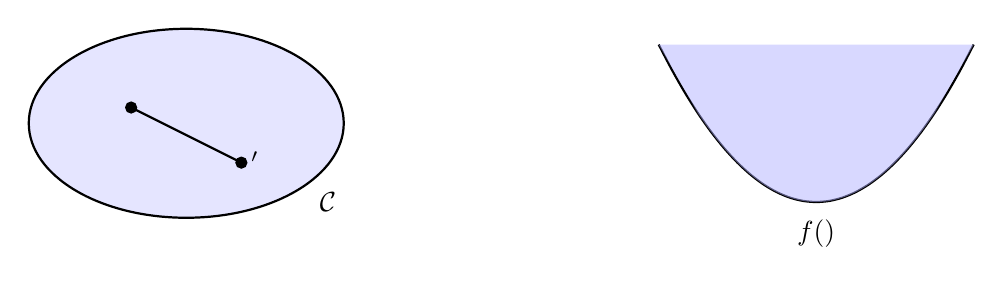
\begin{tikzpicture}
				% Left part: Convex set (Ellipse)
				\fill[blue!20, opacity=0.5] (-3,0) ellipse (2 and 1.2); % Shaded ellipse
				\draw[thick] (-3,0) ellipse (2 and 1.2);
			 % Points inside the ellipse
				\filldraw[black] (-3.7,0.2) circle (2pt) node[left] {$\vw$};
				\filldraw[black] (-2.3,-0.5) circle (2pt) node[right] {$\vw'$};
				% Line segment connecting the two points
				\draw[thick] (-3.7,0.2) -- (-2.3,-0.5);
				% Label for the convex set
				\node at (-1.2,-1.0) {$\mathcal{C}$};
				% Right part: Convex function and epigraph
				\begin{scope}[shift={(5,-1)}]
					% Define the convex function
					\draw[thick, domain=-2:2, smooth, variable=\x] 
					plot ({\x}, {0.5*\x*\x});
					% Shaded epigraph (area above the function)
					\fill[blue!30, opacity=0.5] 
					plot[domain=-1.5:1.5, smooth] ({\x}, {0.5*\x*\x}) -- 
					(2, {0.5*2*2}) -- 
					(-2, {0.5*2*2}) -- 
					cycle;
					%\fill[blue!30, opacity=0.5] (-1.5,1.2) -- (-1.5,2.5) -- (1.5,2.5) -- (1.5,1.2) -- plot[domain=-1.5:1.5, smooth] ({\x}, {0.5*\x*\x}) -- cycle;
					% Labels
					\node at (0,-0.4) {$f(\weights)$};
				\end{scope}
			\end{tikzpicture}
			\vspace*{-8mm}
			\end{center}
			\caption{Left: A convex set $\cluster \subseteq \mathbb{R}^{\dimlocalmodel}$. 
				Right: A convex function $f: \mathbb{R}^{\dimlocalmodel} \rightarrow \mathbb{R}$.\label{fig_convex_set_function}}
		\end{figure}},first={convex},text={convex}}


\newglossaryentry{smooth}{name={smooth},
	description={A\index{smooth} real-valued function $f: \mathbb{R}^{\dimlocalmodel} \rightarrow \mathbb{R}$ 
		is smooth if it is \gls{differentiable} and its \gls{gradient} $\nabla f(\weights)$ is continuous at all $\weights \in \mathbb{R}^{\dimlocalmodel}$  \cite{nesterov04,CvxBubeck2015}. A smooth function $f$ is referred to as $\beta$-smooth if the \gls{gradient} 
		$\nabla f(\weights)$ is Lipschitz continuous with Lipschitz constant $\beta$, i.e., 
		$$\| \nabla f(\weights) - \nabla f(\weights') \| \leq \beta \| \weights - \weights' \| \mbox{, for any } \weights,\weights' \in \mathbb{R}^{\dimlocalmodel}.$$ 
		The constant $\beta$ quantifies the amount of smoothness of the function $f$: the smaller the $\beta$, 
		the smoother $f$ is. Optimization problems with a smooth \gls{objfunc} can be solved effectively by \gls{gdmethods}. 
	    Indeed, \gls{gdmethods} approximate the \gls{objfunc} locally around a current choice $\weights$ 
	    using its \gls{gradient}. This approximation works well if the \gls{gradient} does 
	    not change too rapidly. We can make this informal claim precise by studying the effect of a single 
	    \gls{gradstep} with \gls{stepsize} $\lrate=1/\beta$ (see Figure \ref{fig_gd_smooth_dict}). 
	    \begin{figure}[H] 
	    	\begin{center} 
	    	\begin{tikzpicture}[scale=0.8, x=0.7cm,y=0.05cm]
	    		% Parameter to shift the quadratic curve horizontally
	    		\def\hshift{0.5} % Change this value to shift the curve horizontally
	    		% Define the function (only the increasing part of x^2 for x >= 0)
	    		\draw[thick, domain=\hshift:8+\hshift, smooth, variable=\x] plot ({\x}, {\x^2}); %node[right] {$f(x) = x^2$};
	    		% Define points for the tangents
	    		\coordinate (w) at (\hshift,{\hshift*\hshift}); % Point w on the curve (left end of the plot)
	    		\coordinate (wkplus1) at (4+\hshift,{(4+\hshift)^2}); % Point w^{k+1} on the curve (x=1 + hshift, y=1)
	    		\coordinate (wk) at (8+\hshift,{(8+\hshift)^2}); % Point w^k on the curve (right end of the plot)
	    		% Calculate the slopes for the tangents
  				\draw[line width=1pt, transform canvas={yshift=-2pt}] (wk) -- +(-1, -{2*(8 + \hshift)} ) -- +(1, {2*(8 + \hshift)}); % Tangent at w^k with positive slope
 				\draw[line width=1pt, transform canvas={yshift=-2pt}] (w) -- +(-1, -{2*\hshift} ) -- +(1, {2*\hshift} )  node[below] {$\nabla f(\weights)$};% Tangent at w with slope 0 (since derivative at hshift = 0)
%	    		% Draw filled circles at points w^k, w, and w^{k+1}
	    		\filldraw (wk) circle (2pt) node[above left] {$\weights^{(\iteridx)}$} node[below right] {$\nabla f(\weights^{(\iteridx)})$} ;
	    		\filldraw (w) circle (2pt) node[above right] {$\weights$} ;
	    		\filldraw (wkplus1) circle (2pt) node[below right] {$\weights^{(\iteridx+1)}\!=\!\weights^{(\iteridx)}\!-\!(1/\beta)\nabla f(\weights^{(\iteridx)})$};
	    		    % Draw horizontal rulers to mark the function values at wk and wk_plus1
	    		\draw[dashed] (wk) -- ($(8,0) + (wk)$) ; %node[left] {$f(\weights^{(\iteridx)})$};
	    		\draw[dashed] (wkplus1) -- ($(12,0) + (wkplus1)$) ; %node[left] {$f(\weights^{(\iteridx+1)})$};
	    		 \draw[<->, thick] ($(4,0) + (wk)$) -- ($(8,0) + (wkplus1)$) 
	    		node[midway, right] {$ f\big(\weights^{(\iteridx)}\big)\!-\!f\big(\weights^{(\iteridx+1)}\big)\!\geq\!\frac{1}{2\beta}\normgeneric{\nabla f(\weights^{(\iteridx)})}{2}^{2}$};
%	    		% Label the curve
%	    		\node at (2, 4) {};
	    	\end{tikzpicture}
	    	\end{center}
	    	\caption{Consider an \gls{objfunc} $f(\weights)$ that is $\beta$-smooth. 
	    		Taking a \gls{gradstep}, with \gls{stepsize} $\lrate = 1/\beta$, decreases the 
	    		objective by at least $\frac{1}{2\beta}\normgeneric{\nabla f(\weights^{(\iteridx)})}{2}^{2}$ \cite{nesterov04,CvxAlgBertsekas,CvxBubeck2015}. 
	    		Note that the \gls{stepsize} $\lrate = 1/\beta$ becomes larger for smaller $\beta$. Thus, 
	    		for smoother \gls{objfunc}s (i.e., those with smaller $\beta$), 
				we can take larger steps. \label{fig_gd_smooth_dict}}
	    	\end{figure}
	    },first={smooth},text={smooth}}

\newglossaryentry{paramspace}{name={parameter space},
		description={The\index{parameter space} parameter space $\paramspace$ of 
		an \gls{ml} \gls{model} $\hypospace$ is the set of all feasible choices for the 
		\gls{modelparams} (see Figure \ref{fig_param_space_dict}). Many important \gls{ml} methods 
		use a \gls{model} that is parametrized by vectors of the \gls{euclidspace} $\mathbb{R}^{\dimlocalmodel}$. 
		Two widely used examples of parametrized \gls{model}s are \gls{linmodel}s 
		and \gls{deepnet}s. The parameter space is then often a subset $\paramspace \subseteq \mathbb{R}^{\dimlocalmodel}$, 
		e.g., all vectors $\weights \in \mathbb{R}^{\dimlocalmodel}$ with a \gls{norm} smaller than one.
		\begin{figure}[H]
			\begin{center}
			\begin{tikzpicture}
				% Left part: Ellipse representing parameter space (with two dots)
				\node[ellipse, minimum width=3cm, minimum height=2cm, draw, thick] (paramspace) {};
				\node[below=0.1cm of paramspace] {parameter space $\paramspace$};
				% Two dots inside the left ellipse
				\node[black, circle, inner sep=2pt, fill] (theta1) at ($(paramspace.north west) + (1, -1)$) {};
				\node[left=0.01cm of theta1] {$\weights$};
				\node[black, circle, inner sep=2pt, fill] (theta2) at ($(paramspace.south east) + (-1.5, 1)$) {};
				\node[left=0.01cm of theta2] {$\weights'$};
				% Right part: Ellipse containing two smaller plots
				\node[ellipse, minimum width=7cm, minimum height=3cm, draw, thick, right=4cm of paramspace] (plotcloud) {};
				\node[above=0.2cm of plotcloud] {\gls{model} $\hypospace$};
				% Axis for first smaller plot
				\node (plot1start) at ($(plotcloud.south west) + (0.2, 0.2)$) {};
				%\draw[thick, ->] (plot1start) -- ++(2, 0) node[anchor=north] {$\featurevec$};
				%\draw[thick, ->] (plot1start) -- ++(0, 1.5) node[anchor=east] {$\truelabel$};
				% Simple plot line in first smaller plot
				\draw[thick, red] (plot1start) .. controls ++(0.8, 1) and ++(-0.8, -0.8) .. ($(plotcloud.south west) + (2.8, 0.8)$) node[anchor=west] {$\hypothesis^{(\weights)}$};
				% Axis for second smaller plot
				\node (plot2start) at ($(plotcloud.south west) + (1.0, 1.2)$) {};
			%	\draw[thick, ->] (plot2start) -- ++(2, 0) node[anchor=north] {$\featurevec$};
			%	\draw[thick, ->] (plot2start) -- ++(0, 1.5) node[anchor=east] {$\truelabel$};
				% Simple plot line in second smaller plot
				\draw[thick, blue] (plot2start) .. controls ++(0.8, 0.5) and ++(-0.8, -0.8) .. ($(plotcloud.south west) + (2.8, 2.1)$) node[anchor=west] {$\hypothesis^{(\weights')}$};
				% Connect the two dots in the parameter space to the two plots
				\draw[thick, ->, bend right=20] (theta1) to ($(plot1start) + (0,0)$);
				\draw[thick, ->, bend left=20] (theta2) to (plot2start);
			\end{tikzpicture}
			\end{center} 
			\caption{The parameter space $\paramspace$ of an \gls{ml} \gls{model} $\hypospace$ consists of all 
			feasible choices for the \gls{modelparams}. Each choice $\weights$ for the \gls{modelparams} 
			selects a \gls{hypothesis} map $\hypothesis^{(\weights)} \in \hypospace$.
				 \label{fig_param_space_dict}} 
\end{figure}},
			first={parameter space},text={parameter space}}

\newglossaryentry{datanorm}{name={data normalization},
	description={\Gls{data} normalization\index{data normalization} refers to transformations 
		applied to the \gls{featurevec}s of \gls{datapoint}s to improve the \gls{ml} method's 
		\gls{statasp} or \gls{compasp}. For example, in \gls{linreg} with \gls{gdmethods} using 
		a fixed \gls{learnrate}, convergence depends on controlling the \gls{norm} of \gls{featurevec}s 
		in the \gls{trainset}. A common approach is to normalize \gls{featurevec}s such that their 
		\gls{norm} does not exceed one \cite[Ch.\ 5]{MLBasics}.},
	first={data normalization},text={data normalization}}

\newglossaryentry{dataaug}{name={data augmentation},
	description={\Gls{data} augmentation\index{data augmentation} methods add synthetic \gls{datapoint}s 
		to an existing set of \gls{datapoint}s. These synthetic \gls{datapoint}s are obtained by 
		perturbations (e.g., adding noise to physical measurements) or transformations 
		(e.g., rotations of images) of the original \gls{datapoint}s. These perturbations and 
		transformations are such that the resulting synthetic \gls{datapoint}s should 
		still have the same \gls{label}. As a case in point, a rotated cat image is still 
		a cat image even if their \gls{featurevec}s (obtained by stacking pixel color intensities) 
		are very different (see Figure \ref{fig_symmetry_dataaug_dict}). \Gls{data} augmentation can be an 
		efficient form of \gls{regularization}.
		\begin{figure}[H]
		\begin{center}
			\begin{tikzpicture}
				% Define shift macros locally
				\newcommand{\xshift}{0.5}
				\newcommand{\yshift}{2}
				% Define the shifted curves
				% Define the shifted curves
  				\draw[very thick, blue] plot[smooth, tension=1] coordinates {(0,0) (2,1) (4,0) (6,-1) (8,0)};
  				\node[blue, right] at (0,0) {\textbf{cat}};
  				\draw[very thick, red, dashed] plot[smooth, tension=1] coordinates {(0 + \xshift,0 + \yshift) (2 + \xshift,1 + \yshift) (4 + \xshift,0 + \yshift) (6 + \xshift,-1 + \yshift) (8 + \xshift,0 + \yshift)};
  				\node[red, right] at (8 + \xshift,0 + \yshift) {\textbf{no cat}};
				\fill[blue] (2,1) circle (2pt) node[above] {$\featurevec^{(1)}$};
				\fill[blue] (6,-1) circle (2pt) node[above] {$\featurevec^{(2)}$};
				  % Draw a bent arrow connecting the two points with custom in and out angles
				  \draw[->, thin, >=latex, line width=0.5pt] (2,1) to[out=240, in=240] node[midway, below] {$\mathcal{T}^{(\eta)}$} (6,-1);
			  \end{tikzpicture}
			  \vspace*{-11mm}
		\end{center}
		\caption{\Gls{data} augmentation exploits intrinsic symmetries of \gls{datapoint}s in 
		       some \gls{featurespace} $\featurespace$. We can represent a symmetry by 
		     an operator $\mathcal{T}^{(\eta)}: \featurespace \rightarrow \featurespace$,
		     parametrized by some number $\eta \in \mathbb{R}$. For example, $\mathcal{T}^{(\eta)}$ 
		    might represent the effect of rotating a cat image by $\eta$ degrees. A \gls{datapoint} 
		    with \gls{featurevec} $\featurevec^{(2)} = \mathcal{T}^{(\eta)} \big(\featurevec^{(1)} \big)$ must 
		    have the same \gls{label} $\truelabel^{(2)}=\truelabel^{(1)}$ as a \gls{datapoint} 
		     with \gls{featurevec} $\featurevec^{(1)}$.\label{fig_symmetry_dataaug_dict}}
		 \end{figure} },first={data augmentation},text={data augmentation}}
	
	
\newglossaryentry{localdataset}{name={local dataset},description={The\index{local dataset} concept of a local \gls{dataset} is 
		in between the concept of a \gls{datapoint} and a \gls{dataset}. A local \gls{dataset} consists of several 
		individual \gls{datapoint}s, which are characterized by \gls{feature}s and \gls{label}s. 
		In contrast to a single \gls{dataset} used in basic \gls{ml} methods, a local \gls{dataset} is also 
		related to other local \gls{dataset}s via different notions of similarity. These similarities 
		might arise from \gls{probmodel}s or communication infrastructure and 
		are encoded in the edges of an \gls{empgraph}.},first={local dataset},text={local dataset}}
	
\newglossaryentry{localmodel}{name={local model},description={Consider\index{local model} a collection 
		of \gls{localdataset}s that are assigned to the nodes of an \gls{empgraph}. A local \gls{model} $\localmodel{\nodeidx}$ 
		is a \gls{hypospace} assigned to a node $\nodeidx \in \nodes$. Different nodes might be assigned 
		different \gls{hypospace}s, i.e., in general $\localmodel{\nodeidx} \neq \localmodel{\nodeidx'}$ for different 
		nodes $\nodeidx, \nodeidx' \in \nodes$.  },first={local model},text={local model}}
	
\newglossaryentry{mutualinformation}
{name={mutual information (MI)},
 description={The\index{mutual information (MI)} MI $\mutualinformation{\featurevec}{\truelabel}$ 
 	between two \gls{rv}s $\featurevec$, $\truelabel$ defined on the same \gls{probspace} 
 	is given by \cite{coverthomas} $$\mutualinformation{\featurevec}{\truelabel} \defeq 
	\expect \left\{ \log \frac{p (\featurevec,\truelabel)}{p(\featurevec)p(\truelabel)} \right\}.$$ 
	It is a measure of how well we can estimate $\truelabel$ based 
	solely on $\featurevec$. A large value of $\mutualinformation{\featurevec}{\truelabel}$ indicates that 
	$\truelabel$ can be well predicted solely from $\featurevec$. This \gls{prediction} could be obtained by a 
		\gls{hypothesis} learned by an \gls{erm}-based \gls{ml} method. 
	 }, first={MI}, text={MI} 
}

\newglossaryentry{zerogradientcondition}{name={zero-gradient condition},
	description={Consider\index{zero-gradient condition} the unconstrained 
		optimization problem $\min_{\weights \in \mathbb{R}^{\dimlocalmodel}} f(\weights)$  with 
			a \gls{smooth} and \gls{convex} \gls{objfunc} $f(\weights)$. A necessary and 
			sufficient condition for a vector $\widehat{\weights} \in \mathbb{R}^{\dimlocalmodel}$ 
			to solve this problem is that the \gls{gradient} $\nabla f \big( \widehat{\weights} \big)$ 
			is the zero vector, 
			$$ \nabla f \big( \widehat{\weights} \big) = \mathbf{0} \Leftrightarrow  f \big( \widehat{\weights} \big) = \min_{\weights \in \mathbb{R}^{\dimlocalmodel}} f(\weights) .$$ }, 
			first={zero-gradient condition},text={zero-gradient condition}}


\newglossaryentry{edgeweight}{name={edge weight},
	description={Each\index{edge weight} edge $\edge{\nodeidx}{\nodeidx'}$ of an \gls{empgraph} is 
		assigned a non-negative edge weight $\edgeweight_{\nodeidx,\nodeidx'}\geq0$. 
		A zero edge weight $\edgeweight_{\nodeidx,\nodeidx'}=0$ indicates the absence 
		of an edge between nodes $\nodeidx, \nodeidx' \in \nodes$.}, 
	first={edge weight},text={edge weight}}


\newglossaryentry{dataminprinc}{name={data minimization principle},
	description={European\index{data minimization principle} \gls{data} protection regulation 
		includes a \gls{data} minimization principle. This principle requires a \gls{data} controller to 
		limit the collection of personal information to what is directly relevant and necessary 
		to accomplish a specified purpose. The \gls{data} should be retained only for as long as 
		necessary to fulfill that purpose \cite[Article 5(1)(c)]{GDPR2016}, \cite{EURegulation2018}.}, 
	first={data minimization principle},text={data minimization principle}}


